\documentclass[usenatbib]{mnras}
\usepackage[utf8]{inputenc}
\usepackage[T1]{fontenc}
\usepackage{graphicx}
\usepackage{grffile}
\usepackage{longtable}
\usepackage{wrapfig}
\usepackage{rotating}
\usepackage[normalem]{ulem}
\usepackage{amsmath}
\usepackage{textcomp}
\usepackage{amssymb}
\usepackage{capt-of}
\usepackage{hyperref}
\usepackage{natbib}
\usepackage{varioref}
\usepackage{bm}
\usepackage{pgfplots}
\usepackage[nameinlink, capitalize, noabbrev]{cleveref}

\usepgfplotslibrary{groupplots,dateplot}
\usetikzlibrary{patterns,shapes.arrows,external}
\tikzexternalize
\pgfplotsset{compat=newest}
\usepackage{dsfont}
\usepackage{xcolor}
\usepackage{listings}

\DeclareMathOperator{\TopHat}{TH}
\DeclareMathOperator{\CDF}{CDF}

\author[A. Petrosyan and W. J. Handley]{
  Aleksandr Petrosyan,$^{1}$
  William James Handley$^{2}$
  \\
  $^{1}$ University of Cambridge, Queens' College, Silver st., Cambridge, CB3 9ET, UK\\
  $^{2}$ University of Cambridge, Kavli Institute of Astronomy, Madingley Road, Cambridge, CB3 0HA, UK 
}
\date{\today}
\title[Stochastic posterior repartitioning]{Bayesian Machine learning in context of cosmological parameter estimation}
\hypersetup{
 pdfauthor={Aleksandr Petrosyan, William James Handley},
 pdftitle={Bayesian Machine learning in context of cosmological parameter estimation},
 pdfkeywords={},
 pdfsubject={},
 pdfcreator={Emacs 26.3 (Org mode 9.1.9)}, 
 pdflang={English}}
\crefname{Option}{Option}{Options}
\crefname{Property}{Property}{Properties}

\begin{document}

\maketitle
\begin{abstract}
Bayesian inference is one of the most robust scientific hypothesis testing frameworks. It is utilised in many areas of physics that require detailed analysis of the underlying hypothesis. Cosmology, one such field is faced with challenges due to the complexity of the underlying theory, making inference computationally expensive even with the state of the art Bayesian inference software:  nested sampling packages like \texttt{PolyChord}. We here present a methodology that allows one to simultaneously improve the robustness and accelerate nested sampling based Bayesian inference. In this paper we introduce a formal mathematical framework that explicates previous work in the field, as well as allows further developments to be made. We subsequently introduce three other methodologies for conducting repartitioning: argument scaling, boundary re-sizing and superpositional mixing. We demonstrate that these techniques are able to produce more accurate and more precise results, while also \emph{significantly} improving run-time characteristics of the nested sampling package they're used with. Finally, as a demonstration of its most lucrative application, we demonstrate that it is able to reduce the execution time of a \texttt{Cobaya}/\texttt{CLASS} based cosmological parameter inference by a factor of TODO. 

\end{abstract}

\begin{keywords}
Bayesian inference -- automated posterior repartitioning -- nested sampling -- cosmology: miscellaneous -- methods: statistical -- methods: data analysis
\end{keywords}

\section{Introduction}\label{sec:org14413d7}

The standard model of the universe and its evolution in modern
cosmology is the \(\Lambda\)CDM model \citep{Condon2018}, so named
after the main components of the universe: the \emph{cosmological constant} \(\Lambda\)
and \emph{cold dark matter}. It has six major independent parameters:
physical baryon density \(\Omega_{b}h^{2}\); physical dark matter
density \(\Omega_{c}h^{2}\); the age of the universe \(t_{0}\); scalar
spectral index \(n_{s}\); curvature fluctuation amplitude
\(\Delta_{R}^{2}\); and re-ionization optical depth \(\tau\). It is the
task of the present study to \emph{develop better tools} for estimating
the agreement of our observations from the Planck mission with
\(\Lambda\)CDM, simultaneously estimating the parameters. In this
section we shall describe the main approaches, as well as the
refinements to these approaches that we have developed.

The above makes Bayesian inference a convenient methodology for
estimating cosmological parameters. Hence a large number of algorithms
was developed to accelerate the computation: Metropolis-Hastings
\citep{Metropolis} in conjunction with the Gibbs sampler
\citep{Metropolis-Hastings-Gibbs}; Hybrid (Hamiltonian) Monte Carlo
\citep{1701.02434,Duane_1987}, and --- nested Sampling
\citep{Skilling2006}, which we shall focus on.

Nested sampling~\cite{Skilling2006} is a family of algorithms, each
with their own unique implementation details:
\begin{enumerate}
\item \texttt{MultiNest} \citep{Feroz2009MultiNestAE},
\item \texttt{nestle} \citep{nestle}
\item \texttt{dyNesty} \citep{Speagle_2020},
\item \texttt{PolyChord} \citep{polychord}.
\end{enumerate}
to name a few major implementations.

We have \emph{discovered} a method accelerates \emph{all}  nested sampling
implementations, each to a different extent. The following paper, was
primarily tested with \texttt{PolyChord}, however other samplers
should (and do) see similar performance gains.

Our optimisation is based on the observation due
to~\cite{chen-ferroz-hobson}, that the nested sampling algorithm,
unlike other Markov-chain Monte Carlo Bayesian inference methods, is
sensitive to how the posterior is partitioned into the two conditional
probabilities: \emph{likelihood} and \emph{prior}, with respect to the
posterior distribution. They used this to develop a technique ---
\emph{automatic power posterior repartitioning} (PPR), that they used
to improve the stability of convergence for prior distributions that
may have been at variance with the true posterior.

We have found a \emph{generalisation} of this technique, and showed
that it can be used to \emph{significantly} accelerate the convergence.

We've developed the mathematical framework that encapsulates the idea
and explores the extents of its utility. In particular, we have found
a way to describe \emph{how} one may achieve better stability and
better performance. We also present a numerical application of this
framework in terms of the following techniques that we have developed:
mixture repartitioning (superpositional and additive) and re-sizeable
bounds uniform repartitioning, as well as demonstrated that PPR can
be used to heuristically accelerate nested sampling.

\section{Theoretical background}\label{sec:orge6061a4}

\subsection{Bayesian inference}\label{sec:org6b7d2fe}

This topic has been discussed at length in literature
\citep{jeffreys2010scientific}, so we shall restrict ourselves to the
minimum required to understand what follows.

Let \({\cal M}\) be a model of some process, parameterised with
\[\bm{\theta} = (\theta_{1}, \theta_{2}, \ldots ,
  \theta_{n}).\] Meaning that it defines a probability distribution of
physical observables ${\cal O}_\text{predicted}$, contingent on model
parameters \(\bm{\theta}\). Actual experimental values of
${\cal O}_\text{actual}$ encapsulated in \(\mathfrak{D}\). From these
we build conditional probabilities. In the language of
\cref{table-defs}, \citeauthor{1763}'s theorem is
\begin{equation}\label{eq:bayes} 
 {\cal L} \times \pi (\bm{\theta}) = {\cal Z}\times {\cal P} (\bm{\theta}).
\end{equation}
With \emph{evidence} \({\cal Z}\) 
\begin{equation}\label{eq:def-z}
 {\cal Z} \triangleq \int_{\Psi} {\cal L}(\theta) \pi(\theta) d\theta, 
\end{equation}
where \(\Psi\) is the \emph{prior space} --- the domain of 
\(\pi(\bm{\theta})\).\footnote{\Cite{jeffreys2010scientific} believes \({\cal Z}\) to be no more than a normalisation factor, but by definition (see Table~\vref{table-defs}), it quantifies the consistency of the hypothesis with  observation. Essentially,  higher \({\cal Z}\), implies higher accuracy of our model.}

\begin{table}
  \caption{Definitions of main quantities in Bayesian analysis. PDF means \textbf{p}robability \textbf{d}ensity \textbf{f}unction, PVE --- \textbf{p}arameter \textbf{v}olume \textbf{e}lement, i.e. \(d \bm{\theta}\). Units given for reference, but also to emphasise the use of density functions, vs.\ cumulative distributions.\label{table-defs}}
\centering
\begin{tabular}{llrr}
\textbf{\textbf{Term}} & \textbf{\textbf{Symbol}} & \textbf{\textbf{Definition}} & \textbf{\textbf{Units}}\\
\hline
Prior (PDF) & \(\pi(\theta)\) & \(P ( \theta  \vert {\cal D})\) & PVE\(^{-1}\)\\
Likelihood (PDF) & \({\cal L}(\theta)\) & \(P ( {\cal D} \vert \bm{\theta} \cup M)\) & PVE\(^{-1}\)\\
Posterior (PDF) & \({\cal P}(\theta)\) & \(P ( \theta \vert {\cal D} \cup M)\) & PVE\(^{-1}\)\\
Evidence & \({\cal Z}\) & \(P ( {\cal D} \vert {\cal M})\) & arbitrary units\\
\end{tabular}
\end{table}

The two independent functions, \({\cal L}(\bm{\theta})\) and
\(\pi(\bm{\theta})\) are inputs to Bayesian inference machine
(sampler). Their convenient depiction depends on the particular
sampling algorithm, however, for most nested samplers
(e.g. \texttt{PolyChord}, \texttt{MultiNest}) we delineate them indirectly with
log-likelihood:
\begin{equation*}
  L(\bm{\theta}) = \ln \cal L (\bm{\theta})
\end{equation*}
and \emph{prior quantile} \(C\{\pi\}(\bm{\theta})\), which is the
\emph{inverse cumulative distribution function} (iCDF) of random
variable \(\bm{\theta}\) with the probability density function
\(\pi(\bm{\theta})\). Specifically,
\begin{equation*}
 C\{\pi\} : \text{unit hyper-cube} \rightarrow \Psi;
\end{equation*}
a mapping from a unit hypercube (where the distribution of the images
of parameters \(\bm{\theta}\) is uniform), onto the prior space
\(\Psi\).

Note, that there is a redundancy in our specification of \({\cal
   L}(\bm{\theta})\) and \(\pi(\bm{\theta})\).  Consider a
different pair of functions \(\tilde{{\cal L}}(\bm{\theta})\) and
\(\tilde{\pi}(\bm{\theta})\), such that
\begin{equation}\label{eq:redundancy}
  \tilde{\cal L}(\bm{\theta}) \tilde{\pi}(\bm{\theta}) = \cal L (\bm{\theta}) \pi (\bm{\theta}), 
\end{equation}
for all \(\bm{\theta} \in \Psi\). In this representation, the
value of \({\cal Z}\) is unchanged, hence by \cref{eq:bayes},
\({\cal P}(\bm{\theta})\) is also. Thus, \emph{most} Bayesian samplers
are indifferent to concrete definitions of \(\cal L\) and \(\pi\),
as long as their product --- the posterior, corresponds to the same
model. However, nested sampling \emph{is} sensitive to the
\emph{partitioning} of the \({\cal P} (\bm{\theta})\) into \({\cal L}(\bm{\theta})\)
and \(\pi(\bm{\theta})\), which is the centerpiece of the techniques
discussed earlier. While as we mentioned it must obtain the same
evidence and the same posterior, remarkably it may obtain those
much more quickly for some choices of \(\tilde{\pi}\). In the next
section we shall elaborate on that point.

\subsection{Nested Sampling}\label{sec:org36366f8}

Bayes' theorem reduces the problem of parameter estimation to
integration. Thus the naïve approach: uniformly rasterise \(\Psi\) and
\({\cal Z}\) via Riemann sums, is valid. However, for hypotheses with
\(O(30)\) parameters, said rasterisation is intractable
\citep{Caflisch_1998} and integration is done using Monte Carlo
techniques. Nested sampling is one such technique that has
considerable performance advantages in high-dimensional many-parameter
models.

Consider without loss of generality, a prior space \(\Psi\) that is a
unit hypercube, where \[\pi(\bm{\theta}) = \text{Const.}\] Draw
\(n_\text{live}\) random \emph{live points} from the unit
hypercube. If \({\cal L}\) is a well-behaved function, the probability
that two points have the same likelihood is vanishing, so each of them
lies on a \textbf{distinct} iso-likelihood
hyper-surface\footnote{analogy: height on a contour map. }. Each
hyper-surface encloses the fraction
\begin{equation}
\cfrac{1}{n_\text{live}}
\end{equation}
of the total volume of the hypercube on average. More specifically,
each shell's enclosed volume shall have some random deviation \(\Delta\), from
\(\cfrac{1}{n_\text{live}}\), with an associated cumulative
distribution \(P(\Delta)\).

Subsequently, we pick another point at random, requiring that the
likelihood of the new point be higher than the lowest likelihood of
the initial \emph{live point} ensemble. In \citeauthor{Skilling2006}'s
notation, the point with the lowest likelihood becomes \emph{dead} and
the new point becomes is \emph{live}. This is a single iteration of
nested sampling.

Our argument of approximately equal volumes holds for the new
ensemble, so the volume encased in the outer-most shell iteratively
reduces by the same fraction, allows us to approximate said volumes:
\begin{equation}\label{eq:recurrence-relation}
  \begin{array}{rcl}
  X_{0} &=  &1, \\
  X_{1} &= &X_{0} \left(1- \cfrac{1}{n_\text{live}}\right),\\
  & \vdots &, \\
  X_{i} &= &X_{i-1}\left(1- \cfrac{1}{n_\text{live}}\right),\\
  & \vdots, &
\end{array}
\end{equation}
Thus we iteratively pick live points in regions $\{\bm{\theta}\}$ of
high \({\cal L}\), and also estimating the evidence, and stop when the
prior volume encased in the outer shell is lower than a predetermined
fraction e.g. \(0.01\) of the original hypercube volume.

The recurrence relation~\eqref{eq:recurrence-relation} is not exact,
however, \(P(\Delta)\) is a known distribution, dependent on the
\(\dim \Psi\) and \({\cal L}\). Thus, for each \(\epsilon>0\), we
exists
\[\delta(\epsilon) >0,\] such that \[P(\Delta > \delta)<\epsilon.\]
Hence, by choosing \(\epsilon\) based on \(n_\text{live}\), one
obtains an estimate of the error \(\delta\). Propagating these errors
allows us to evaluate the prior volume, ergo: ${\cal Z}$ up to an
estimable error.

This is generalised to non-hypercube $\Psi$ and non-uniform $\pi$ via
the prior quantile. 

The time complextity of nested sampling $T$ satisfies the following
relations.
\begin{subequations}\label{eq:complexity}
  \begin{align}
    T \propto & n_\text{live}\\
    T \propto & \langle {\cal T}\{{\cal L}(\bm{\theta})\} \rangle
  \end{align}
\end{subequations}
where ${\cal T}$ represents time complexity of the
function. Corollary: \emph{rejection sampling} --- drawing a point at random,
and re-drawing at random based on the criteria mentioned, is less
efficient than \emph{slice sampling} \citep{Neal_2003}.

Generally, if the prior is informative, one can design an
implementation of nested sampling which incorporates that extra
information, to accelerate nested sampling --- an ideal sampler. It
would converge optimally when the prior and the posterior coincide:
\begin{equation}
\begin{array}{rl} 
{\cal P}(\bm{\theta}) = \pi(\bm{\theta}), & \forall \bm{\theta}. 
\end{array}
\end{equation}
Many algorithms, however, may have minimum run-time for non-coinciding
informative priors.

\subsection{Unrepresentative priors\label{discussion-bias}}
The choice of prior is relatively arbitrary, yet we have
demonstrated that one can choose them differently accelerating
inference.

So why not just adjust our prior based on intuition?  To illustrate,
consider that one has gathered data from free fall experiments. On
earth, one knows the posterior for \(g\) to be a normal distribution
peaked at \[\langle g \rangle=9.81,\] with standard
deviation \[\sigma_{g} = 0.01\] due to regional variations, which we
shall compactly refer to as
\begin{equation*}
  \pi(\bm{\theta}) = G(\bm{\theta};\bm{\mu}_{g}=9.81, \bm{\sigma}_{g}=0.01, \ldots ).
\end{equation*}
We use this to obtain a posterior distribution.

So if one chooses a prior without changing the likelihood, the
posterior would be different. If the prior changed due to new
information, this is desired. If the prior was chosen ad-hoc, this
limits the utility of the posterior and evidence.


This is the problem of \emph{unrepresentative priors} and
\citeauthor*{chen-ferroz-hobson} have developed power-posterior
repartitioning specifically as a mitigation of this issue. 

\subsection{Power posterior repartitioning}\label{sec:org68fff63}

\citeauthor{chen-ferroz-hobson} have proposed introducing an
extra parameter \(\beta\) that re-scales the prior:
\begin{equation*}
  \tilde{\pi}(\bm{\bm{\theta}};\beta) = \cfrac{\pi(\bm{\theta})^{\beta}}{Z(\beta)\{\pi\}},
\end{equation*}
where \(Z(\beta)\{\pi\}\) is a normalisation factor, i.e. 
\begin{equation*}
  Z(\beta)\{\pi\} = \int_{\bm{\theta} \in \Psi} \pi(\bm{\bm{\theta}})^{\beta}d\bm{\bm{\theta}}.
\end{equation*}
In their prescription, the likelihood changes to
\begin{equation*}
  \tilde{\cal L}(\bm{\theta}) = {\cal L}(\bm{\theta}) Z(\beta)\{\pi\} \cdot \pi^{1-\beta}(\bm{\theta}).
\end{equation*}
The domains of all functions need to be the same. Let
\(D(f)\) denote the domain of the function \(f\), i.e.~where the
function is both defined and \textbf{non-zero}. Hence
\begin{equation*}
  D(\pi) = D({\cal L}) = \Psi = D({\cal P}),
\end{equation*} 
meaning the posterior is within the domain of the prior and
likelihood, which will be important later.\label{domain-discussion}

There is no general prescription for determining the prior of
\(\beta\). The tightest constraints on \(\beta\) produce the best
convergence speed, however broad constraints may be valuable.  If
\(\pi(\bm{\theta})\) is Gaussian, a uniform 
\[\beta\in[0,1]\] prior is a convenient starting point.
If the original prior \(\pi\) was representative, one could introduce
a non-linear map that favours \(\beta\approx 1\) making
\(\tilde{\pi}\) more representative. If the original prior may have
been too broad (overestimated errors) we could extend it
to \[\beta>1.\] Rarely, \[\beta<0,\] may also be useful.

This, for the cases that \citeauthor{chen-ferroz-hobson} have
originally considered, resolves the issue of non-representative
priors, because the evidence associated with the biased prior reduces
as \(\beta\rightarrow0\). This is meant to trade performance for
mitigating systematic errors, though faster than a uniform
prior.\footnote{in practice, the overhead associated with PPR is
  negligible, and even in the case of uni-variate examples, where the
  relative impact of adding an extra parameter is maximal, the
  overhead is insignificant~\cite[see][section ``numerical
  examples'']{chen-ferroz-hobson}.}

Notice that the \citeauthor{chen-ferroz-hobson}'s construction is
only useful if the prior we started with --- \(\pi\), was
peaked. Indeed, raising a uniform prior \(\pi\) to power \(\beta \in
   \mathbb{R}\) would not change it in any way.

\section{Theoretical discoveries}
\subsection{PPR for  accelerating convergence}

Our first discovery pertains to the inverted premise, where we guess a
prior to accelerate convergence.

We have a model \({\cal M}\), for which we have no prior knowledge,
hence the prior \(\pi\) is uniform.\footnote{the standard invariant
  objective prior in the general case was proven
  by~\cite{JeffreysPrior} to be the determinant of the fisher
  Matrix. A straightforward calculation thus yields that for a
  Gaussian distribution with a fixed standard deviation the Xprior is
  unity and unbounded, hence not normaliseable. Normally, however,
  it's assumed to be normalised and bounded.} Central limit theorem
suggests that the posterior may be a Gaussian:
\begin{equation}
 \pi (\bm{\theta}) \propto \exp \left[-\left(\cfrac{\bm{\theta} - \bm{\mu}}{2\bm{\sigma}}\right)^{2} \right],
 \label{eq:bias}
\end{equation}
where \(\bm{\mu}\) and \(\bm{\sigma}\) are unknown to us.\footnote{we
  have slightly abused the notation: the quotient of two vector
  quantities is undefined. Instead, in such fractions there is an
  implicit tensor index. Whenever a quantity with an implicit index is
  equated to a probability density, summation over the index is
  implied.} Based on our experience we may guess what these values may
be, without guarantee that either the shape or the location of the
posterior is given by \cref{eq:bias}.

We shall refer to this function as the \emph{intuition}, or the \emph{biased
prior}. This intuition is subjective, and therefore using it
directly, will negatively affect our posterior (\vref{discussion-bias}). Can one incorporate the useful
information if the guess is correct, without that biasing the
result? Using the guess as the initial prior \(\pi\) in PPR, seems to
produce what we need.

In detail: a point with random coordinates is drawn from an \(n+1\)
dimensional space with vectors:
\begin{equation}
  \tilde{\bm{\theta}} = (\theta_{1}, \theta_{2}, \ldots, \theta_{n}, \beta)
\end{equation}
where $\beta$ is treated by (nested sampling) the same as any other
component of \(\bm{\theta}\). This leads to live points with
$\tilde{\bm{\theta}}$ corresponding to higher ${\cal L}$, being
favoured. Consequently, the value of $\beta$ for which the prior is
similar to the posterior, is biased for.

This feedback ensures that if the true posterior is within the
region of radius \(\sigma / \beta\) of the guessed value of
\(\bm{\mu}\), then the new points are chosen preferentially from the
posterior region, including values of \(\beta\) that keep the
posterior region close to the prior peak. Specifically, if our
hypothesis were completely wrong, then the values of \(\beta
   \rightarrow 0\) would be favoured. The effective prior would then
tend to a uniform distribution. This is ensured by the
re-normalisation of \({\cal L}\).

\begin{figure}
 \input{./illustrations/ppr.tex}
\caption{\label{org44950de}
A demonstration of the function \(\tilde{\pi}(\bm{\theta}; \beta)\) for different values of \(\beta\). Note that we've started under the assumption that the distribution is a truncated Gaussian, i.e.~that it is zero outside the range \((-1, 1)\). This manifests as sharp changes in curvature at the boundaries. Note that \(\forall \beta\), \(\int_{-1}^{1}\tilde{\pi}(\bm{\theta}; \beta) = 1\).}
\end{figure}

Having demonstrated correctness, let's focus on performance. The
majority of the run-time of nested sampling with a uniform prior is
spent transplanting the live points onto the posterior
contour. With \(\beta>0\), the probability that points will be chosen
from high-likelihood regions is enhanced, so on-average the
execution time should decrease.

This is what we observe in practice: \cref{fig:benchmark}. 

\subsection{General automatic posterior repartitioning}

Let us recap the key components of posterior repartitioning. We
have a baseline uniform prior, with its likelihood \((\pi(\bm{\theta}),
   \cal L (\bm{\theta}))\), and a parameterised pair of biased prior and
likelihood \((\pi'(\bm{\theta}; \beta), \cal L' (\bm{\theta}; \beta))\), which
satisfy the following requirements.

\begin{enumerate}
\item For some \(\beta_{0}\), 
\begin{subequations}
\begin{align}
\tilde{\pi}(\bm{\theta}; \beta_{0}) &\equiv \pi(\bm{\theta}) \\
\tilde{\cal L}(\bm{\theta}, \beta_{0}) &\equiv {\cal L}(\bm{\theta})
\end{align}
\end{subequations}
known as the \textbf{specialisation property}.\label[Property]{spec-prop}
\item The product of the parameterised pair is constant for all values
of \(\beta\) and by~\cref{spec-prop}, 
\begin{equation*} 
\pi'(\bm{\theta}; \beta) \cal L'(\bm{\theta}; \beta) = \pi(\bm{\theta}) \cal L (\bm{\theta}),
\end{equation*}
which is the \textbf{normalisation property}.\label[Property]{norm-prop}
\item There's a guiding dynamical principle that favours the
representative prior \(\pi_{R}\), i.e. \(\beta\rightarrow\beta_{R}\)
that satisfies
\begin{equation*}
  \lim_{\beta\rightarrow\beta_{R}}\cfrac{\int \pi(\bm{\theta}, \beta) - \pi_{R}(\bm{\theta}) d\bm{\theta}}{\beta - \beta_{R}} = \min
\end{equation*}
which we call the \textbf{convergence property}.\label[Property]{vconv-prop}
\end{enumerate}

PPR satisfies all three properties as follows:~\vref{spec-prop} is
fulfilled with \[\pi'(\bm{\theta}; 0) =\pi(\bm{\theta}),\]~\cref{norm-prop} is
fulfilled by construction and~\cref{vconv-prop}, by noting that
\[\lim_{\beta \rightarrow 0} \pi'(\bm{\theta}; \beta) =
  \pi(\bm{\theta}).\]

Any pair of functions \(\pi'(\bm{\theta}; \beta)\),
\({\cal L}'(\bm{\theta}; \beta)\) that satisfy these requirements
constitute a repartitioning scheme. They are all guaranteed to yield
the same evidence and posterior, so our remaining task is to identify
schemes that produce better performance. In the following subsections
we shall consider several such possibilities.

\subsubsection{Additive mixtures.}\label{sec:org418133f}
Consider a weighted sum of a uniform distribution with
a Gaussian, e.g.~in one dimension
\begin{equation}\label{eq:additive-mix}
  \pi(\bm{\theta}) = \frac{ \left\lbrace \cfrac{1- \beta} {\bm{b} - \bm{a}} + \beta \exp \left[ -\left(\cfrac{\bm{\theta} - \bm{\mu}}{\bm{\sigma}} \right)^{2}\right]\right\rbrace \cdot \TopHat(\bm{\theta}; \bm{a}, \bm{b})}{Z}.
\end{equation}
where \[\TopHat(\bm{\theta};\bm{a},\bm{b}) = \prod_{i}
	\TopHat(\theta_{i}; a_{i}, b_{i})\] is the top-hat function. Integrate
to obtain the normalisation factor \(Z(\beta)\{\pi\}\), utilised
to re-scale \({\cal L}\). Recall, however, that we represent the
prior via the inverse of the cumulative distribution. The iCDF of
each component is usually known, however the iCDF of their sum, is
not guaranteed to be representable in closed form.

\begin{figure}
  % This file was created by tikzplotlib v0.9.1.
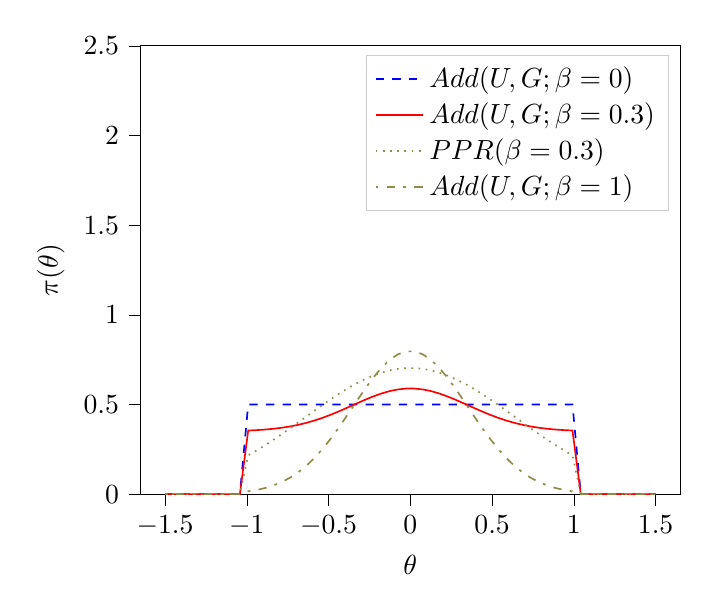
\begin{tikzpicture}

\begin{axis}[
legend cell align={left},
legend style={fill opacity=0.8, draw opacity=1, text opacity=1, draw=white!80!black},
tick align=outside,
tick pos=left,
x grid style={white!69.0196078431373!black},
xlabel={\(\displaystyle \theta\)},
xmin=-1.65, xmax=1.65,
xtick style={color=black},
y grid style={white!69.0196078431373!black},
ylabel={\(\displaystyle \pi(\theta)\)},
ymin=0, ymax=2.5,
ytick style={color=black}
]
\addplot [semithick, blue, dashed]
table {%
-1.5 0
-1.44915254237288 0
-1.39830508474576 0
-1.34745762711864 0
-1.29661016949153 0
-1.24576271186441 0
-1.19491525423729 0
-1.14406779661017 0
-1.09322033898305 0
-1.04237288135593 0
-0.991525423728814 0.5
-0.940677966101695 0.5
-0.889830508474576 0.5
-0.838983050847458 0.5
-0.788135593220339 0.5
-0.73728813559322 0.5
-0.686440677966102 0.5
-0.635593220338983 0.5
-0.584745762711864 0.5
-0.533898305084746 0.5
-0.483050847457627 0.5
-0.432203389830508 0.5
-0.38135593220339 0.5
-0.330508474576271 0.5
-0.279661016949152 0.5
-0.228813559322034 0.5
-0.177966101694915 0.5
-0.127118644067796 0.5
-0.0762711864406778 0.5
-0.0254237288135593 0.5
0.0254237288135595 0.5
0.076271186440678 0.5
0.127118644067797 0.5
0.177966101694915 0.5
0.228813559322034 0.5
0.279661016949153 0.5
0.330508474576271 0.5
0.38135593220339 0.5
0.432203389830509 0.5
0.483050847457627 0.5
0.533898305084746 0.5
0.584745762711865 0.5
0.635593220338983 0.5
0.686440677966102 0.5
0.737288135593221 0.5
0.788135593220339 0.5
0.838983050847458 0.5
0.889830508474577 0.5
0.940677966101695 0.5
0.991525423728814 0.5
1.04237288135593 0
1.09322033898305 0
1.14406779661017 0
1.19491525423729 0
1.24576271186441 0
1.29661016949153 0
1.34745762711864 0
1.39830508474576 0
1.44915254237288 0
1.5 0
};
\addlegendentry{$Add(U, G; \beta=0)$}
\addplot [semithick, red]
table {%
-1.5 0
-1.44915254237288 0
-1.39830508474576 0
-1.34745762711864 0
-1.29661016949153 0
-1.24576271186441 0
-1.19491525423729 0
-1.14406779661017 0
-1.09322033898305 0
-1.04237288135593 0
-0.991525423728814 0.354690318349014
-0.940677966101695 0.356948257984
-0.889830508474576 0.360082465104504
-0.838983050847458 0.364330940676924
-0.788135593220339 0.369952616124693
-0.73728813559322 0.377210854126332
-0.686440677966102 0.386349771016284
-0.635593220338983 0.397563999166328
-0.584745762711864 0.410963827347145
-0.533898305084746 0.426539084688447
-0.483050847457627 0.444126407270881
-0.432203389830508 0.463385332657938
-0.38135593220339 0.483788705911657
-0.330508474576271 0.504631940380111
-0.279661016949152 0.525063713430144
-0.228813559322034 0.54413786330865
-0.177966101694915 0.560882981292239
-0.127118644067796 0.574383024711279
-0.0762711864406778 0.583859836479305
-0.0254237288135593 0.588747297055759
0.0254237288135595 0.588747297055759
0.076271186440678 0.583859836479305
0.127118644067797 0.574383024711279
0.177966101694915 0.560882981292239
0.228813559322034 0.54413786330865
0.279661016949153 0.525063713430144
0.330508474576271 0.504631940380111
0.38135593220339 0.483788705911657
0.432203389830509 0.463385332657938
0.483050847457627 0.444126407270881
0.533898305084746 0.426539084688447
0.584745762711865 0.410963827347145
0.635593220338983 0.397563999166328
0.686440677966102 0.386349771016284
0.737288135593221 0.377210854126332
0.788135593220339 0.369952616124693
0.838983050847458 0.364330940676924
0.889830508474577 0.360082465104504
0.940677966101695 0.356948257984
0.991525423728814 0.354690318349014
1.04237288135593 0
1.09322033898305 0
1.14406779661017 0
1.19491525423729 0
1.24576271186441 0
1.29661016949153 0
1.34745762711864 0
1.39830508474576 0
1.44915254237288 0
1.5 0
};
\addlegendentry{$Add(U, G;\beta=0.3)$}
\addplot [semithick, yellow!50!black, dotted]
table {%
-1.5 0
-1.44915254237288 0
-1.39830508474576 0
-1.34745762711864 0
-1.29661016949153 0
-1.24576271186441 0
-1.19491525423729 0
-1.14406779661017 0
-1.09322033898305 0
-1.04237288135593 0
-0.991525423728814 0.216189593234766
-0.940677966101695 0.243241049554894
-0.889830508474576 0.27198446961261
-0.838983050847458 0.302243171403917
-0.788135593220339 0.333790553940582
-0.73728813559322 0.366350459314597
-0.686440677966102 0.399599183303834
-0.635593220338983 0.433169227869832
-0.584745762711864 0.466654819495022
-0.533898305084746 0.499619139927575
-0.483050847457627 0.531603134276833
-0.432203389830508 0.56213567986932
-0.38135593220339 0.59074482252954
-0.330508474576271 0.616969719742002
-0.279661016949152 0.640372876960198
-0.228813559322034 0.660552228031033
-0.177966101694915 0.677152596268245
-0.127118644067796 0.689876080941671
-0.0762711864406778 0.698490945314958
-0.0254237288135593 0.702838635897227
0.0254237288135595 0.702838635897227
0.076271186440678 0.698490945314958
0.127118644067797 0.689876080941671
0.177966101694915 0.677152596268245
0.228813559322034 0.660552228031033
0.279661016949153 0.640372876960198
0.330508474576271 0.616969719742002
0.38135593220339 0.59074482252954
0.432203389830509 0.56213567986932
0.483050847457627 0.531603134276833
0.533898305084746 0.499619139927575
0.584745762711865 0.466654819495021
0.635593220338983 0.433169227869832
0.686440677966102 0.399599183303834
0.737288135593221 0.366350459314597
0.788135593220339 0.333790553940582
0.838983050847458 0.302243171403917
0.889830508474577 0.27198446961261
0.940677966101695 0.243241049554894
0.991525423728814 0.216189593234766
1.04237288135593 0
1.09322033898305 0
1.14406779661017 0
1.19491525423729 0
1.24576271186441 0
1.29661016949153 0
1.34745762711864 0
1.39830508474576 0
1.44915254237288 0
1.5 0
};
\addlegendentry{$PPR(\beta=0.3)$}
\addplot [semithick, yellow!50!black, dash pattern=on 1pt off 3pt on 3pt off 3pt]
table {%
-1.5 0
-1.44915254237288 0
-1.39830508474576 0
-1.34745762711864 0
-1.29661016949153 0
-1.24576271186441 0
-1.19491525423729 0
-1.14406779661017 0
-1.09322033898305 0
-1.04237288135593 0
-0.991525423728814 0.015634394496712
-0.940677966101695 0.0231608599466659
-0.889830508474576 0.0336082170150122
-0.838983050847458 0.0477698022564135
-0.788135593220339 0.066508720415643
-0.73728813559322 0.0907028470877726
-0.686440677966102 0.121165903387615
-0.635593220338983 0.15854666388776
-0.584745762711864 0.203212757823817
-0.533898305084746 0.255130282294824
-0.483050847457627 0.313754690902936
-0.432203389830508 0.377951108859794
-0.38135593220339 0.445962353038858
-0.330508474576271 0.515439801267037
-0.279661016949152 0.583545711433813
-0.228813559322034 0.647126211028834
-0.177966101694915 0.702943270974129
-0.127118644067796 0.747943415704262
-0.0762711864406778 0.77953278826435
-0.0254237288135593 0.795824323519198
0.0254237288135595 0.795824323519198
0.076271186440678 0.77953278826435
0.127118644067797 0.747943415704262
0.177966101694915 0.702943270974129
0.228813559322034 0.647126211028834
0.279661016949153 0.583545711433812
0.330508474576271 0.515439801267037
0.38135593220339 0.445962353038858
0.432203389830509 0.377951108859794
0.483050847457627 0.313754690902936
0.533898305084746 0.255130282294824
0.584745762711865 0.203212757823817
0.635593220338983 0.15854666388776
0.686440677966102 0.121165903387615
0.737288135593221 0.0907028470877724
0.788135593220339 0.0665087204156429
0.838983050847458 0.0477698022564135
0.889830508474577 0.0336082170150121
0.940677966101695 0.0231608599466659
0.991525423728814 0.015634394496712
1.04237288135593 0
1.09322033898305 0
1.14406779661017 0
1.19491525423729 0
1.24576271186441 0
1.29661016949153 0
1.34745762711864 0
1.39830508474576 0
1.44915254237288 0
1.5 0
};
\addlegendentry{$Add(U, G; \beta=1)$}
\end{axis}

\end{tikzpicture}

\caption{\label{orgda3e5e9}
An illustration of the additive mixture repartitioning. PPR for the same value of \(\beta=0.3\), added for comparison.}
\end{figure}

This inconvenience, can be mitigated, since the probability
density functions (PDF) \[\pi_{i}(\bm{\theta}; \beta) >0,\] the
cumulative distribution functions (CDF)
\[\CDF\{\pi_{i}\}(\bm{\theta};\beta) = \int_{\Psi}
	\pi_{i}(\bm{\theta}; \beta)d\bm{\theta}\] are monotonic;
so is their sum. Hence the iCDF exists, and can be computed
numerically. While we did not have to resort to numerical methods
in the PPR case for a Gaussian, for general distributions
computing the iCDF for \(\pi^{\beta}\) will prove more
computationally intensive than inverting the sum.

One significant improvement over PPR is in likelihoods. For two
priors \(\pi_{1}\) and \(\pi_{2}\), normalising the likelihoods is
trivial:
\begin{equation*}
{\cal L}(\bm{\theta}; \beta) = \cfrac{{\cal L}_{1}(\bm{\theta}) \pi_{1}(\bm{\theta})}{\tilde{\pi}(\bm{\theta}; \beta)}.
\end{equation*}
where we've assumed that \[{\cal L}_{1}(\bm{\theta})\pi_{1}(\bm{\theta})
	={\cal L}_{2}(\bm{\theta}) \pi_{2}(\bm{\theta}).\] This generalises
straightforwardly to \(\pi_{i}\) for all \(i\). The likelihood is a
well-behaved function in the prior space, (because we've required
the priors be non-zero in their domain), which is not guaranteed
for every value of \(\beta\) and every \(\pi(\bm{\theta})\) in PPR.

Another advantage is that by construction the normalisation factor
\[Z \{ \pi\}(\beta) = 1\] for arbitrary \(\beta\). This saves
considerable effort: one does not care if the Gaussian is
correlated,\footnote{one could argue that correlated-ness is irrelevant,
as one can always diagonalise the covariance matrix. The problem,
however, is thus transferred onto the boundary, where for a narrow
prior the orientation of the rectangle's edges in the covariance
eigen-basis can cause issues.} or if the boundaries of the
uniform prior are at an angle.

A flaw, (which additive mixtures share with PPR), is that the
probability of having no bias is negligible. There's always a
preferred direction: if our original prior were uniform, the
probability of having no bias: the probability of drawing the
value \(\beta=0\) at random is negligible. It is not nil; not in our
case, where \(\beta\) can only be a machine-representable 64-bit
floating point number; however this is sufficient to bias the
sampler for almost all values of \(\beta\) (see
\cref{fig:convergence}).

In terms of numerical computations, additive mixtures don't
significantly outperform PPR.\@It may be preferable if inverting
the sum is cheap. However with Gaussian priors, additive mixtures
are held back by unstable (loss of precision in floating point
operations) expensive numerical inversion, while Gaussian PPR can
be inverted analytically. Thus we have omitted additive mixture
repartitioning from our experiments, in lieu of superpositional
mixture repartitioning. The reasoning is, that in most cases where
additive mixtures outperform PPR, superpositional mixtures
outperform both by a significant margin.

That said, additive mixtures may be useful. We have not identified
a case, where an additive mixture would be better than a
stochastic one, but our testing is not exhaustive, and such
pathological cases may exist.

\subsubsection{Re-sizeable-bounds uniform prior.}\label{sec:orga67f872}

The three requirements outlined at the beginning of this section are
not necessary and sufficient. As we have noted in
section~\vref{domain-discussion}, the domains of all functions need to
be consistent, otherwise~\vref{eq:bayes} no longer holds, and our
analysis wholly is invalid. The mathematical implications of
neglecting function domains have in the context of Quantum mechanics
has been discussed by~\cite{Gieres_2000}.

To illustrate, consider a uniform prior with the following
parametrisation.
\begin{equation*}
  \tilde{\pi}(\bm{\theta}; \beta) = \TopHat(\bm{\theta}; \beta \bm{a}, \beta \bm{b})
\end{equation*}
Although there are no issues when \(\beta>1\) (we set
\({\cal\tilde{L}}(\bm{\theta}; \beta>1)=0\)), one can immediately
spot the issues with \(\beta \in (0,1)\); and \(\beta=0\) is
altogether nonsensical.

This issue indicates that the prescription of keeping \[\pi {\cal
	L} = \text{Const.}\] is not complete. Nevertheless, such a scheme
may be salvaged, with counter-intuitive extensions, e.g. for a
point \(\bm{\theta}_{0} \notin \Psi\), we don't expect
\[{\cal L}(\bm{\theta}_{0}) \rightarrow \infty,\] but as we shall see in
the next section, \[{\cal L}(\bm{\theta}_{0}) \rightarrow 0.\]

The first crucial step is to recognise that the algorithm draws
from a unit hypercube with uniform probability, and that the prior
is an artifact of a coordinate transformation which we referred to
as the prior quantile.

Let \(u\) be a point in unit hypercube \(\Psi_{C}\). The quantile
defines a mapping functionally dependent on the PDF of the prior
\[C(\beta)\lbrace \tilde{\pi}\rbrace:u \mapsto \bm{\theta},\] such that
the uniform distribution of \(\bm{u}\) leads through
\(C_{\beta}\{\tilde{\pi}\}(\bm{u})\) to a \(\tilde{\pi}(\bm{\theta};\beta)\)
distribution of \(\bm{\theta} \in\Psi(\beta)\).Note that we replaced the
parametrisation of the function \(\tilde{\pi}\) with an explicit
parametrisation of the coordinate transformation, specifically
\begin{equation*}
  \pi(C(\beta)\{\tilde{\pi}\}(u)) \equiv \tilde{\pi}(\bm{\theta}; \beta),
\end{equation*}
where 
\begin{equation*}
  \tilde{\pi} =  \pi \circ C(\beta) \{ \pi \} 
\end{equation*}
is a parameterised distribution resulting from a parameterised
coordinate transformation of an un-parameterised prior PDF. We shall
have~\vref{eq:bayes} hold only in the hypercube
\begin{equation*}
{\cal \hat{P}}(u) = {\cal P}(C(\beta_{0}){\tilde{\pi}}^{-1}(\bm{\theta})) = \cfrac{\hat{\pi} (u) {\cal \hat{L}}(u)}{\int_{\Psi}{\cal \hat{L}}(u) \hat{\pi}(u) du},
\end{equation*}
which is always true, regardless of the repartitioning
scheme. Trivially, the functional form of \(P(\bm{\theta})\) is not the same
as \(P(u)\); it's related via a co-ordinate transform, which in our
case contributes a Jacobian factor \(J(\beta)\{\tilde{\pi}\}\) to the
evidence. But since we're interested in the posterior in the
coordinates \(\bm{\theta}\), given by the transformation \(C(\beta_{0})\{\tilde{\pi}\}\),
while the prior and the likelihood are in the from corresponding
to \(\beta\).

Finally, 
\begin{equation*}
 {\cal P}(\bm{\theta}) = \cfrac{J(\beta_{0})}{J(\beta)} \cfrac{\pi(\bm{\theta}; \beta) {\cal L}(\bm{\theta}; \beta)}{\int \pi(\bm{\theta}; \beta) {\cal L}(\bm{\theta}; \beta) d \bm{\theta}}.
\end{equation*}
So we expect that for the simple case of scaling the uniform box
prior with \(\beta\), that we need to re-scale the likelihood by
\(\beta^{2n}\). The second Jacobian factor enters the likelihood because
we have normalised \(\pi(\bm{\theta})\), but not \(\pi(\bm{\theta}; \beta)\). This is hinted at in
the notation, (no tilde), and when accounted for, gives  the correct
posterior and evidence as seen in the experiments. 


\subsubsection{Argument scaling repartitioning}\label{sec:orgfe92f25}

Power posterior repartitioning in the case of a Gaussian
distribution (also a Cauchy distribution), can be thought of as
scaling the distribution using \(\beta\).

We shall discuss multiple forms, of such repartitioning schemes,
and extend the idea to discontinuous distributions, such as a
re-sizeable uniform prior.  

So far, the main practical considerations for choosing such a
distribution is that for some attainable value of \(\beta\), the
distribution resolves to a reference. For that reason, for example
the Cauchy distribution is also more convenient to treat using a
power, because the manifest reduction to a uniform distribution is
obvious when raising the entire distribution to the power of
\(\beta\), and not when it pre-multiplies the breadth parameter
\(\gamma\).

A drawback of using power repartitioning is that it's not always
possible to find an analytical result for \(Z(\beta)\{\pi\}\), indeed
in the case of trigonometric distributions, such as \(Z(\beta)\{\pi\}\),
was proven to only be analytical if \(\beta\), is an integer, and
proven not to be analytical otherwise \citep{Liouville1837}. Mixture
repartitioning on the other hand can easily cope with such
functions, as it only requires for them to be normalised once
(e.g.~for \(\beta=0\) and \(\beta=1\)), and re-use the normalisation
factor.


\subsubsection{Stochastic superpositional repartitioning}

Consider repartitioning schemes
${\cal M}_{i} = (\tilde{\pi}_{i}, \tilde{\cal L}_{i})$ for
$i=1, \ldots, m$. By adding \(m-1\) extra parameters $\bm{\beta}$,
construct the parameterised prior:
\begin{equation*}
  \tilde{\pi}(\bm{\theta}; \beta)  \triangleq \begin{cases}
	\tilde{\pi}_{1}(\bm{\theta}) & \text{with probability } \beta_{1},\\
	& \vdots,\\
	\tilde{\pi}_{n}(\bm{\theta}) & \text{with probability } (1- \sum_{i}^{m}\beta_{i}),
	\end{cases}
\end{equation*}
and likelihood:
\begin{equation*}
  \tilde{\cal L}(\bm{\theta}; \bm{\beta})  \triangleq
  \begin{cases}
	\tilde{\cal L}_{1}(\bm{\theta}) &  \text{with probability } \beta_{1},\\
		    &\vdots,\\
	\tilde{\cal L}_{m}(\bm{\theta}) & \text{with probability} (1- \sum_{i}^{m}\beta_{i}).
\end{cases}
\end{equation*}
This is a general superpositional mixture of $\{{\cal M}_{i}\}$ if and only if
\begin{equation}
  \label{eq:sspr}
  \tilde{\pi}(\bm{\theta}; \bm{\beta}) = \tilde{\pi}(\bm{\theta})_{i} \Leftrightarrow \tilde{\cal L}(\bm{\theta}; \bm{\beta}) = \tilde{\cal L}_{m}(\bm{\theta}; \bm{\beta}), 
\end{equation}
that is the branch of each function is chosen consistently.

The~\cref{spec-prop,norm-prop} are satisfied by
construction. The~\cref{vconv-prop} is satisfied using the same
feedback mechanism as PPR: the likelihood is determined by
\(\bm{\theta}\), and \(\bm{\beta}\) s that lead to higher likelihoods are
favoured. The corresponding limit being minimum is satisfied as
each Riemann sum in the integral has a higher probability of being
minimised as \(\bm{\beta}\rightarrow\bm{\beta}_{R}\). In other words, the
convergence property is satisfied probabilistically. Thus, this is
a valid posterior repartitioning scheme.

\emph{Stochastic superpositional mixture repartitioning}
(SSPR) ensures branch consistency by requiring
\begin{equation*}
\tilde{\pi}(\bm{\theta}; \bm{\beta}) = \tilde{\pi}_{F(\bm{\theta};
  \bm{\beta})}(\bm{\theta};\bm{\beta}),
\end{equation*}
where $F(\bm{\theta}; \bm{\beta})$ is a function. In our implementation
\begin{equation*}
  F(\bm{\theta};\bm{\beta})= \text{{\cal N}}_{m}\left(\text{pseudo-random}(\bm{\theta}); \bm{\beta}\right)
\end{equation*}
where \({\cal N}_{m}\) is the smallest index \(n \leq m\) for
which \[x > \sum_{i}\beta_{i}.\]

An illustration of priors in our implementation of the scheme is seen
in \cref{fig:mixture}.

The greatest advantage that mixture repartitioning nets is that it is
model-agnostic: one could, for example, use PPR in the mixture of
priors. A mixture of mixtures is also valid, however a flat mixture
would have less redundancy in its description.  One, should judge
which mixing method suits their needs, SSPR is generally faster, and
more robust, however there may be cases where PPR-like smooth priors
are necessary.


Domains of individual models are not a concern, if we require that if
$\theta_{e} \not\in D(\pi_{i})$ then ${\cal L}_{i}(\theta_{e})=0$ for
$i=1,\ldots,m$, contrary to what \cref{norm-prop} may suggest. Thus
the effective domain of SSPR is the set union of the domains of its
constituents.

\begin{figure}
 % This file was created by tikzplotlib v0.9.1.
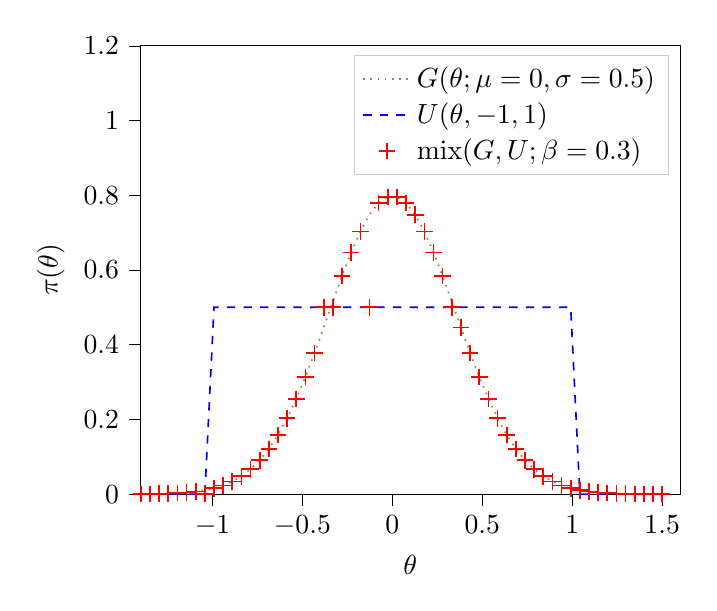
\begin{tikzpicture}

\begin{axis}[
legend cell align={left},
legend style={fill opacity=0.8, draw opacity=1, text opacity=1, draw=white!80!black},
tick align=outside,
tick pos=left,
x grid style={white!69.0196078431373!black},
xlabel={\(\displaystyle \theta\)},
xmin=-1.4, xmax=1.6,
xtick style={color=black},
y grid style={white!69.0196078431373!black},
ylabel={\(\displaystyle \pi(\theta)\)},
ymin=0, ymax=1.2,
ytick style={color=black}
]
\addplot [semithick, yellow!50!black, dotted]
table {%
-1.5 9.8466777332468e-05
-1.44915254237288 0.0001793872435764
-1.39830508474576 0.000320118348094559
-1.34745762711864 0.000559560121531124
-1.29661016949153 0.000958076356441112
-1.24576271186441 0.00160683272401611
-1.19491525423729 0.00263972321036136
-1.14406779661017 0.00424779248787262
-1.09322033898305 0.00669553635076534
-1.04237288135593 0.0103377167883577
-0.991525423728814 0.015634394496712
-0.940677966101695 0.0231608599466659
-0.889830508474576 0.0336082170150122
-0.838983050847458 0.0477698022564135
-0.788135593220339 0.066508720415643
-0.73728813559322 0.0907028470877726
-0.686440677966102 0.121165903387615
-0.635593220338983 0.15854666388776
-0.584745762711864 0.203212757823817
-0.533898305084746 0.255130282294824
-0.483050847457627 0.313754690902936
-0.432203389830508 0.377951108859794
-0.38135593220339 0.445962353038858
-0.330508474576271 0.515439801267037
-0.279661016949152 0.583545711433813
-0.228813559322034 0.647126211028834
-0.177966101694915 0.702943270974129
-0.127118644067796 0.747943415704262
-0.0762711864406778 0.77953278826435
-0.0254237288135593 0.795824323519198
0.0254237288135595 0.795824323519198
0.076271186440678 0.77953278826435
0.127118644067797 0.747943415704262
0.177966101694915 0.702943270974129
0.228813559322034 0.647126211028834
0.279661016949153 0.583545711433812
0.330508474576271 0.515439801267037
0.38135593220339 0.445962353038858
0.432203389830509 0.377951108859794
0.483050847457627 0.313754690902936
0.533898305084746 0.255130282294824
0.584745762711865 0.203212757823817
0.635593220338983 0.15854666388776
0.686440677966102 0.121165903387615
0.737288135593221 0.0907028470877724
0.788135593220339 0.0665087204156429
0.838983050847458 0.0477698022564135
0.889830508474577 0.0336082170150121
0.940677966101695 0.0231608599466659
0.991525423728814 0.015634394496712
1.04237288135593 0.0103377167883577
1.09322033898305 0.00669553635076532
1.14406779661017 0.00424779248787262
1.19491525423729 0.00263972321036135
1.24576271186441 0.0016068327240161
1.29661016949153 0.000958076356441112
1.34745762711864 0.000559560121531121
1.39830508474576 0.000320118348094558
1.44915254237288 0.000179387243576399
1.5 9.8466777332468e-05
};
\addlegendentry{$G(\theta; \mu=0, \sigma=0.5)$}
\addplot [semithick, blue, dashed]
table {%
-1.5 0
-1.44915254237288 0
-1.39830508474576 0
-1.34745762711864 0
-1.29661016949153 0
-1.24576271186441 0
-1.19491525423729 0
-1.14406779661017 0
-1.09322033898305 0
-1.04237288135593 0
-0.991525423728814 0.5
-0.940677966101695 0.5
-0.889830508474576 0.5
-0.838983050847458 0.5
-0.788135593220339 0.5
-0.73728813559322 0.5
-0.686440677966102 0.5
-0.635593220338983 0.5
-0.584745762711864 0.5
-0.533898305084746 0.5
-0.483050847457627 0.5
-0.432203389830508 0.5
-0.38135593220339 0.5
-0.330508474576271 0.5
-0.279661016949152 0.5
-0.228813559322034 0.5
-0.177966101694915 0.5
-0.127118644067796 0.5
-0.0762711864406778 0.5
-0.0254237288135593 0.5
0.0254237288135595 0.5
0.076271186440678 0.5
0.127118644067797 0.5
0.177966101694915 0.5
0.228813559322034 0.5
0.279661016949153 0.5
0.330508474576271 0.5
0.38135593220339 0.5
0.432203389830509 0.5
0.483050847457627 0.5
0.533898305084746 0.5
0.584745762711865 0.5
0.635593220338983 0.5
0.686440677966102 0.5
0.737288135593221 0.5
0.788135593220339 0.5
0.838983050847458 0.5
0.889830508474577 0.5
0.940677966101695 0.5
0.991525423728814 0.5
1.04237288135593 0
1.09322033898305 0
1.14406779661017 0
1.19491525423729 0
1.24576271186441 0
1.29661016949153 0
1.34745762711864 0
1.39830508474576 0
1.44915254237288 0
1.5 0
};
\addlegendentry{$U(\theta, -1, 1)$}
\addplot [semithick, red, mark=+, mark size=3, mark options={solid}, only marks]
table {%
-1.5 9.8466777332468e-05
-1.44915254237288 0.0001793872435764
-1.39830508474576 0
-1.34745762711864 0.000559560121531124
-1.29661016949153 0.000958076356441112
-1.24576271186441 0.00160683272401611
-1.19491525423729 0.00263972321036136
-1.14406779661017 0.00424779248787262
-1.09322033898305 0.00669553635076534
-1.04237288135593 0
-0.991525423728814 0.015634394496712
-0.940677966101695 0.0231608599466659
-0.889830508474576 0.0336082170150122
-0.838983050847458 0.0477698022564135
-0.788135593220339 0.066508720415643
-0.73728813559322 0.0907028470877726
-0.686440677966102 0.121165903387615
-0.635593220338983 0.15854666388776
-0.584745762711864 0.203212757823817
-0.533898305084746 0.255130282294824
-0.483050847457627 0.313754690902936
-0.432203389830508 0.377951108859794
-0.38135593220339 0.5
-0.330508474576271 0.5
-0.279661016949152 0.583545711433813
-0.228813559322034 0.647126211028834
-0.177966101694915 0.702943270974129
-0.127118644067796 0.5
-0.0762711864406778 0.77953278826435
-0.0254237288135593 0.795824323519198
0.0254237288135595 0.795824323519198
0.076271186440678 0.77953278826435
0.127118644067797 0.747943415704262
0.177966101694915 0.702943270974129
0.228813559322034 0.647126211028834
0.279661016949153 0.583545711433812
0.330508474576271 0.5
0.38135593220339 0.445962353038858
0.432203389830509 0.377951108859794
0.483050847457627 0.313754690902936
0.533898305084746 0.255130282294824
0.584745762711865 0.203212757823817
0.635593220338983 0.15854666388776
0.686440677966102 0.121165903387615
0.737288135593221 0.0907028470877724
0.788135593220339 0.0665087204156429
0.838983050847458 0.0477698022564135
0.889830508474577 0.0336082170150121
0.940677966101695 0.0231608599466659
0.991525423728814 0.015634394496712
1.04237288135593 0.0103377167883577
1.09322033898305 0.00669553635076532
1.14406779661017 0.00424779248787262
1.19491525423729 0.00263972321036135
1.24576271186441 0.0016068327240161
1.29661016949153 0.000958076356441112
1.34745762711864 0.000559560121531121
1.39830508474576 0.000320118348094558
1.44915254237288 0.000179387243576399
1.5 9.8466777332468e-05
};
\addlegendentry{mix$(G, U; \beta=0.3)$}
\end{axis}

\end{tikzpicture}

\caption{An example of a mixture repartitioning. Notice that the mixture is not normalised to emphasise the coincidence of values with both the uniform distribution and a Gaussian.\label{fig:mixture}}
\end{figure}



\section{Practical measurements}
\subsection{Performance}
We shall adopt the weighted accounting approach, which common in
computer science, to measure performance using the number of
\({\cal L}\) evaluations as the unit. Additionally, the
Kullback-Leibler divergence \({\cal D}\)~\cite[see]{Kullback_1951} is
used to estimate both the speed and the agreement of posteriors. It
defines an ordering on distributions: it's less for similar
distributions, ${\cal D}=0$ if identical everywhere in their domain.

\begin{figure}
  % This file was created by tikzplotlib v0.9.1.
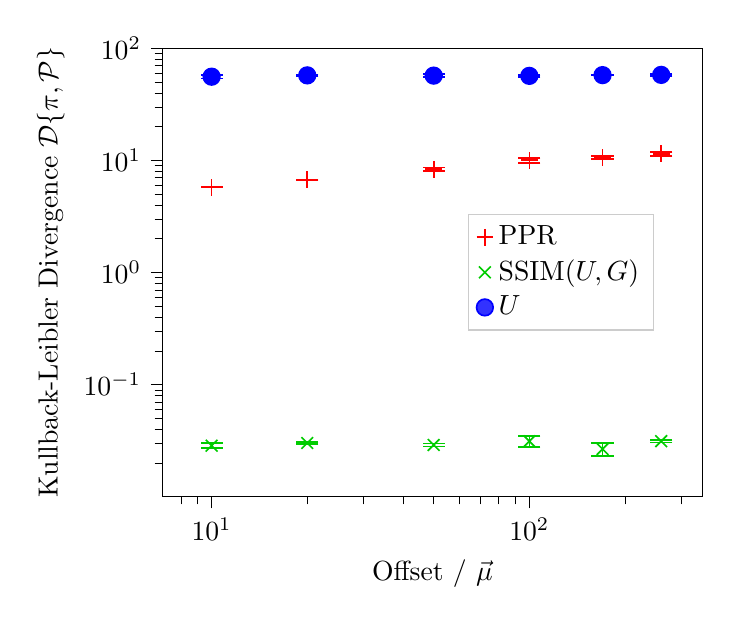
\begin{tikzpicture}

\definecolor{color0}{rgb}{1,0.0,0.0} %ppr
\definecolor{color1}{rgb}{0,0.8,0.0} %mix
\definecolor{color2}{rgb}{0.0,0.0,1.0} %U

\begin{axis}[
legend cell align={left},
legend style={fill opacity=0.8, draw opacity=1, text opacity=1, at={(0.91,0.5)}, anchor=east, draw=white!80!black},
tick align=outside,
tick pos=left,
x grid style={white!69.0196078431373!black},
xlabel={Offset / \(\displaystyle \vec{\mu}\)},
xmin=-3.0, xmax=350.0,
xtick style={color=black},
y grid style={white!69.0196078431373!black},
ylabel={Kullback-Leibler Divergence \(\displaystyle {\cal D}\{\pi, {\cal P}\}\)},
ymin=-3.0, ymax=100.0,
ytick style={color=black},
xmode=log,
ymode=log
]
\path [draw=color0, semithick]
(axis cs:10,5.71795365099151)
--(axis cs:10,5.77133948534581);

\path [draw=color0, semithick]
(axis cs:20,6.6768824419002)
--(axis cs:20,6.77321107556694);

\path [draw=color0, semithick]
(axis cs:50,8.02877279045042)
--(axis cs:50,8.63543918622054);

\path [draw=color0, semithick]
(axis cs:100,9.52185212376919)
--(axis cs:100,10.4908349952443);

\path [draw=color0, semithick]
(axis cs:170,10.3029683750536)
--(axis cs:170,10.9155451202318);

\path [draw=color0, semithick]
(axis cs:260,10.954510866509)
--(axis cs:260,11.9335782130671);

\path [draw=color1, semithick]
(axis cs:10,0.0271909650803472)
--(axis cs:10,0.030089733601838);

\path [draw=color1, semithick]
(axis cs:20,0.029683008672791)
--(axis cs:20,0.0308036500189849);

\path [draw=color1, semithick]
(axis cs:50,0.0282101242046804)
--(axis cs:50,0.0298855157628486);

\path [draw=color1, semithick]
(axis cs:100,0.0278177027329167)
--(axis cs:100,0.0348526563256524);

\path [draw=color1, semithick]
(axis cs:170,0.0232802581598788)
--(axis cs:170,0.0301604324600733);

\path [draw=color1, semithick]
(axis cs:260,0.0304771056975755)
--(axis cs:260,0.0323746358923458);

\path [draw=color2, semithick]
(axis cs:10,53.6407046096139)
--(axis cs:10,57.7293889288474);

\path [draw=color2, semithick]
(axis cs:20,56.1280894679801)
--(axis cs:20,58.3022565457241);

\path [draw=color2, semithick]
(axis cs:50,55.3633380690649)
--(axis cs:50,58.47445725549);

\path [draw=color2, semithick]
(axis cs:100,55.5223746731559)
--(axis cs:100,57.7271641567295);

\path [draw=color2, semithick]
(axis cs:170,56.8924880373743)
--(axis cs:170,58.1261131182599);

\path [draw=color2, semithick]
(axis cs:260,56.3603430284318)
--(axis cs:260,59.2024246504929);

\addplot [semithick, color0, mark=-, mark size=4, mark options={solid}, only marks, forget plot]
table {%
10 5.71795365099151
20 6.6768824419002
50 8.02877279045042
100 9.52185212376919
170 10.3029683750536
260 10.954510866509
};
\addplot [semithick, color0, mark=-, mark size=4, mark options={solid}, only marks, forget plot]
table {%
10 5.77133948534581
20 6.77321107556694
50 8.63543918622054
100 10.4908349952443
170 10.9155451202318
260 11.9335782130671
};
\addplot [semithick, color1, mark=-, mark size=4, mark options={solid}, only marks, forget plot]
table {%
10 0.0271909650803472
20 0.029683008672791
50 0.0282101242046804
100 0.0278177027329167
170 0.0232802581598788
260 0.0304771056975755
};
\addplot [semithick, color1, mark=-, mark size=4, mark options={solid}, only marks, forget plot]
table {%
10 0.030089733601838
20 0.0308036500189849
50 0.0298855157628486
100 0.0348526563256524
170 0.0301604324600733
260 0.0323746358923458
};
\addplot [semithick, color2, mark=-, mark size=4, mark options={solid}, only marks, forget plot]
table {%
10 53.6407046096139
20 56.1280894679801
50 55.3633380690649
100 55.5223746731559
170 56.8924880373743
260 56.3603430284318
};
\addplot [semithick, color2, mark=-, mark size=4, mark options={solid}, only marks, forget plot]
table {%
10 57.7293889288474
20 58.3022565457241
50 58.47445725549
100 57.7271641567295
170 58.1261131182599
260 59.2024246504929
};
\addplot [semithick, color0, mark=+, mark size=3, mark options={solid}, only marks]
table {%
10 5.74464656816866
20 6.72504675873357
50 8.33210598833548
100 10.0063435595067
170 10.6092567476427
260 11.4440445397881
};
\addlegendentry{PPR}
\addplot [semithick, color1, mark=x, mark size=3, mark options={solid}, only marks]
table {%
10 0.0286403493410926
20 0.0302433293458879
50 0.0290478199837645
100 0.0313351795292845
170 0.026720345309976
260 0.0314258707949607
};
\addlegendentry{SSIM$(U,G)$}
\addplot [semithick, color2, mark=*, mark size=3, mark options={solid}, only marks]
table {%
10 55.6850467692306
20 57.2151730068521
50 56.9188976622774
100 56.6247694149427
170 57.5093005778171
260 57.7813838394624
};
\addlegendentry{$U$}
\end{axis}

\end{tikzpicture}

\caption{Kullback-Leibler divergence \({\cal D}\) for different offsets: Gaussian peaks displaced from \(\bm{\mu}\) by \(\text{Offset}\times \bm{\mu}\). Notice that the faster repartitioning methods produce a lower value of \({\cal D}\). The divergence \({\cal D}\) scales linearly with the offset.\label{fig:kl-d}}
\end{figure}

\begin{figure}
  % This file was created by tikzplotlib v0.9.1.
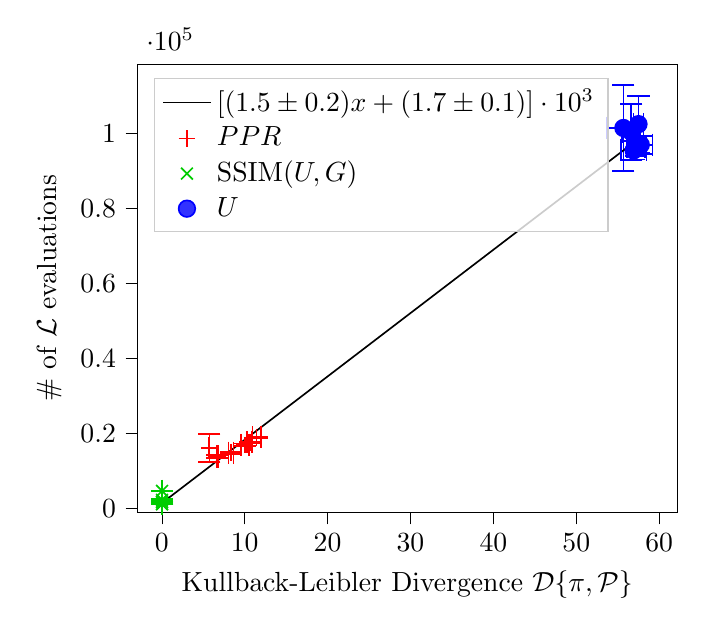
\begin{tikzpicture}

\definecolor{color0}{rgb}{1,0.0,0.0}
\definecolor{color1}{rgb}{0,0.8,0.0}
\definecolor{color2}{rgb}{0.0,0.0,1}
\definecolor{color3}{rgb}{0.0,0.0,0.0}

\begin{axis}[
legend cell align={left},
legend style={fill opacity=0.8, draw opacity=1, text opacity=1, at={(0.03,0.97)}, anchor=north west, draw=white!80!black},
tick align=outside,
tick pos=left,
x grid style={white!69.0196078431373!black},
xlabel={Kullback-Leibler Divergence \(\displaystyle {\cal D} \{\pi, {\cal P}\}\)},
xmin=-2.93567696145677, xmax=62.1613818701095,
xtick style={color=black},
y grid style={white!69.0196078431373!black},
ylabel={\# of \({\cal L}\) evaluations},
ymin=-1000.00, ymax=118545.85,
ytick style={color=black}
% ymode=log
]
\path [draw=color0, semithick]
(axis cs:5.71795365099151,16157.5)
--(axis cs:5.77133948534581,16157.5);

\path [draw=color0, semithick]
(axis cs:6.6768824419002,13953)
--(axis cs:6.77321107556694,13953);

\path [draw=color0, semithick]
(axis cs:8.02877279045042,14940.5)
--(axis cs:8.63543918622054,14940.5);

\path [draw=color0, semithick]
(axis cs:9.52185212376919,17043)
--(axis cs:10.4908349952443,17043);

\path [draw=color0, semithick]
(axis cs:10.3029683750536,17720.5)
--(axis cs:10.9155451202318,17720.5);

\path [draw=color0, semithick]
(axis cs:10.954510866509,19064.5)
--(axis cs:11.9335782130671,19064.5);

\path [draw=color0, semithick]
(axis cs:5.74464656816866,12446)
--(axis cs:5.74464656816866,19869);

\path [draw=color0, semithick]
(axis cs:6.72504675873357,13488)
--(axis cs:6.72504675873357,14418);

\path [draw=color0, semithick]
(axis cs:8.33210598833548,14689)
--(axis cs:8.33210598833548,15192);

\path [draw=color0, semithick]
(axis cs:10.0063435595067,16676)
--(axis cs:10.0063435595067,17410);

\path [draw=color0, semithick]
(axis cs:10.6092567476427,17618)
--(axis cs:10.6092567476427,17823);

\path [draw=color0, semithick]
(axis cs:11.4440445397881,18822)
--(axis cs:11.4440445397881,19307);

\path [draw=color1, semithick]
(axis cs:0.0271909650803472,2382.5)
--(axis cs:0.030089733601838,2382.5);

\path [draw=color1, semithick]
(axis cs:0.029683008672791,1207.5)
--(axis cs:0.0308036500189849,1207.5);

\path [draw=color1, semithick]
(axis cs:0.0282101242046804,1738.5)
--(axis cs:0.0298855157628486,1738.5);

\path [draw=color1, semithick]
(axis cs:0.0278177027329167,4757)
--(axis cs:0.0348526563256524,4757);

\path [draw=color1, semithick]
(axis cs:0.0232802581598788,1829.5)
--(axis cs:0.0301604324600733,1829.5);

\path [draw=color1, semithick]
(axis cs:0.0304771056975755,1224)
--(axis cs:0.0323746358923458,1224);

\path [draw=color1, semithick]
(axis cs:0.0286403493410926,2120)
--(axis cs:0.0286403493410926,2645);

\path [draw=color1, semithick]
(axis cs:0.0302433293458879,1163)
--(axis cs:0.0302433293458879,1252);

\path [draw=color1, semithick]
(axis cs:0.0290478199837645,1565)
--(axis cs:0.0290478199837645,1912);

\path [draw=color1, semithick]
(axis cs:0.0313351795292845,4698)
--(axis cs:0.0313351795292845,4816);

\path [draw=color1, semithick]
(axis cs:0.026720345309976,1740)
--(axis cs:0.026720345309976,1919);

\path [draw=color1, semithick]
(axis cs:0.0314258707949607,1138)
--(axis cs:0.0314258707949607,1310);

\path [draw=color2, semithick]
(axis cs:53.6407046096139,101541)
--(axis cs:57.7293889288474,101541);

\path [draw=color2, semithick]
(axis cs:56.1280894679801,96497)
--(axis cs:58.3022565457241,96497);

\path [draw=color2, semithick]
(axis cs:55.3633380690649,95565)
--(axis cs:58.47445725549,95565);

\path [draw=color2, semithick]
(axis cs:55.5223746731559,100523.5)
--(axis cs:57.7271641567295,100523.5);

\path [draw=color2, semithick]
(axis cs:56.8924880373743,102562.5)
--(axis cs:58.1261131182599,102562.5);

\path [draw=color2, semithick]
(axis cs:56.3603430284318,97066.5)
--(axis cs:59.2024246504929,97066.5);

\path [draw=color2, semithick]
(axis cs:55.6850467692306,90127)
--(axis cs:55.6850467692306,112955);

\path [draw=color2, semithick]
(axis cs:57.2151730068521,94020)
--(axis cs:57.2151730068521,98974);

\path [draw=color2, semithick]
(axis cs:56.9188976622774,93149)
--(axis cs:56.9188976622774,97981);

\path [draw=color2, semithick]
(axis cs:56.6247694149427,93079)
--(axis cs:56.6247694149427,107968);

\path [draw=color2, semithick]
(axis cs:57.5093005778171,94974)
--(axis cs:57.5093005778171,110151);

\path [draw=color2, semithick]
(axis cs:57.7813838394624,94657)
--(axis cs:57.7813838394624,99476);

\addplot [semithick, color0, mark=|, mark size=4, mark options={solid}, only marks, forget plot]
table {%
5.71795365099151 16157.5
6.6768824419002 13953
8.02877279045042 14940.5
9.52185212376919 17043
10.3029683750536 17720.5
10.954510866509 19064.5
};
\addplot [semithick, color0, mark=|, mark size=4, mark options={solid}, only marks, forget plot]
table {%
5.77133948534581 16157.5
6.77321107556694 13953
8.63543918622054 14940.5
10.4908349952443 17043
10.9155451202318 17720.5
11.9335782130671 19064.5
};
\addplot [semithick, color0, mark=-, mark size=4, mark options={solid}, only marks, forget plot]
table {%
5.74464656816866 12446
6.72504675873357 13488
8.33210598833548 14689
10.0063435595067 16676
10.6092567476427 17618
11.4440445397881 18822
};
\addplot [semithick, color0, mark=-, mark size=4, mark options={solid}, only marks, forget plot]
table {%
5.74464656816866 19869
6.72504675873357 14418
8.33210598833548 15192
10.0063435595067 17410
10.6092567476427 17823
11.4440445397881 19307
};
\addplot [semithick, color1, mark=|, mark size=4, mark options={solid}, only marks, forget plot]
table {%
0.0271909650803472 2382.5
0.029683008672791 1207.5
0.0282101242046804 1738.5
0.0278177027329167 4757
0.0232802581598788 1829.5
0.0304771056975755 1224
};
\addplot [semithick, color1, mark=|, mark size=4, mark options={solid}, only marks, forget plot]
table {%
0.030089733601838 2382.5
0.0308036500189849 1207.5
0.0298855157628486 1738.5
0.0348526563256524 4757
0.0301604324600733 1829.5
0.0323746358923458 1224
};
\addplot [semithick, color1, mark=-, mark size=4, mark options={solid}, only marks, forget plot]
table {%
0.0286403493410926 2120
0.0302433293458879 1163
0.0290478199837645 1565
0.0313351795292845 4698
0.026720345309976 1740
0.0314258707949607 1138
};
\addplot [semithick, color1, mark=-, mark size=4, mark options={solid}, only marks, forget plot]
table {%
0.0286403493410926 2645
0.0302433293458879 1252
0.0290478199837645 1912
0.0313351795292845 4816
0.026720345309976 1919
0.0314258707949607 1310
};
\addplot [semithick, color2, mark=|, mark size=4, mark options={solid}, only marks, forget plot]
table {%
53.6407046096139 101541
56.1280894679801 96497
55.3633380690649 95565
55.5223746731559 100523.5
56.8924880373743 102562.5
56.3603430284318 97066.5
};
\addplot [semithick, color2, mark=|, mark size=4, mark options={solid}, only marks, forget plot]
table {%
57.7293889288474 101541
58.3022565457241 96497
58.47445725549 95565
57.7271641567295 100523.5
58.1261131182599 102562.5
59.2024246504929 97066.5
};
\addplot [semithick, color2, mark=-, mark size=4, mark options={solid}, only marks, forget plot]
table {%
55.6850467692306 90127
57.2151730068521 94020
56.9188976622774 93149
56.6247694149427 93079
57.5093005778171 94974
57.7813838394624 94657
};
\addplot [semithick, color2, mark=-, mark size=4, mark options={solid}, only marks, forget plot]
table {%
55.6850467692306 112955
57.2151730068521 98974
56.9188976622774 97981
56.6247694149427 107968
57.5093005778171 110151
57.7813838394624 99476
};
\addplot [semithick, color3]
table {%
0.026720345309976 1539.88164299791
0.610100784644849 2525.39064984014
1.19348122397972 3510.89965668237
1.77686166331459 4496.4086635246
2.36024210264947 5481.91767036683
2.94362254198434 6467.42667720906
3.52700298131921 7452.93568405129
4.11038342065408 8438.44469089352
4.69376385998896 9423.95369773575
5.27714429932383 10409.462704578
5.8605247386587 11394.9717114202
6.44390517799357 12380.4807182624
7.02728561732845 13365.9897251047
7.61066605666332 14351.4987319469
8.19404649599819 15337.0077387891
8.77742693533306 16322.5167456314
9.36080737466794 17308.0257524736
9.94418781400281 18293.5347593158
10.5275682533377 19279.043766158
11.1109486926726 20264.5527730003
11.6943291320074 21250.0617798425
12.2777095713423 22235.5707866847
12.8610900106772 23221.079793527
13.444470450012 24206.5888003692
14.0278508893469 25192.0978072114
14.6112313286818 26177.6068140537
15.1946117680167 27163.1158208959
15.7779922073515 28148.6248277381
16.3613726466864 29134.1338345803
16.9447530860213 30119.6428414226
17.5281335253562 31105.1518482648
18.111513964691 32090.660855107
18.6948944040259 33076.1698619493
19.2782748433608 34061.6788687915
19.8616552826956 35047.1878756337
20.4450357220305 36032.6968824759
21.0284161613654 37018.2058893182
21.6117966007003 38003.7148961604
22.1951770400351 38989.2239030026
22.77855747937 39974.7329098449
23.3619379187049 40960.2419166871
23.9453183580397 41945.7509235293
24.5286987973746 42931.2599303716
25.1120792367095 43916.7689372138
25.6954596760444 44902.277944056
26.2788401153792 45887.7869508982
26.8622205547141 46873.2959577405
27.445600994049 47858.8049645827
28.0289814333839 48844.3139714249
28.6123618727187 49829.8229782672
29.1957423120536 50815.3319851094
29.7791227513885 51800.8409919516
30.3625031907233 52786.3499987938
30.9458836300582 53771.8590056361
31.5292640693931 54757.3680124783
32.112644508728 55742.8770193205
32.6960249480628 56728.3860261628
33.2794053873977 57713.895033005
33.8627858267326 58699.4040398472
34.4461662660675 59684.9130466895
35.0295467054023 60670.4220535317
35.6129271447372 61655.9310603739
36.1963075840721 62641.4400672161
36.7796880234069 63626.9490740584
37.3630684627418 64612.4580809006
37.9464489020767 65597.9670877428
38.5298293414116 66583.4760945851
39.1132097807464 67568.9851014273
39.6965902200813 68554.4941082695
40.2799706594162 69540.0031151118
40.863351098751 70525.512121954
41.4467315380859 71511.0211287962
42.0301119774208 72496.5301356384
42.6134924167557 73482.0391424807
43.1968728560905 74467.5481493229
43.7802532954254 75453.0571561651
44.3636337347603 76438.5661630074
44.9470141740952 77424.0751698496
45.53039461343 78409.5841766918
46.1137750527649 79395.093183534
46.6971554920998 80380.6021903763
47.2805359314346 81366.1111972185
47.8639163707695 82351.6202040607
48.4472968101044 83337.129210903
49.0306772494393 84322.6382177452
49.6140576887741 85308.1472245874
50.197438128109 86293.6562314297
50.7808185674439 87279.1652382719
51.3641990067788 88264.6742451141
51.9475794461136 89250.1832519564
52.5309598854485 90235.6922587986
53.1143403247834 91221.2012656408
53.6977207641182 92206.710272483
54.2811012034531 93192.2192793253
54.864481642788 94177.7282861675
55.4478620821229 95163.2372930097
56.0312425214577 96148.746299852
56.6146229607926 97134.2553066942
57.1980034001275 98119.7643135364
57.7813838394624 99105.2733203786
};
\addlegendentry{\(\left[(1.5 \pm 0.2)x + (1.7 \pm 0.1)\right]\cdot  10^3 \)}
\addplot [semithick, color0, mark=+, mark size=3, mark options={solid}, only marks]
table {%
5.74464656816866 16157.5
6.72504675873357 13953
8.33210598833548 14940.5
10.0063435595067 17043
10.6092567476427 17720.5
11.4440445397881 19064.5
};
\addlegendentry{$PPR$}
\addplot [semithick, color1, mark=x, mark size=3, mark options={solid}, only marks]
table {%
0.0286403493410926 2382.5
0.0302433293458879 1207.5
0.0290478199837645 1738.5
0.0313351795292845 4757
0.026720345309976 1829.5
0.0314258707949607 1224
};
\addlegendentry{SSIM$(U,G)$}
\addplot [semithick, color2, mark=*, mark size=3, mark options={solid}, only marks]
table {%
55.6850467692306 101541
57.2151730068521 96497
56.9188976622774 95565
56.6247694149427 100523.5
57.5093005778171 102562.5
57.7813838394624 97066.5
};
\addlegendentry{$U$}
\end{axis}

\end{tikzpicture}

\caption{Scaling of number of likelihood calls as a function of Kullback-Leibler divergence \({\cal D}\). The best fit line indicates that \({\cal D}\) is a reliable performance indicator for \texttt{PolyChord}.\label{fig:kl-scaling}}
\end{figure}


\begin{figure}
% This file was created by tikzplotlib v0.9.1.
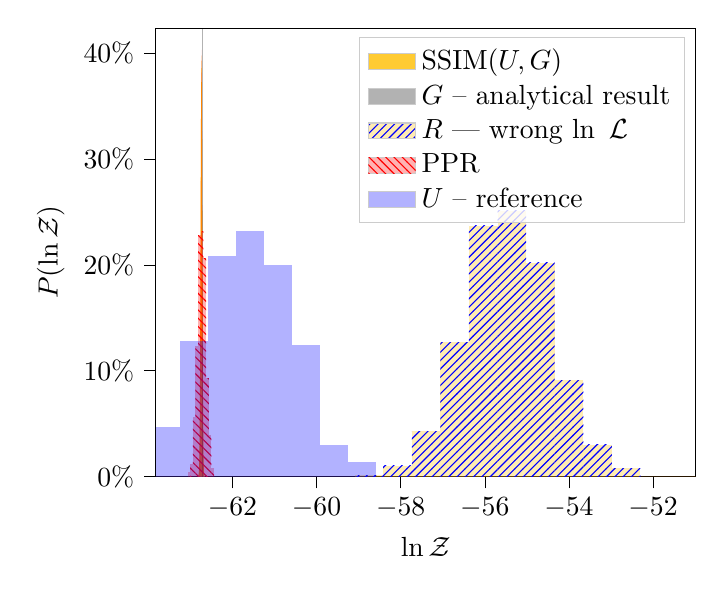
\begin{tikzpicture}

\definecolor{color2}{rgb}{0.0,0.0,1}
\definecolor{color1}{rgb}{1,0.00,0.00}
\definecolor{colorblack}{rgb}{0, 0, 0}
\definecolor{color0}{rgb}{1.0,0.75,0.0}

\begin{axis}[
legend cell align={left},
legend style={fill opacity=0.8, draw opacity=1, text opacity=1, anchor=north east, draw=white!80!black},
tick align=outside,
tick pos=left,
x grid style={white!69.0196078431373!black},
xlabel={\(\ln {\cal Z}\)},
xmin=-63.8198069562379, xmax=-50.9892026507015,
xtick style={color=black},
yticklabel={\pgfmathparse{\tick/10}\pgfmathprintnumber{\pgfmathresult}\%},
y grid style={white!69.0196078431373!black},
ylabel={\(P(\ln {\cal Z})\)},
ymin=0, ymax=423.473092744885,
ytick style={color=black}
]
\path [fill=color0]
(axis cs:-63.8198069562379,0)
--(axis cs:-63.8198069562379,0)
--(axis cs:-63.8069635084846,0)
--(axis cs:-63.7941200607313,0)
--(axis cs:-63.7812766129781,0)
--(axis cs:-63.7684331652248,0)
--(axis cs:-63.7555897174715,0)
--(axis cs:-63.7427462697182,0)
--(axis cs:-63.7299028219649,0)
--(axis cs:-63.7170593742116,0)
--(axis cs:-63.7042159264583,0)
--(axis cs:-63.691372478705,0)
--(axis cs:-63.6785290309517,0)
--(axis cs:-63.6656855831984,0)
--(axis cs:-63.6528421354452,0)
--(axis cs:-63.6399986876919,0)
--(axis cs:-63.6271552399386,0)
--(axis cs:-63.6143117921853,0)
--(axis cs:-63.601468344432,0)
--(axis cs:-63.5886248966787,0)
--(axis cs:-63.5757814489254,0)
--(axis cs:-63.5629380011721,0)
--(axis cs:-63.5500945534188,0)
--(axis cs:-63.5372511056656,0)
--(axis cs:-63.5244076579123,0)
--(axis cs:-63.511564210159,0)
--(axis cs:-63.4987207624057,0)
--(axis cs:-63.4858773146524,0)
--(axis cs:-63.4730338668991,0)
--(axis cs:-63.4601904191458,0)
--(axis cs:-63.4473469713925,0)
--(axis cs:-63.4345035236392,0)
--(axis cs:-63.4216600758859,0)
--(axis cs:-63.4088166281327,0)
--(axis cs:-63.3959731803794,0)
--(axis cs:-63.3831297326261,0)
--(axis cs:-63.3702862848728,0)
--(axis cs:-63.3574428371195,0)
--(axis cs:-63.3445993893662,0)
--(axis cs:-63.3317559416129,0)
--(axis cs:-63.3189124938596,0)
--(axis cs:-63.3060690461063,0)
--(axis cs:-63.293225598353,0)
--(axis cs:-63.2803821505998,0)
--(axis cs:-63.2675387028465,0)
--(axis cs:-63.2546952550932,0)
--(axis cs:-63.2418518073399,0)
--(axis cs:-63.2290083595866,0)
--(axis cs:-63.2161649118333,0)
--(axis cs:-63.20332146408,0)
--(axis cs:-63.1904780163267,0)
--(axis cs:-63.1776345685734,0)
--(axis cs:-63.1647911208201,0)
--(axis cs:-63.1519476730669,0)
--(axis cs:-63.1391042253136,0)
--(axis cs:-63.1262607775603,0)
--(axis cs:-63.113417329807,0)
--(axis cs:-63.1005738820537,0)
--(axis cs:-63.0877304343004,0)
--(axis cs:-63.0748869865471,0)
--(axis cs:-63.0620435387938,0)
--(axis cs:-63.0492000910405,0)
--(axis cs:-63.0363566432872,0)
--(axis cs:-63.023513195534,0)
--(axis cs:-63.0106697477807,0)
--(axis cs:-62.9978263000274,0)
--(axis cs:-62.9849828522741,0)
--(axis cs:-62.9721394045208,0)
--(axis cs:-62.9592959567675,0)
--(axis cs:-62.9464525090142,0)
--(axis cs:-62.9336090612609,0)
--(axis cs:-62.9207656135076,0)
--(axis cs:-62.9079221657544,0)
--(axis cs:-62.8950787180011,0)
--(axis cs:-62.8822352702478,0)
--(axis cs:-62.8693918224945,0)
--(axis cs:-62.8565483747412,0)
--(axis cs:-62.8437049269879,0)
--(axis cs:-62.8308614792346,0)
--(axis cs:-62.8180180314813,0)
--(axis cs:-62.805174583728,0)
--(axis cs:-62.7923311359747,0)
--(axis cs:-62.7794876882215,0)
--(axis cs:-62.7666442404682,0)
--(axis cs:-62.7538007927149,0)
--(axis cs:-62.7409573449616,0)
--(axis cs:-62.7281138972083,0)
--(axis cs:-62.715270449455,0)
--(axis cs:-62.7024270017017,0)
--(axis cs:-62.6895835539484,0)
--(axis cs:-62.6767401061951,0)
--(axis cs:-62.6638966584418,0)
--(axis cs:-62.6510532106886,0)
--(axis cs:-62.6382097629353,0)
--(axis cs:-62.625366315182,0)
--(axis cs:-62.6125228674287,0)
--(axis cs:-62.5996794196754,0)
--(axis cs:-62.5868359719221,0)
--(axis cs:-62.5739925241688,0)
--(axis cs:-62.5611490764155,0)
--(axis cs:-62.5483056286622,0)
--(axis cs:-62.535462180909,0)
--(axis cs:-62.5226187331557,0)
--(axis cs:-62.5097752854024,0)
--(axis cs:-62.4969318376491,0)
--(axis cs:-62.4840883898958,0)
--(axis cs:-62.4712449421425,0)
--(axis cs:-62.4584014943892,0)
--(axis cs:-62.4455580466359,0)
--(axis cs:-62.4327145988826,0)
--(axis cs:-62.4198711511293,0)
--(axis cs:-62.4070277033761,0)
--(axis cs:-62.3941842556228,0)
--(axis cs:-62.3813408078695,0)
--(axis cs:-62.3684973601162,0)
--(axis cs:-62.3556539123629,0)
--(axis cs:-62.3428104646096,0)
--(axis cs:-62.3299670168563,0)
--(axis cs:-62.317123569103,0)
--(axis cs:-62.3042801213497,0)
--(axis cs:-62.2914366735965,0)
--(axis cs:-62.2785932258432,0)
--(axis cs:-62.2657497780899,0)
--(axis cs:-62.2529063303366,0)
--(axis cs:-62.2400628825833,0)
--(axis cs:-62.22721943483,0)
--(axis cs:-62.2143759870767,0)
--(axis cs:-62.2015325393234,0)
--(axis cs:-62.1886890915701,0)
--(axis cs:-62.1758456438168,0)
--(axis cs:-62.1630021960636,0)
--(axis cs:-62.1501587483103,0)
--(axis cs:-62.137315300557,0)
--(axis cs:-62.1244718528037,0)
--(axis cs:-62.1116284050504,0)
--(axis cs:-62.0987849572971,0)
--(axis cs:-62.0859415095438,0)
--(axis cs:-62.0730980617905,0)
--(axis cs:-62.0602546140372,0)
--(axis cs:-62.0474111662839,0)
--(axis cs:-62.0345677185307,0)
--(axis cs:-62.0217242707774,0)
--(axis cs:-62.0088808230241,0)
--(axis cs:-61.9960373752708,0)
--(axis cs:-61.9831939275175,0)
--(axis cs:-61.9703504797642,0)
--(axis cs:-61.9575070320109,0)
--(axis cs:-61.9446635842576,0)
--(axis cs:-61.9318201365043,0)
--(axis cs:-61.918976688751,0)
--(axis cs:-61.9061332409978,0)
--(axis cs:-61.8932897932445,0)
--(axis cs:-61.8804463454912,0)
--(axis cs:-61.8676028977379,0)
--(axis cs:-61.8547594499846,0)
--(axis cs:-61.8419160022313,0)
--(axis cs:-61.829072554478,0)
--(axis cs:-61.8162291067247,0)
--(axis cs:-61.8033856589714,0)
--(axis cs:-61.7905422112181,0)
--(axis cs:-61.7776987634649,0)
--(axis cs:-61.7648553157116,0)
--(axis cs:-61.7520118679583,0)
--(axis cs:-61.739168420205,0)
--(axis cs:-61.7263249724517,0)
--(axis cs:-61.7134815246984,0)
--(axis cs:-61.7006380769451,0)
--(axis cs:-61.6877946291918,0)
--(axis cs:-61.6749511814385,0)
--(axis cs:-61.6621077336853,0)
--(axis cs:-61.649264285932,0)
--(axis cs:-61.6364208381787,0)
--(axis cs:-61.6235773904254,0)
--(axis cs:-61.6107339426721,0)
--(axis cs:-61.5978904949188,0)
--(axis cs:-61.5850470471655,0)
--(axis cs:-61.5722035994122,0)
--(axis cs:-61.5593601516589,0)
--(axis cs:-61.5465167039056,0)
--(axis cs:-61.5336732561524,0)
--(axis cs:-61.5208298083991,0)
--(axis cs:-61.5079863606458,0)
--(axis cs:-61.4951429128925,0)
--(axis cs:-61.4822994651392,0)
--(axis cs:-61.4694560173859,0)
--(axis cs:-61.4566125696326,0)
--(axis cs:-61.4437691218793,0)
--(axis cs:-61.430925674126,0)
--(axis cs:-61.4180822263727,0)
--(axis cs:-61.4052387786195,0)
--(axis cs:-61.3923953308662,0)
--(axis cs:-61.3795518831129,0)
--(axis cs:-61.3667084353596,0)
--(axis cs:-61.3538649876063,0)
--(axis cs:-61.341021539853,0)
--(axis cs:-61.3281780920997,0)
--(axis cs:-61.3153346443464,0)
--(axis cs:-61.3024911965931,0)
--(axis cs:-61.2896477488398,0)
--(axis cs:-61.2768043010866,0)
--(axis cs:-61.2639608533333,0)
--(axis cs:-61.25111740558,0)
--(axis cs:-61.2382739578267,0)
--(axis cs:-61.2254305100734,0)
--(axis cs:-61.2125870623201,0)
--(axis cs:-61.1997436145668,0)
--(axis cs:-61.1869001668135,0)
--(axis cs:-61.1740567190602,0)
--(axis cs:-61.1612132713069,0)
--(axis cs:-61.1483698235537,0)
--(axis cs:-61.1355263758004,0)
--(axis cs:-61.1226829280471,0)
--(axis cs:-61.1098394802938,0)
--(axis cs:-61.0969960325405,0)
--(axis cs:-61.0841525847872,0)
--(axis cs:-61.0713091370339,0)
--(axis cs:-61.0584656892806,0)
--(axis cs:-61.0456222415273,0)
--(axis cs:-61.0327787937741,0)
--(axis cs:-61.0199353460208,0)
--(axis cs:-61.0070918982675,0)
--(axis cs:-60.9942484505142,0)
--(axis cs:-60.9814050027609,0)
--(axis cs:-60.9685615550076,0)
--(axis cs:-60.9557181072543,0)
--(axis cs:-60.942874659501,0)
--(axis cs:-60.9300312117477,0)
--(axis cs:-60.9171877639944,0)
--(axis cs:-60.9043443162412,0)
--(axis cs:-60.8915008684879,0)
--(axis cs:-60.8786574207346,0)
--(axis cs:-60.8658139729813,0)
--(axis cs:-60.852970525228,0)
--(axis cs:-60.8401270774747,0)
--(axis cs:-60.8272836297214,0)
--(axis cs:-60.8144401819681,0)
--(axis cs:-60.8015967342148,0)
--(axis cs:-60.7887532864615,0)
--(axis cs:-60.7759098387083,0)
--(axis cs:-60.763066390955,0)
--(axis cs:-60.7502229432017,0)
--(axis cs:-60.7373794954484,0)
--(axis cs:-60.7245360476951,0)
--(axis cs:-60.7116925999418,0)
--(axis cs:-60.6988491521885,0)
--(axis cs:-60.6860057044352,0)
--(axis cs:-60.6731622566819,0)
--(axis cs:-60.6603188089287,0)
--(axis cs:-60.6474753611754,0)
--(axis cs:-60.6346319134221,0)
--(axis cs:-60.6217884656688,0)
--(axis cs:-60.6089450179155,0)
--(axis cs:-60.5961015701622,0)
--(axis cs:-60.5832581224089,0)
--(axis cs:-60.5704146746556,0)
--(axis cs:-60.5575712269023,0)
--(axis cs:-60.544727779149,0)
--(axis cs:-60.5318843313958,0)
--(axis cs:-60.5190408836425,0)
--(axis cs:-60.5061974358892,0)
--(axis cs:-60.4933539881359,0)
--(axis cs:-60.4805105403826,0)
--(axis cs:-60.4676670926293,0)
--(axis cs:-60.454823644876,0)
--(axis cs:-60.4419801971227,0)
--(axis cs:-60.4291367493694,0)
--(axis cs:-60.4162933016162,0)
--(axis cs:-60.4034498538629,0)
--(axis cs:-60.3906064061096,0)
--(axis cs:-60.3777629583563,0)
--(axis cs:-60.364919510603,0)
--(axis cs:-60.3520760628497,0)
--(axis cs:-60.3392326150964,0)
--(axis cs:-60.3263891673431,0)
--(axis cs:-60.3135457195898,0)
--(axis cs:-60.3007022718365,0)
--(axis cs:-60.2878588240833,0)
--(axis cs:-60.27501537633,0)
--(axis cs:-60.2621719285767,0)
--(axis cs:-60.2493284808234,0)
--(axis cs:-60.2364850330701,0)
--(axis cs:-60.2236415853168,0)
--(axis cs:-60.2107981375635,0)
--(axis cs:-60.1979546898102,0)
--(axis cs:-60.1851112420569,0)
--(axis cs:-60.1722677943036,0)
--(axis cs:-60.1594243465504,0)
--(axis cs:-60.1465808987971,0)
--(axis cs:-60.1337374510438,0)
--(axis cs:-60.1208940032905,0)
--(axis cs:-60.1080505555372,0)
--(axis cs:-60.0952071077839,0)
--(axis cs:-60.0823636600306,0)
--(axis cs:-60.0695202122773,0)
--(axis cs:-60.056676764524,0)
--(axis cs:-60.0438333167707,0)
--(axis cs:-60.0309898690175,0)
--(axis cs:-60.0181464212642,0)
--(axis cs:-60.0053029735109,0)
--(axis cs:-59.9924595257576,0)
--(axis cs:-59.9796160780043,0)
--(axis cs:-59.966772630251,0)
--(axis cs:-59.9539291824977,0)
--(axis cs:-59.9410857347444,0)
--(axis cs:-59.9282422869911,0)
--(axis cs:-59.9153988392378,0)
--(axis cs:-59.9025553914846,0)
--(axis cs:-59.8897119437313,0)
--(axis cs:-59.876868495978,0)
--(axis cs:-59.8640250482247,0)
--(axis cs:-59.8511816004714,0)
--(axis cs:-59.8383381527181,0)
--(axis cs:-59.8254947049648,0)
--(axis cs:-59.8126512572115,0)
--(axis cs:-59.7998078094582,0)
--(axis cs:-59.786964361705,0)
--(axis cs:-59.7741209139517,0)
--(axis cs:-59.7612774661984,0)
--(axis cs:-59.7484340184451,0)
--(axis cs:-59.7355905706918,0)
--(axis cs:-59.7227471229385,0)
--(axis cs:-59.7099036751852,0)
--(axis cs:-59.6970602274319,0)
--(axis cs:-59.6842167796786,0)
--(axis cs:-59.6713733319253,0)
--(axis cs:-59.6585298841721,0)
--(axis cs:-59.6456864364188,0)
--(axis cs:-59.6328429886655,0)
--(axis cs:-59.6199995409122,0)
--(axis cs:-59.6071560931589,0)
--(axis cs:-59.5943126454056,0)
--(axis cs:-59.5814691976523,0)
--(axis cs:-59.568625749899,0)
--(axis cs:-59.5557823021457,0)
--(axis cs:-59.5429388543924,0)
--(axis cs:-59.5300954066392,0)
--(axis cs:-59.5172519588859,0)
--(axis cs:-59.5044085111326,0)
--(axis cs:-59.4915650633793,0)
--(axis cs:-59.478721615626,0)
--(axis cs:-59.4658781678727,0)
--(axis cs:-59.4530347201194,0)
--(axis cs:-59.4401912723661,0)
--(axis cs:-59.4273478246128,0)
--(axis cs:-59.4145043768595,0)
--(axis cs:-59.4016609291063,0)
--(axis cs:-59.388817481353,0)
--(axis cs:-59.3759740335997,0)
--(axis cs:-59.3631305858464,0)
--(axis cs:-59.3502871380931,0)
--(axis cs:-59.3374436903398,0)
--(axis cs:-59.3246002425865,0)
--(axis cs:-59.3117567948332,0)
--(axis cs:-59.2989133470799,0)
--(axis cs:-59.2860698993266,0)
--(axis cs:-59.2732264515734,0)
--(axis cs:-59.2603830038201,0)
--(axis cs:-59.2475395560668,0)
--(axis cs:-59.2346961083135,0)
--(axis cs:-59.2218526605602,0)
--(axis cs:-59.2090092128069,0)
--(axis cs:-59.1961657650536,0)
--(axis cs:-59.1833223173003,0)
--(axis cs:-59.170478869547,0)
--(axis cs:-59.1576354217938,0)
--(axis cs:-59.1447919740405,0)
--(axis cs:-59.1319485262872,0)
--(axis cs:-59.1191050785339,0)
--(axis cs:-59.1062616307806,0)
--(axis cs:-59.0934181830273,0)
--(axis cs:-59.080574735274,0)
--(axis cs:-59.0677312875207,0)
--(axis cs:-59.0548878397674,0)
--(axis cs:-59.0420443920141,0)
--(axis cs:-59.0292009442609,0)
--(axis cs:-59.0163574965076,0)
--(axis cs:-59.0035140487543,0)
--(axis cs:-58.990670601001,0)
--(axis cs:-58.9778271532477,0)
--(axis cs:-58.9649837054944,0)
--(axis cs:-58.9521402577411,0)
--(axis cs:-58.9392968099878,0)
--(axis cs:-58.9264533622345,0)
--(axis cs:-58.9136099144812,0)
--(axis cs:-58.900766466728,0)
--(axis cs:-58.8879230189747,0)
--(axis cs:-58.8750795712214,0)
--(axis cs:-58.8622361234681,0)
--(axis cs:-58.8493926757148,0)
--(axis cs:-58.8365492279615,0)
--(axis cs:-58.8237057802082,0)
--(axis cs:-58.8108623324549,0)
--(axis cs:-58.7980188847016,0)
--(axis cs:-58.7851754369484,0)
--(axis cs:-58.7723319891951,0)
--(axis cs:-58.7594885414418,0)
--(axis cs:-58.7466450936885,0)
--(axis cs:-58.7338016459352,0)
--(axis cs:-58.7209581981819,0)
--(axis cs:-58.7081147504286,0)
--(axis cs:-58.6952713026753,0)
--(axis cs:-58.682427854922,0)
--(axis cs:-58.6695844071687,0)
--(axis cs:-58.6567409594155,0)
--(axis cs:-58.6438975116622,0)
--(axis cs:-58.6310540639089,0)
--(axis cs:-58.6182106161556,0)
--(axis cs:-58.6053671684023,0)
--(axis cs:-58.592523720649,0)
--(axis cs:-58.5796802728957,0)
--(axis cs:-58.5668368251424,0)
--(axis cs:-58.5539933773891,0)
--(axis cs:-58.5411499296358,0)
--(axis cs:-58.5283064818826,0)
--(axis cs:-58.5154630341293,0)
--(axis cs:-58.502619586376,0)
--(axis cs:-58.4897761386227,0)
--(axis cs:-58.4769326908694,0)
--(axis cs:-58.4640892431161,0)
--(axis cs:-58.4512457953628,0)
--(axis cs:-58.4384023476095,0)
--(axis cs:-58.4255588998562,0)
--(axis cs:-58.412715452103,0)
--(axis cs:-58.3998720043497,0)
--(axis cs:-58.3870285565964,0)
--(axis cs:-58.3741851088431,0)
--(axis cs:-58.3613416610898,0)
--(axis cs:-58.3484982133365,0)
--(axis cs:-58.3356547655832,0)
--(axis cs:-58.3228113178299,0)
--(axis cs:-58.3099678700766,0)
--(axis cs:-58.2971244223233,0)
--(axis cs:-58.2842809745701,0)
--(axis cs:-58.2714375268168,0)
--(axis cs:-58.2585940790635,0)
--(axis cs:-58.2457506313102,0)
--(axis cs:-58.2329071835569,0)
--(axis cs:-58.2200637358036,0)
--(axis cs:-58.2072202880503,0)
--(axis cs:-58.194376840297,0)
--(axis cs:-58.1815333925437,0)
--(axis cs:-58.1686899447904,0)
--(axis cs:-58.1558464970372,0)
--(axis cs:-58.1430030492839,0)
--(axis cs:-58.1301596015306,0)
--(axis cs:-58.1173161537773,0)
--(axis cs:-58.104472706024,0)
--(axis cs:-58.0916292582707,0)
--(axis cs:-58.0787858105174,0)
--(axis cs:-58.0659423627641,0)
--(axis cs:-58.0530989150108,0)
--(axis cs:-58.0402554672575,0)
--(axis cs:-58.0274120195043,0)
--(axis cs:-58.014568571751,0)
--(axis cs:-58.0017251239977,0)
--(axis cs:-57.9888816762444,0)
--(axis cs:-57.9760382284911,0)
--(axis cs:-57.9631947807378,0)
--(axis cs:-57.9503513329845,0)
--(axis cs:-57.9375078852312,0)
--(axis cs:-57.9246644374779,0)
--(axis cs:-57.9118209897247,0)
--(axis cs:-57.8989775419714,0)
--(axis cs:-57.8861340942181,0)
--(axis cs:-57.8732906464648,0)
--(axis cs:-57.8604471987115,0)
--(axis cs:-57.8476037509582,0)
--(axis cs:-57.8347603032049,0)
--(axis cs:-57.8219168554516,0)
--(axis cs:-57.8090734076983,0)
--(axis cs:-57.796229959945,0)
--(axis cs:-57.7833865121918,0)
--(axis cs:-57.7705430644385,0)
--(axis cs:-57.7576996166852,0)
--(axis cs:-57.7448561689319,0)
--(axis cs:-57.7320127211786,0)
--(axis cs:-57.7191692734253,0)
--(axis cs:-57.706325825672,0)
--(axis cs:-57.6934823779187,0)
--(axis cs:-57.6806389301654,0)
--(axis cs:-57.6677954824121,0)
--(axis cs:-57.6549520346589,0)
--(axis cs:-57.6421085869056,0)
--(axis cs:-57.6292651391523,0)
--(axis cs:-57.616421691399,0)
--(axis cs:-57.6035782436457,0)
--(axis cs:-57.5907347958924,0)
--(axis cs:-57.5778913481391,0)
--(axis cs:-57.5650479003858,0)
--(axis cs:-57.5522044526325,0)
--(axis cs:-57.5393610048792,0)
--(axis cs:-57.526517557126,0)
--(axis cs:-57.5136741093727,0)
--(axis cs:-57.5008306616194,0)
--(axis cs:-57.4879872138661,0)
--(axis cs:-57.4751437661128,0)
--(axis cs:-57.4623003183595,0)
--(axis cs:-57.4494568706062,0)
--(axis cs:-57.4366134228529,0)
--(axis cs:-57.4237699750996,0)
--(axis cs:-57.4109265273463,0)
--(axis cs:-57.3980830795931,0)
--(axis cs:-57.3852396318398,0)
--(axis cs:-57.3723961840865,0)
--(axis cs:-57.3595527363332,0)
--(axis cs:-57.3467092885799,0)
--(axis cs:-57.3338658408266,0)
--(axis cs:-57.3210223930733,0)
--(axis cs:-57.30817894532,0)
--(axis cs:-57.2953354975667,0)
--(axis cs:-57.2824920498135,0)
--(axis cs:-57.2696486020602,0)
--(axis cs:-57.2568051543069,0)
--(axis cs:-57.2439617065536,0)
--(axis cs:-57.2311182588003,0)
--(axis cs:-57.218274811047,0)
--(axis cs:-57.2054313632937,0)
--(axis cs:-57.1925879155404,0)
--(axis cs:-57.1797444677871,0)
--(axis cs:-57.1669010200338,0)
--(axis cs:-57.1540575722806,0)
--(axis cs:-57.1412141245273,0)
--(axis cs:-57.128370676774,0)
--(axis cs:-57.1155272290207,0)
--(axis cs:-57.1026837812674,0)
--(axis cs:-57.0898403335141,0)
--(axis cs:-57.0769968857608,0)
--(axis cs:-57.0641534380075,0)
--(axis cs:-57.0513099902542,0)
--(axis cs:-57.0384665425009,0)
--(axis cs:-57.0256230947477,0)
--(axis cs:-57.0127796469944,0)
--(axis cs:-56.9999361992411,0)
--(axis cs:-56.9870927514878,0)
--(axis cs:-56.9742493037345,0)
--(axis cs:-56.9614058559812,0)
--(axis cs:-56.9485624082279,0)
--(axis cs:-56.9357189604746,0)
--(axis cs:-56.9228755127213,0)
--(axis cs:-56.910032064968,0)
--(axis cs:-56.8971886172148,0)
--(axis cs:-56.8843451694615,0)
--(axis cs:-56.8715017217082,0)
--(axis cs:-56.8586582739549,0)
--(axis cs:-56.8458148262016,0)
--(axis cs:-56.8329713784483,0)
--(axis cs:-56.820127930695,0)
--(axis cs:-56.8072844829417,0)
--(axis cs:-56.7944410351884,0)
--(axis cs:-56.7815975874352,0)
--(axis cs:-56.7687541396819,0)
--(axis cs:-56.7559106919286,0)
--(axis cs:-56.7430672441753,0)
--(axis cs:-56.730223796422,0)
--(axis cs:-56.7173803486687,0)
--(axis cs:-56.7045369009154,0)
--(axis cs:-56.6916934531621,0)
--(axis cs:-56.6788500054088,0)
--(axis cs:-56.6660065576555,0)
--(axis cs:-56.6531631099023,0)
--(axis cs:-56.640319662149,0)
--(axis cs:-56.6274762143957,0)
--(axis cs:-56.6146327666424,0)
--(axis cs:-56.6017893188891,0)
--(axis cs:-56.5889458711358,0)
--(axis cs:-56.5761024233825,0)
--(axis cs:-56.5632589756292,0)
--(axis cs:-56.5504155278759,0)
--(axis cs:-56.5375720801227,0)
--(axis cs:-56.5247286323694,0)
--(axis cs:-56.5118851846161,0)
--(axis cs:-56.4990417368628,0)
--(axis cs:-56.4861982891095,0)
--(axis cs:-56.4733548413562,0)
--(axis cs:-56.4605113936029,0)
--(axis cs:-56.4476679458496,0)
--(axis cs:-56.4348244980963,0)
--(axis cs:-56.421981050343,0)
--(axis cs:-56.4091376025898,0)
--(axis cs:-56.3962941548365,0)
--(axis cs:-56.3834507070832,0)
--(axis cs:-56.3706072593299,0)
--(axis cs:-56.3577638115766,0)
--(axis cs:-56.3449203638233,0)
--(axis cs:-56.33207691607,0)
--(axis cs:-56.3192334683167,0)
--(axis cs:-56.3063900205634,0)
--(axis cs:-56.2935465728101,0)
--(axis cs:-56.2807031250569,0)
--(axis cs:-56.2678596773036,0)
--(axis cs:-56.2550162295503,0)
--(axis cs:-56.242172781797,0)
--(axis cs:-56.2293293340437,0)
--(axis cs:-56.2164858862904,0)
--(axis cs:-56.2036424385371,0)
--(axis cs:-56.1907989907838,0)
--(axis cs:-56.1779555430305,0)
--(axis cs:-56.1651120952772,0)
--(axis cs:-56.152268647524,0)
--(axis cs:-56.1394251997707,0)
--(axis cs:-56.1265817520174,0)
--(axis cs:-56.1137383042641,0)
--(axis cs:-56.1008948565108,0)
--(axis cs:-56.0880514087575,0)
--(axis cs:-56.0752079610042,0)
--(axis cs:-56.0623645132509,0)
--(axis cs:-56.0495210654976,0)
--(axis cs:-56.0366776177444,0)
--(axis cs:-56.0238341699911,0)
--(axis cs:-56.0109907222378,0)
--(axis cs:-55.9981472744845,0)
--(axis cs:-55.9853038267312,0)
--(axis cs:-55.9724603789779,0)
--(axis cs:-55.9596169312246,0)
--(axis cs:-55.9467734834713,0)
--(axis cs:-55.933930035718,0)
--(axis cs:-55.9210865879647,0)
--(axis cs:-55.9082431402115,0)
--(axis cs:-55.8953996924582,0)
--(axis cs:-55.8825562447049,0)
--(axis cs:-55.8697127969516,0)
--(axis cs:-55.8568693491983,0)
--(axis cs:-55.844025901445,0)
--(axis cs:-55.8311824536917,0)
--(axis cs:-55.8183390059384,0)
--(axis cs:-55.8054955581851,0)
--(axis cs:-55.7926521104318,0)
--(axis cs:-55.7798086626786,0)
--(axis cs:-55.7669652149253,0)
--(axis cs:-55.754121767172,0)
--(axis cs:-55.7412783194187,0)
--(axis cs:-55.7284348716654,0)
--(axis cs:-55.7155914239121,0)
--(axis cs:-55.7027479761588,0)
--(axis cs:-55.6899045284055,0)
--(axis cs:-55.6770610806522,0)
--(axis cs:-55.6642176328989,0)
--(axis cs:-55.6513741851457,0)
--(axis cs:-55.6385307373924,0)
--(axis cs:-55.6256872896391,0)
--(axis cs:-55.6128438418858,0)
--(axis cs:-55.6000003941325,0)
--(axis cs:-55.5871569463792,0)
--(axis cs:-55.5743134986259,0)
--(axis cs:-55.5614700508726,0)
--(axis cs:-55.5486266031193,0)
--(axis cs:-55.535783155366,0)
--(axis cs:-55.5229397076128,0)
--(axis cs:-55.5100962598595,0)
--(axis cs:-55.4972528121062,0)
--(axis cs:-55.4844093643529,0)
--(axis cs:-55.4715659165996,0)
--(axis cs:-55.4587224688463,0)
--(axis cs:-55.445879021093,0)
--(axis cs:-55.4330355733397,0)
--(axis cs:-55.4201921255864,0)
--(axis cs:-55.4073486778332,0)
--(axis cs:-55.3945052300799,0)
--(axis cs:-55.3816617823266,0)
--(axis cs:-55.3688183345733,0)
--(axis cs:-55.35597488682,0)
--(axis cs:-55.3431314390667,0)
--(axis cs:-55.3302879913134,0)
--(axis cs:-55.3174445435601,0)
--(axis cs:-55.3046010958068,0)
--(axis cs:-55.2917576480535,0)
--(axis cs:-55.2789142003003,0)
--(axis cs:-55.266070752547,0)
--(axis cs:-55.2532273047937,0)
--(axis cs:-55.2403838570404,0)
--(axis cs:-55.2275404092871,0)
--(axis cs:-55.2146969615338,0)
--(axis cs:-55.2018535137805,0)
--(axis cs:-55.1890100660272,0)
--(axis cs:-55.1761666182739,0)
--(axis cs:-55.1633231705206,0)
--(axis cs:-55.1504797227674,0)
--(axis cs:-55.1376362750141,0)
--(axis cs:-55.1247928272608,0)
--(axis cs:-55.1119493795075,0)
--(axis cs:-55.0991059317542,0)
--(axis cs:-55.0862624840009,0)
--(axis cs:-55.0734190362476,0)
--(axis cs:-55.0605755884943,0)
--(axis cs:-55.047732140741,0)
--(axis cs:-55.0348886929877,0)
--(axis cs:-55.0220452452345,0)
--(axis cs:-55.0092017974812,0)
--(axis cs:-54.9963583497279,0)
--(axis cs:-54.9835149019746,0)
--(axis cs:-54.9706714542213,0)
--(axis cs:-54.957828006468,0)
--(axis cs:-54.9449845587147,0)
--(axis cs:-54.9321411109614,0)
--(axis cs:-54.9192976632081,0)
--(axis cs:-54.9064542154549,0)
--(axis cs:-54.8936107677016,0)
--(axis cs:-54.8807673199483,0)
--(axis cs:-54.867923872195,0)
--(axis cs:-54.8550804244417,0)
--(axis cs:-54.8422369766884,0)
--(axis cs:-54.8293935289351,0)
--(axis cs:-54.8165500811818,0)
--(axis cs:-54.8037066334285,0)
--(axis cs:-54.7908631856752,0)
--(axis cs:-54.778019737922,0)
--(axis cs:-54.7651762901687,0)
--(axis cs:-54.7523328424154,0)
--(axis cs:-54.7394893946621,0)
--(axis cs:-54.7266459469088,0)
--(axis cs:-54.7138024991555,0)
--(axis cs:-54.7009590514022,0)
--(axis cs:-54.6881156036489,0)
--(axis cs:-54.6752721558956,0)
--(axis cs:-54.6624287081424,0)
--(axis cs:-54.6495852603891,0)
--(axis cs:-54.6367418126358,0)
--(axis cs:-54.6238983648825,0)
--(axis cs:-54.6110549171292,0)
--(axis cs:-54.5982114693759,0)
--(axis cs:-54.5853680216226,0)
--(axis cs:-54.5725245738693,0)
--(axis cs:-54.559681126116,0)
--(axis cs:-54.5468376783627,0)
--(axis cs:-54.5339942306095,0)
--(axis cs:-54.5211507828562,0)
--(axis cs:-54.5083073351029,0)
--(axis cs:-54.4954638873496,0)
--(axis cs:-54.4826204395963,0)
--(axis cs:-54.469776991843,0)
--(axis cs:-54.4569335440897,0)
--(axis cs:-54.4440900963364,0)
--(axis cs:-54.4312466485831,0)
--(axis cs:-54.4184032008298,0)
--(axis cs:-54.4055597530766,0)
--(axis cs:-54.3927163053233,0)
--(axis cs:-54.37987285757,0)
--(axis cs:-54.3670294098167,0)
--(axis cs:-54.3541859620634,0)
--(axis cs:-54.3413425143101,0)
--(axis cs:-54.3284990665568,0)
--(axis cs:-54.3156556188035,0)
--(axis cs:-54.3028121710502,0)
--(axis cs:-54.2899687232969,0)
--(axis cs:-54.2771252755437,0)
--(axis cs:-54.2642818277904,0)
--(axis cs:-54.2514383800371,0)
--(axis cs:-54.2385949322838,0)
--(axis cs:-54.2257514845305,0)
--(axis cs:-54.2129080367772,0)
--(axis cs:-54.2000645890239,0)
--(axis cs:-54.1872211412706,0)
--(axis cs:-54.1743776935173,0)
--(axis cs:-54.161534245764,0)
--(axis cs:-54.1486907980108,0)
--(axis cs:-54.1358473502575,0)
--(axis cs:-54.1230039025042,0)
--(axis cs:-54.1101604547509,0)
--(axis cs:-54.0973170069976,0)
--(axis cs:-54.0844735592443,0)
--(axis cs:-54.071630111491,0)
--(axis cs:-54.0587866637377,0)
--(axis cs:-54.0459432159844,0)
--(axis cs:-54.0330997682312,0)
--(axis cs:-54.0202563204779,0)
--(axis cs:-54.0074128727246,0)
--(axis cs:-53.9945694249713,0)
--(axis cs:-53.981725977218,0)
--(axis cs:-53.9688825294647,0)
--(axis cs:-53.9560390817114,0)
--(axis cs:-53.9431956339581,0)
--(axis cs:-53.9303521862048,0)
--(axis cs:-53.9175087384515,0)
--(axis cs:-53.9046652906983,0)
--(axis cs:-53.891821842945,0)
--(axis cs:-53.8789783951917,0)
--(axis cs:-53.8661349474384,0)
--(axis cs:-53.8532914996851,0)
--(axis cs:-53.8404480519318,0)
--(axis cs:-53.8276046041785,0)
--(axis cs:-53.8147611564252,0)
--(axis cs:-53.8019177086719,0)
--(axis cs:-53.7890742609186,0)
--(axis cs:-53.7762308131654,0)
--(axis cs:-53.7633873654121,0)
--(axis cs:-53.7505439176588,0)
--(axis cs:-53.7377004699055,0)
--(axis cs:-53.7248570221522,0)
--(axis cs:-53.7120135743989,0)
--(axis cs:-53.6991701266456,0)
--(axis cs:-53.6863266788923,0)
--(axis cs:-53.673483231139,0)
--(axis cs:-53.6606397833857,0)
--(axis cs:-53.6477963356325,0)
--(axis cs:-53.6349528878792,0)
--(axis cs:-53.6221094401259,0)
--(axis cs:-53.6092659923726,0)
--(axis cs:-53.5964225446193,0)
--(axis cs:-53.583579096866,0)
--(axis cs:-53.5707356491127,0)
--(axis cs:-53.5578922013594,0)
--(axis cs:-53.5450487536061,0)
--(axis cs:-53.5322053058529,0)
--(axis cs:-53.5193618580996,0)
--(axis cs:-53.5065184103463,0)
--(axis cs:-53.493674962593,0)
--(axis cs:-53.4808315148397,0)
--(axis cs:-53.4679880670864,0)
--(axis cs:-53.4551446193331,0)
--(axis cs:-53.4423011715798,0)
--(axis cs:-53.4294577238265,0)
--(axis cs:-53.4166142760732,0)
--(axis cs:-53.40377082832,0)
--(axis cs:-53.3909273805667,0)
--(axis cs:-53.3780839328134,0)
--(axis cs:-53.3652404850601,0)
--(axis cs:-53.3523970373068,0)
--(axis cs:-53.3395535895535,0)
--(axis cs:-53.3267101418002,0)
--(axis cs:-53.3138666940469,0)
--(axis cs:-53.3010232462936,0)
--(axis cs:-53.2881797985403,0)
--(axis cs:-53.2753363507871,0)
--(axis cs:-53.2624929030338,0)
--(axis cs:-53.2496494552805,0)
--(axis cs:-53.2368060075272,0)
--(axis cs:-53.2239625597739,0)
--(axis cs:-53.2111191120206,0)
--(axis cs:-53.1982756642673,0)
--(axis cs:-53.185432216514,0)
--(axis cs:-53.1725887687607,0)
--(axis cs:-53.1597453210074,0)
--(axis cs:-53.1469018732542,0)
--(axis cs:-53.1340584255009,0)
--(axis cs:-53.1212149777476,0)
--(axis cs:-53.1083715299943,0)
--(axis cs:-53.095528082241,0)
--(axis cs:-53.0826846344877,0)
--(axis cs:-53.0698411867344,0)
--(axis cs:-53.0569977389811,0)
--(axis cs:-53.0441542912278,0)
--(axis cs:-53.0313108434746,0)
--(axis cs:-53.0184673957213,0)
--(axis cs:-53.005623947968,0)
--(axis cs:-52.9927805002147,0)
--(axis cs:-52.9799370524614,0)
--(axis cs:-52.9670936047081,0)
--(axis cs:-52.9542501569548,0)
--(axis cs:-52.9414067092015,0)
--(axis cs:-52.9285632614482,0)
--(axis cs:-52.9157198136949,0)
--(axis cs:-52.9028763659417,0)
--(axis cs:-52.8900329181884,0)
--(axis cs:-52.8771894704351,0)
--(axis cs:-52.8643460226818,0)
--(axis cs:-52.8515025749285,0)
--(axis cs:-52.8386591271752,0)
--(axis cs:-52.8258156794219,0)
--(axis cs:-52.8129722316686,0)
--(axis cs:-52.8001287839153,0)
--(axis cs:-52.787285336162,0)
--(axis cs:-52.7744418884088,0)
--(axis cs:-52.7615984406555,0)
--(axis cs:-52.7487549929022,0)
--(axis cs:-52.7359115451489,0)
--(axis cs:-52.7230680973956,0)
--(axis cs:-52.7102246496423,0)
--(axis cs:-52.697381201889,0)
--(axis cs:-52.6845377541357,0)
--(axis cs:-52.6716943063824,0)
--(axis cs:-52.6588508586292,0)
--(axis cs:-52.6460074108759,0)
--(axis cs:-52.6331639631226,0)
--(axis cs:-52.6203205153693,0)
--(axis cs:-52.607477067616,0)
--(axis cs:-52.5946336198627,0)
--(axis cs:-52.5817901721094,0)
--(axis cs:-52.5689467243561,0)
--(axis cs:-52.5561032766028,0)
--(axis cs:-52.5432598288495,0)
--(axis cs:-52.5304163810963,0)
--(axis cs:-52.517572933343,0)
--(axis cs:-52.5047294855897,0)
--(axis cs:-52.4918860378364,0)
--(axis cs:-52.4790425900831,0)
--(axis cs:-52.4661991423298,0)
--(axis cs:-52.4533556945765,0)
--(axis cs:-52.4405122468232,0)
--(axis cs:-52.4276687990699,0)
--(axis cs:-52.4148253513166,0)
--(axis cs:-52.4019819035634,0)
--(axis cs:-52.3891384558101,0)
--(axis cs:-52.3762950080568,0)
--(axis cs:-52.3634515603035,0)
--(axis cs:-52.3506081125502,0)
--(axis cs:-52.3377646647969,0)
--(axis cs:-52.3249212170436,0)
--(axis cs:-52.3120777692903,0)
--(axis cs:-52.299234321537,0)
--(axis cs:-52.2863908737837,0)
--(axis cs:-52.2735474260305,0)
--(axis cs:-52.2607039782772,0)
--(axis cs:-52.2478605305239,0)
--(axis cs:-52.2350170827706,0)
--(axis cs:-52.2221736350173,0)
--(axis cs:-52.209330187264,0)
--(axis cs:-52.1964867395107,0)
--(axis cs:-52.1836432917574,0)
--(axis cs:-52.1707998440041,0)
--(axis cs:-52.1579563962509,0)
--(axis cs:-52.1451129484976,0)
--(axis cs:-52.1322695007443,0)
--(axis cs:-52.119426052991,0)
--(axis cs:-52.1065826052377,0)
--(axis cs:-52.0937391574844,0)
--(axis cs:-52.0808957097311,0)
--(axis cs:-52.0680522619778,0)
--(axis cs:-52.0552088142245,0)
--(axis cs:-52.0423653664712,0)
--(axis cs:-52.029521918718,0)
--(axis cs:-52.0166784709647,0)
--(axis cs:-52.0038350232114,0)
--(axis cs:-51.9909915754581,0)
--(axis cs:-51.9781481277048,0)
--(axis cs:-51.9653046799515,0)
--(axis cs:-51.9524612321982,0)
--(axis cs:-51.9396177844449,0)
--(axis cs:-51.9267743366916,0)
--(axis cs:-51.9139308889383,0)
--(axis cs:-51.9010874411851,0)
--(axis cs:-51.8882439934318,0)
--(axis cs:-51.8754005456785,0)
--(axis cs:-51.8625570979252,0)
--(axis cs:-51.8497136501719,0)
--(axis cs:-51.8368702024186,0)
--(axis cs:-51.8240267546653,0)
--(axis cs:-51.811183306912,0)
--(axis cs:-51.7983398591587,0)
--(axis cs:-51.7854964114054,0)
--(axis cs:-51.7726529636522,0)
--(axis cs:-51.7598095158989,0)
--(axis cs:-51.7469660681456,0)
--(axis cs:-51.7341226203923,0)
--(axis cs:-51.721279172639,0)
--(axis cs:-51.7084357248857,0)
--(axis cs:-51.6955922771324,0)
--(axis cs:-51.6827488293791,0)
--(axis cs:-51.6699053816258,0)
--(axis cs:-51.6570619338726,0)
--(axis cs:-51.6442184861193,0)
--(axis cs:-51.631375038366,0)
--(axis cs:-51.6185315906127,0)
--(axis cs:-51.6056881428594,0)
--(axis cs:-51.5928446951061,0)
--(axis cs:-51.5800012473528,0)
--(axis cs:-51.5671577995995,0)
--(axis cs:-51.5543143518462,0)
--(axis cs:-51.5414709040929,0)
--(axis cs:-51.5286274563397,0)
--(axis cs:-51.5157840085864,0)
--(axis cs:-51.5029405608331,0)
--(axis cs:-51.4900971130798,0)
--(axis cs:-51.4772536653265,0)
--(axis cs:-51.4644102175732,0)
--(axis cs:-51.4515667698199,0)
--(axis cs:-51.4387233220666,0)
--(axis cs:-51.4258798743133,0)
--(axis cs:-51.41303642656,0)
--(axis cs:-51.4001929788068,0)
--(axis cs:-51.3873495310535,0)
--(axis cs:-51.3745060833002,0)
--(axis cs:-51.3616626355469,0)
--(axis cs:-51.3488191877936,0)
--(axis cs:-51.3359757400403,0)
--(axis cs:-51.323132292287,0)
--(axis cs:-51.3102888445337,0)
--(axis cs:-51.2974453967804,0)
--(axis cs:-51.2846019490271,0)
--(axis cs:-51.2717585012739,0)
--(axis cs:-51.2589150535206,0)
--(axis cs:-51.2460716057673,0)
--(axis cs:-51.233228158014,0)
--(axis cs:-51.2203847102607,0)
--(axis cs:-51.2075412625074,0)
--(axis cs:-51.1946978147541,0)
--(axis cs:-51.1818543670008,0)
--(axis cs:-51.1690109192475,0)
--(axis cs:-51.1561674714942,0)
--(axis cs:-51.143324023741,0)
--(axis cs:-51.1304805759877,0)
--(axis cs:-51.1176371282344,0)
--(axis cs:-51.1047936804811,0)
--(axis cs:-51.0919502327278,0)
--(axis cs:-51.0791067849745,0)
--(axis cs:-51.0662633372212,0)
--(axis cs:-51.0534198894679,0)
--(axis cs:-51.0405764417146,0)
--(axis cs:-51.0277329939614,0)
--(axis cs:-51.0148895462081,0)
--(axis cs:-51.0020460984548,0)
--(axis cs:-50.9892026507015,0)
--(axis cs:-50.9892026507015,0)
--(axis cs:-50.9892026507015,0)
--(axis cs:-51.0020460984548,0)
--(axis cs:-51.0148895462081,0)
--(axis cs:-51.0277329939614,0)
--(axis cs:-51.0405764417146,0)
--(axis cs:-51.0534198894679,0)
--(axis cs:-51.0662633372212,0)
--(axis cs:-51.0791067849745,0)
--(axis cs:-51.0919502327278,0)
--(axis cs:-51.1047936804811,0)
--(axis cs:-51.1176371282344,0)
--(axis cs:-51.1304805759877,0)
--(axis cs:-51.143324023741,0)
--(axis cs:-51.1561674714942,0)
--(axis cs:-51.1690109192475,0)
--(axis cs:-51.1818543670008,0)
--(axis cs:-51.1946978147541,0)
--(axis cs:-51.2075412625074,0)
--(axis cs:-51.2203847102607,0)
--(axis cs:-51.233228158014,0)
--(axis cs:-51.2460716057673,0)
--(axis cs:-51.2589150535206,0)
--(axis cs:-51.2717585012739,0)
--(axis cs:-51.2846019490271,0)
--(axis cs:-51.2974453967804,0)
--(axis cs:-51.3102888445337,0)
--(axis cs:-51.323132292287,0)
--(axis cs:-51.3359757400403,0)
--(axis cs:-51.3488191877936,0)
--(axis cs:-51.3616626355469,0)
--(axis cs:-51.3745060833002,0)
--(axis cs:-51.3873495310535,0)
--(axis cs:-51.4001929788068,0)
--(axis cs:-51.41303642656,0)
--(axis cs:-51.4258798743133,0)
--(axis cs:-51.4387233220666,0)
--(axis cs:-51.4515667698199,0)
--(axis cs:-51.4644102175732,0)
--(axis cs:-51.4772536653265,0)
--(axis cs:-51.4900971130798,0)
--(axis cs:-51.5029405608331,0)
--(axis cs:-51.5157840085864,0)
--(axis cs:-51.5286274563397,0)
--(axis cs:-51.5414709040929,0)
--(axis cs:-51.5543143518462,0)
--(axis cs:-51.5671577995995,0)
--(axis cs:-51.5800012473528,0)
--(axis cs:-51.5928446951061,0)
--(axis cs:-51.6056881428594,0)
--(axis cs:-51.6185315906127,0)
--(axis cs:-51.631375038366,0)
--(axis cs:-51.6442184861193,0)
--(axis cs:-51.6570619338726,0)
--(axis cs:-51.6699053816258,0)
--(axis cs:-51.6827488293791,0)
--(axis cs:-51.6955922771324,0)
--(axis cs:-51.7084357248857,0)
--(axis cs:-51.721279172639,0)
--(axis cs:-51.7341226203923,0)
--(axis cs:-51.7469660681456,0)
--(axis cs:-51.7598095158989,0)
--(axis cs:-51.7726529636522,0)
--(axis cs:-51.7854964114054,0)
--(axis cs:-51.7983398591587,0)
--(axis cs:-51.811183306912,0)
--(axis cs:-51.8240267546653,0)
--(axis cs:-51.8368702024186,0)
--(axis cs:-51.8497136501719,0)
--(axis cs:-51.8625570979252,0)
--(axis cs:-51.8754005456785,0)
--(axis cs:-51.8882439934318,0)
--(axis cs:-51.9010874411851,0)
--(axis cs:-51.9139308889383,0)
--(axis cs:-51.9267743366916,0)
--(axis cs:-51.9396177844449,0)
--(axis cs:-51.9524612321982,0)
--(axis cs:-51.9653046799515,0)
--(axis cs:-51.9781481277048,0)
--(axis cs:-51.9909915754581,0)
--(axis cs:-52.0038350232114,0)
--(axis cs:-52.0166784709647,0)
--(axis cs:-52.029521918718,0)
--(axis cs:-52.0423653664712,0)
--(axis cs:-52.0552088142245,0)
--(axis cs:-52.0680522619778,0)
--(axis cs:-52.0808957097311,0)
--(axis cs:-52.0937391574844,0)
--(axis cs:-52.1065826052377,0)
--(axis cs:-52.119426052991,0)
--(axis cs:-52.1322695007443,0)
--(axis cs:-52.1451129484976,0)
--(axis cs:-52.1579563962509,0)
--(axis cs:-52.1707998440041,0)
--(axis cs:-52.1836432917574,0)
--(axis cs:-52.1964867395107,0)
--(axis cs:-52.209330187264,0)
--(axis cs:-52.2221736350173,0)
--(axis cs:-52.2350170827706,0)
--(axis cs:-52.2478605305239,0)
--(axis cs:-52.2607039782772,0)
--(axis cs:-52.2735474260305,0)
--(axis cs:-52.2863908737837,0)
--(axis cs:-52.299234321537,0)
--(axis cs:-52.3120777692903,0)
--(axis cs:-52.3249212170436,0)
--(axis cs:-52.3377646647969,0)
--(axis cs:-52.3506081125502,0)
--(axis cs:-52.3634515603035,0)
--(axis cs:-52.3762950080568,0)
--(axis cs:-52.3891384558101,0)
--(axis cs:-52.4019819035634,0)
--(axis cs:-52.4148253513166,0)
--(axis cs:-52.4276687990699,0)
--(axis cs:-52.4405122468232,0)
--(axis cs:-52.4533556945765,0)
--(axis cs:-52.4661991423298,0)
--(axis cs:-52.4790425900831,0)
--(axis cs:-52.4918860378364,0)
--(axis cs:-52.5047294855897,0)
--(axis cs:-52.517572933343,0)
--(axis cs:-52.5304163810963,0)
--(axis cs:-52.5432598288495,0)
--(axis cs:-52.5561032766028,0)
--(axis cs:-52.5689467243561,0)
--(axis cs:-52.5817901721094,0)
--(axis cs:-52.5946336198627,0)
--(axis cs:-52.607477067616,0)
--(axis cs:-52.6203205153693,0)
--(axis cs:-52.6331639631226,0)
--(axis cs:-52.6460074108759,0)
--(axis cs:-52.6588508586292,0)
--(axis cs:-52.6716943063824,0)
--(axis cs:-52.6845377541357,0)
--(axis cs:-52.697381201889,0)
--(axis cs:-52.7102246496423,0)
--(axis cs:-52.7230680973956,0)
--(axis cs:-52.7359115451489,0)
--(axis cs:-52.7487549929022,0)
--(axis cs:-52.7615984406555,0)
--(axis cs:-52.7744418884088,0)
--(axis cs:-52.787285336162,0)
--(axis cs:-52.8001287839153,0)
--(axis cs:-52.8129722316686,0)
--(axis cs:-52.8258156794219,0)
--(axis cs:-52.8386591271752,0)
--(axis cs:-52.8515025749285,0)
--(axis cs:-52.8643460226818,0)
--(axis cs:-52.8771894704351,0)
--(axis cs:-52.8900329181884,0)
--(axis cs:-52.9028763659417,0)
--(axis cs:-52.9157198136949,0)
--(axis cs:-52.9285632614482,0)
--(axis cs:-52.9414067092015,0)
--(axis cs:-52.9542501569548,0)
--(axis cs:-52.9670936047081,0)
--(axis cs:-52.9799370524614,0)
--(axis cs:-52.9927805002147,0)
--(axis cs:-53.005623947968,0)
--(axis cs:-53.0184673957213,0)
--(axis cs:-53.0313108434746,0)
--(axis cs:-53.0441542912278,0)
--(axis cs:-53.0569977389811,0)
--(axis cs:-53.0698411867344,0)
--(axis cs:-53.0826846344877,0)
--(axis cs:-53.095528082241,0)
--(axis cs:-53.1083715299943,0)
--(axis cs:-53.1212149777476,0)
--(axis cs:-53.1340584255009,0)
--(axis cs:-53.1469018732542,0)
--(axis cs:-53.1597453210074,0)
--(axis cs:-53.1725887687607,0)
--(axis cs:-53.185432216514,0)
--(axis cs:-53.1982756642673,0)
--(axis cs:-53.2111191120206,0)
--(axis cs:-53.2239625597739,0)
--(axis cs:-53.2368060075272,0)
--(axis cs:-53.2496494552805,0)
--(axis cs:-53.2624929030338,0)
--(axis cs:-53.2753363507871,0)
--(axis cs:-53.2881797985403,0)
--(axis cs:-53.3010232462936,0)
--(axis cs:-53.3138666940469,0)
--(axis cs:-53.3267101418002,0)
--(axis cs:-53.3395535895535,0)
--(axis cs:-53.3523970373068,0)
--(axis cs:-53.3652404850601,0)
--(axis cs:-53.3780839328134,0)
--(axis cs:-53.3909273805667,0)
--(axis cs:-53.40377082832,0)
--(axis cs:-53.4166142760732,0)
--(axis cs:-53.4294577238265,0)
--(axis cs:-53.4423011715798,0)
--(axis cs:-53.4551446193331,0)
--(axis cs:-53.4679880670864,0)
--(axis cs:-53.4808315148397,0)
--(axis cs:-53.493674962593,0)
--(axis cs:-53.5065184103463,0)
--(axis cs:-53.5193618580996,0)
--(axis cs:-53.5322053058529,0)
--(axis cs:-53.5450487536061,0)
--(axis cs:-53.5578922013594,0)
--(axis cs:-53.5707356491127,0)
--(axis cs:-53.583579096866,0)
--(axis cs:-53.5964225446193,0)
--(axis cs:-53.6092659923726,0)
--(axis cs:-53.6221094401259,0)
--(axis cs:-53.6349528878792,0)
--(axis cs:-53.6477963356325,0)
--(axis cs:-53.6606397833857,0)
--(axis cs:-53.673483231139,0)
--(axis cs:-53.6863266788923,0)
--(axis cs:-53.6991701266456,0)
--(axis cs:-53.7120135743989,0)
--(axis cs:-53.7248570221522,0)
--(axis cs:-53.7377004699055,0)
--(axis cs:-53.7505439176588,0)
--(axis cs:-53.7633873654121,0)
--(axis cs:-53.7762308131654,0)
--(axis cs:-53.7890742609186,0)
--(axis cs:-53.8019177086719,0)
--(axis cs:-53.8147611564252,0)
--(axis cs:-53.8276046041785,0)
--(axis cs:-53.8404480519318,0)
--(axis cs:-53.8532914996851,0)
--(axis cs:-53.8661349474384,0)
--(axis cs:-53.8789783951917,0)
--(axis cs:-53.891821842945,0)
--(axis cs:-53.9046652906983,0)
--(axis cs:-53.9175087384515,0)
--(axis cs:-53.9303521862048,0)
--(axis cs:-53.9431956339581,0)
--(axis cs:-53.9560390817114,0)
--(axis cs:-53.9688825294647,0)
--(axis cs:-53.981725977218,0)
--(axis cs:-53.9945694249713,0)
--(axis cs:-54.0074128727246,0)
--(axis cs:-54.0202563204779,0)
--(axis cs:-54.0330997682312,0)
--(axis cs:-54.0459432159844,0)
--(axis cs:-54.0587866637377,0)
--(axis cs:-54.071630111491,0)
--(axis cs:-54.0844735592443,0)
--(axis cs:-54.0973170069976,0)
--(axis cs:-54.1101604547509,0)
--(axis cs:-54.1230039025042,0)
--(axis cs:-54.1358473502575,0)
--(axis cs:-54.1486907980108,0)
--(axis cs:-54.161534245764,0)
--(axis cs:-54.1743776935173,0)
--(axis cs:-54.1872211412706,0)
--(axis cs:-54.2000645890239,0)
--(axis cs:-54.2129080367772,0)
--(axis cs:-54.2257514845305,0)
--(axis cs:-54.2385949322838,0)
--(axis cs:-54.2514383800371,0)
--(axis cs:-54.2642818277904,0)
--(axis cs:-54.2771252755437,0)
--(axis cs:-54.2899687232969,0)
--(axis cs:-54.3028121710502,0)
--(axis cs:-54.3156556188035,0)
--(axis cs:-54.3284990665568,0)
--(axis cs:-54.3413425143101,0)
--(axis cs:-54.3541859620634,0)
--(axis cs:-54.3670294098167,0)
--(axis cs:-54.37987285757,0)
--(axis cs:-54.3927163053233,0)
--(axis cs:-54.4055597530766,0)
--(axis cs:-54.4184032008298,0)
--(axis cs:-54.4312466485831,0)
--(axis cs:-54.4440900963364,0)
--(axis cs:-54.4569335440897,0)
--(axis cs:-54.469776991843,0)
--(axis cs:-54.4826204395963,0)
--(axis cs:-54.4954638873496,0)
--(axis cs:-54.5083073351029,0)
--(axis cs:-54.5211507828562,0)
--(axis cs:-54.5339942306095,0)
--(axis cs:-54.5468376783627,0)
--(axis cs:-54.559681126116,0)
--(axis cs:-54.5725245738693,0)
--(axis cs:-54.5853680216226,0)
--(axis cs:-54.5982114693759,0)
--(axis cs:-54.6110549171292,0)
--(axis cs:-54.6238983648825,0)
--(axis cs:-54.6367418126358,0)
--(axis cs:-54.6495852603891,0)
--(axis cs:-54.6624287081424,0)
--(axis cs:-54.6752721558956,0)
--(axis cs:-54.6881156036489,0)
--(axis cs:-54.7009590514022,0)
--(axis cs:-54.7138024991555,0)
--(axis cs:-54.7266459469088,0)
--(axis cs:-54.7394893946621,0)
--(axis cs:-54.7523328424154,0)
--(axis cs:-54.7651762901687,0)
--(axis cs:-54.778019737922,0)
--(axis cs:-54.7908631856752,0)
--(axis cs:-54.8037066334285,0)
--(axis cs:-54.8165500811818,0)
--(axis cs:-54.8293935289351,0)
--(axis cs:-54.8422369766884,0)
--(axis cs:-54.8550804244417,0)
--(axis cs:-54.867923872195,0)
--(axis cs:-54.8807673199483,0)
--(axis cs:-54.8936107677016,0)
--(axis cs:-54.9064542154549,0)
--(axis cs:-54.9192976632081,0)
--(axis cs:-54.9321411109614,0)
--(axis cs:-54.9449845587147,0)
--(axis cs:-54.957828006468,0)
--(axis cs:-54.9706714542213,0)
--(axis cs:-54.9835149019746,0)
--(axis cs:-54.9963583497279,0)
--(axis cs:-55.0092017974812,0)
--(axis cs:-55.0220452452345,0)
--(axis cs:-55.0348886929877,0)
--(axis cs:-55.047732140741,0)
--(axis cs:-55.0605755884943,0)
--(axis cs:-55.0734190362476,0)
--(axis cs:-55.0862624840009,0)
--(axis cs:-55.0991059317542,0)
--(axis cs:-55.1119493795075,0)
--(axis cs:-55.1247928272608,0)
--(axis cs:-55.1376362750141,0)
--(axis cs:-55.1504797227674,0)
--(axis cs:-55.1633231705206,0)
--(axis cs:-55.1761666182739,0)
--(axis cs:-55.1890100660272,0)
--(axis cs:-55.2018535137805,0)
--(axis cs:-55.2146969615338,0)
--(axis cs:-55.2275404092871,0)
--(axis cs:-55.2403838570404,0)
--(axis cs:-55.2532273047937,0)
--(axis cs:-55.266070752547,0)
--(axis cs:-55.2789142003003,0)
--(axis cs:-55.2917576480535,0)
--(axis cs:-55.3046010958068,0)
--(axis cs:-55.3174445435601,0)
--(axis cs:-55.3302879913134,0)
--(axis cs:-55.3431314390667,0)
--(axis cs:-55.35597488682,0)
--(axis cs:-55.3688183345733,0)
--(axis cs:-55.3816617823266,0)
--(axis cs:-55.3945052300799,0)
--(axis cs:-55.4073486778332,0)
--(axis cs:-55.4201921255864,0)
--(axis cs:-55.4330355733397,0)
--(axis cs:-55.445879021093,0)
--(axis cs:-55.4587224688463,0)
--(axis cs:-55.4715659165996,0)
--(axis cs:-55.4844093643529,0)
--(axis cs:-55.4972528121062,0)
--(axis cs:-55.5100962598595,0)
--(axis cs:-55.5229397076128,0)
--(axis cs:-55.535783155366,0)
--(axis cs:-55.5486266031193,0)
--(axis cs:-55.5614700508726,0)
--(axis cs:-55.5743134986259,0)
--(axis cs:-55.5871569463792,0)
--(axis cs:-55.6000003941325,0)
--(axis cs:-55.6128438418858,0)
--(axis cs:-55.6256872896391,0)
--(axis cs:-55.6385307373924,0)
--(axis cs:-55.6513741851457,0)
--(axis cs:-55.6642176328989,0)
--(axis cs:-55.6770610806522,0)
--(axis cs:-55.6899045284055,0)
--(axis cs:-55.7027479761588,0)
--(axis cs:-55.7155914239121,0)
--(axis cs:-55.7284348716654,0)
--(axis cs:-55.7412783194187,0)
--(axis cs:-55.754121767172,0)
--(axis cs:-55.7669652149253,0)
--(axis cs:-55.7798086626786,0)
--(axis cs:-55.7926521104318,0)
--(axis cs:-55.8054955581851,0)
--(axis cs:-55.8183390059384,0)
--(axis cs:-55.8311824536917,0)
--(axis cs:-55.844025901445,0)
--(axis cs:-55.8568693491983,0)
--(axis cs:-55.8697127969516,0)
--(axis cs:-55.8825562447049,0)
--(axis cs:-55.8953996924582,0)
--(axis cs:-55.9082431402115,0)
--(axis cs:-55.9210865879647,0)
--(axis cs:-55.933930035718,0)
--(axis cs:-55.9467734834713,0)
--(axis cs:-55.9596169312246,0)
--(axis cs:-55.9724603789779,0)
--(axis cs:-55.9853038267312,0)
--(axis cs:-55.9981472744845,0)
--(axis cs:-56.0109907222378,0)
--(axis cs:-56.0238341699911,0)
--(axis cs:-56.0366776177444,0)
--(axis cs:-56.0495210654976,0)
--(axis cs:-56.0623645132509,0)
--(axis cs:-56.0752079610042,0)
--(axis cs:-56.0880514087575,0)
--(axis cs:-56.1008948565108,0)
--(axis cs:-56.1137383042641,0)
--(axis cs:-56.1265817520174,0)
--(axis cs:-56.1394251997707,0)
--(axis cs:-56.152268647524,0)
--(axis cs:-56.1651120952772,0)
--(axis cs:-56.1779555430305,0)
--(axis cs:-56.1907989907838,0)
--(axis cs:-56.2036424385371,0)
--(axis cs:-56.2164858862904,0)
--(axis cs:-56.2293293340437,0)
--(axis cs:-56.242172781797,0)
--(axis cs:-56.2550162295503,0)
--(axis cs:-56.2678596773036,0)
--(axis cs:-56.2807031250569,0)
--(axis cs:-56.2935465728101,0)
--(axis cs:-56.3063900205634,0)
--(axis cs:-56.3192334683167,0)
--(axis cs:-56.33207691607,0)
--(axis cs:-56.3449203638233,0)
--(axis cs:-56.3577638115766,0)
--(axis cs:-56.3706072593299,0)
--(axis cs:-56.3834507070832,0)
--(axis cs:-56.3962941548365,0)
--(axis cs:-56.4091376025898,0)
--(axis cs:-56.421981050343,0)
--(axis cs:-56.4348244980963,0)
--(axis cs:-56.4476679458496,0)
--(axis cs:-56.4605113936029,0)
--(axis cs:-56.4733548413562,0)
--(axis cs:-56.4861982891095,0)
--(axis cs:-56.4990417368628,0)
--(axis cs:-56.5118851846161,0)
--(axis cs:-56.5247286323694,0)
--(axis cs:-56.5375720801227,0)
--(axis cs:-56.5504155278759,0)
--(axis cs:-56.5632589756292,0)
--(axis cs:-56.5761024233825,0)
--(axis cs:-56.5889458711358,0)
--(axis cs:-56.6017893188891,0)
--(axis cs:-56.6146327666424,0)
--(axis cs:-56.6274762143957,0)
--(axis cs:-56.640319662149,0)
--(axis cs:-56.6531631099023,0)
--(axis cs:-56.6660065576555,0)
--(axis cs:-56.6788500054088,0)
--(axis cs:-56.6916934531621,0)
--(axis cs:-56.7045369009154,0)
--(axis cs:-56.7173803486687,0)
--(axis cs:-56.730223796422,0)
--(axis cs:-56.7430672441753,0)
--(axis cs:-56.7559106919286,0)
--(axis cs:-56.7687541396819,0)
--(axis cs:-56.7815975874352,0)
--(axis cs:-56.7944410351884,0)
--(axis cs:-56.8072844829417,0)
--(axis cs:-56.820127930695,0)
--(axis cs:-56.8329713784483,0)
--(axis cs:-56.8458148262016,0)
--(axis cs:-56.8586582739549,0)
--(axis cs:-56.8715017217082,0)
--(axis cs:-56.8843451694615,0)
--(axis cs:-56.8971886172148,0)
--(axis cs:-56.910032064968,0)
--(axis cs:-56.9228755127213,0)
--(axis cs:-56.9357189604746,0)
--(axis cs:-56.9485624082279,0)
--(axis cs:-56.9614058559812,0)
--(axis cs:-56.9742493037345,0)
--(axis cs:-56.9870927514878,0)
--(axis cs:-56.9999361992411,0)
--(axis cs:-57.0127796469944,0)
--(axis cs:-57.0256230947477,0)
--(axis cs:-57.0384665425009,0)
--(axis cs:-57.0513099902542,0)
--(axis cs:-57.0641534380075,0)
--(axis cs:-57.0769968857608,0)
--(axis cs:-57.0898403335141,0)
--(axis cs:-57.1026837812674,0)
--(axis cs:-57.1155272290207,0)
--(axis cs:-57.128370676774,0)
--(axis cs:-57.1412141245273,0)
--(axis cs:-57.1540575722806,0)
--(axis cs:-57.1669010200338,0)
--(axis cs:-57.1797444677871,0)
--(axis cs:-57.1925879155404,0)
--(axis cs:-57.2054313632937,0)
--(axis cs:-57.218274811047,0)
--(axis cs:-57.2311182588003,0)
--(axis cs:-57.2439617065536,0)
--(axis cs:-57.2568051543069,0)
--(axis cs:-57.2696486020602,0)
--(axis cs:-57.2824920498135,0)
--(axis cs:-57.2953354975667,0)
--(axis cs:-57.30817894532,0)
--(axis cs:-57.3210223930733,0)
--(axis cs:-57.3338658408266,0)
--(axis cs:-57.3467092885799,0)
--(axis cs:-57.3595527363332,0)
--(axis cs:-57.3723961840865,0)
--(axis cs:-57.3852396318398,0)
--(axis cs:-57.3980830795931,0)
--(axis cs:-57.4109265273463,0)
--(axis cs:-57.4237699750996,0)
--(axis cs:-57.4366134228529,0)
--(axis cs:-57.4494568706062,0)
--(axis cs:-57.4623003183595,0)
--(axis cs:-57.4751437661128,0)
--(axis cs:-57.4879872138661,0)
--(axis cs:-57.5008306616194,0)
--(axis cs:-57.5136741093727,0)
--(axis cs:-57.526517557126,0)
--(axis cs:-57.5393610048792,0)
--(axis cs:-57.5522044526325,0)
--(axis cs:-57.5650479003858,0)
--(axis cs:-57.5778913481391,0)
--(axis cs:-57.5907347958924,0)
--(axis cs:-57.6035782436457,0)
--(axis cs:-57.616421691399,0)
--(axis cs:-57.6292651391523,0)
--(axis cs:-57.6421085869056,0)
--(axis cs:-57.6549520346589,0)
--(axis cs:-57.6677954824121,0)
--(axis cs:-57.6806389301654,0)
--(axis cs:-57.6934823779187,0)
--(axis cs:-57.706325825672,0)
--(axis cs:-57.7191692734253,0)
--(axis cs:-57.7320127211786,0)
--(axis cs:-57.7448561689319,0)
--(axis cs:-57.7576996166852,0)
--(axis cs:-57.7705430644385,0)
--(axis cs:-57.7833865121918,0)
--(axis cs:-57.796229959945,0)
--(axis cs:-57.8090734076983,0)
--(axis cs:-57.8219168554516,0)
--(axis cs:-57.8347603032049,0)
--(axis cs:-57.8476037509582,0)
--(axis cs:-57.8604471987115,0)
--(axis cs:-57.8732906464648,0)
--(axis cs:-57.8861340942181,0)
--(axis cs:-57.8989775419714,0)
--(axis cs:-57.9118209897247,0)
--(axis cs:-57.9246644374779,0)
--(axis cs:-57.9375078852312,0)
--(axis cs:-57.9503513329845,0)
--(axis cs:-57.9631947807378,0)
--(axis cs:-57.9760382284911,0)
--(axis cs:-57.9888816762444,0)
--(axis cs:-58.0017251239977,0)
--(axis cs:-58.014568571751,0)
--(axis cs:-58.0274120195043,0)
--(axis cs:-58.0402554672575,0)
--(axis cs:-58.0530989150108,0)
--(axis cs:-58.0659423627641,0)
--(axis cs:-58.0787858105174,0)
--(axis cs:-58.0916292582707,0)
--(axis cs:-58.104472706024,0)
--(axis cs:-58.1173161537773,0)
--(axis cs:-58.1301596015306,0)
--(axis cs:-58.1430030492839,0)
--(axis cs:-58.1558464970372,0)
--(axis cs:-58.1686899447904,0)
--(axis cs:-58.1815333925437,0)
--(axis cs:-58.194376840297,0)
--(axis cs:-58.2072202880503,0)
--(axis cs:-58.2200637358036,0)
--(axis cs:-58.2329071835569,0)
--(axis cs:-58.2457506313102,0)
--(axis cs:-58.2585940790635,0)
--(axis cs:-58.2714375268168,0)
--(axis cs:-58.2842809745701,0)
--(axis cs:-58.2971244223233,0)
--(axis cs:-58.3099678700766,0)
--(axis cs:-58.3228113178299,0)
--(axis cs:-58.3356547655832,0)
--(axis cs:-58.3484982133365,0)
--(axis cs:-58.3613416610898,0)
--(axis cs:-58.3741851088431,0)
--(axis cs:-58.3870285565964,0)
--(axis cs:-58.3998720043497,0)
--(axis cs:-58.412715452103,0)
--(axis cs:-58.4255588998562,0)
--(axis cs:-58.4384023476095,0)
--(axis cs:-58.4512457953628,0)
--(axis cs:-58.4640892431161,0)
--(axis cs:-58.4769326908694,0)
--(axis cs:-58.4897761386227,0)
--(axis cs:-58.502619586376,0)
--(axis cs:-58.5154630341293,0)
--(axis cs:-58.5283064818826,0)
--(axis cs:-58.5411499296358,0)
--(axis cs:-58.5539933773891,0)
--(axis cs:-58.5668368251424,0)
--(axis cs:-58.5796802728957,0)
--(axis cs:-58.592523720649,0)
--(axis cs:-58.6053671684023,0)
--(axis cs:-58.6182106161556,0)
--(axis cs:-58.6310540639089,0)
--(axis cs:-58.6438975116622,0)
--(axis cs:-58.6567409594155,0)
--(axis cs:-58.6695844071687,0)
--(axis cs:-58.682427854922,0)
--(axis cs:-58.6952713026753,0)
--(axis cs:-58.7081147504286,0)
--(axis cs:-58.7209581981819,0)
--(axis cs:-58.7338016459352,0)
--(axis cs:-58.7466450936885,0)
--(axis cs:-58.7594885414418,0)
--(axis cs:-58.7723319891951,0)
--(axis cs:-58.7851754369484,0)
--(axis cs:-58.7980188847016,0)
--(axis cs:-58.8108623324549,0)
--(axis cs:-58.8237057802082,0)
--(axis cs:-58.8365492279615,0)
--(axis cs:-58.8493926757148,0)
--(axis cs:-58.8622361234681,0)
--(axis cs:-58.8750795712214,0)
--(axis cs:-58.8879230189747,0)
--(axis cs:-58.900766466728,0)
--(axis cs:-58.9136099144812,0)
--(axis cs:-58.9264533622345,0)
--(axis cs:-58.9392968099878,0)
--(axis cs:-58.9521402577411,0)
--(axis cs:-58.9649837054944,0)
--(axis cs:-58.9778271532477,0)
--(axis cs:-58.990670601001,0)
--(axis cs:-59.0035140487543,0)
--(axis cs:-59.0163574965076,0)
--(axis cs:-59.0292009442609,0)
--(axis cs:-59.0420443920141,0)
--(axis cs:-59.0548878397674,0)
--(axis cs:-59.0677312875207,0)
--(axis cs:-59.080574735274,0)
--(axis cs:-59.0934181830273,0)
--(axis cs:-59.1062616307806,0)
--(axis cs:-59.1191050785339,0)
--(axis cs:-59.1319485262872,0)
--(axis cs:-59.1447919740405,0)
--(axis cs:-59.1576354217938,0)
--(axis cs:-59.170478869547,0)
--(axis cs:-59.1833223173003,0)
--(axis cs:-59.1961657650536,0)
--(axis cs:-59.2090092128069,0)
--(axis cs:-59.2218526605602,0)
--(axis cs:-59.2346961083135,0)
--(axis cs:-59.2475395560668,0)
--(axis cs:-59.2603830038201,0)
--(axis cs:-59.2732264515734,0)
--(axis cs:-59.2860698993266,0)
--(axis cs:-59.2989133470799,0)
--(axis cs:-59.3117567948332,0)
--(axis cs:-59.3246002425865,0)
--(axis cs:-59.3374436903398,0)
--(axis cs:-59.3502871380931,0)
--(axis cs:-59.3631305858464,0)
--(axis cs:-59.3759740335997,0)
--(axis cs:-59.388817481353,0)
--(axis cs:-59.4016609291063,0)
--(axis cs:-59.4145043768595,0)
--(axis cs:-59.4273478246128,0)
--(axis cs:-59.4401912723661,0)
--(axis cs:-59.4530347201194,0)
--(axis cs:-59.4658781678727,0)
--(axis cs:-59.478721615626,0)
--(axis cs:-59.4915650633793,0)
--(axis cs:-59.5044085111326,0)
--(axis cs:-59.5172519588859,0)
--(axis cs:-59.5300954066392,0)
--(axis cs:-59.5429388543924,0)
--(axis cs:-59.5557823021457,0)
--(axis cs:-59.568625749899,0)
--(axis cs:-59.5814691976523,0)
--(axis cs:-59.5943126454056,0)
--(axis cs:-59.6071560931589,0)
--(axis cs:-59.6199995409122,0)
--(axis cs:-59.6328429886655,0)
--(axis cs:-59.6456864364188,0)
--(axis cs:-59.6585298841721,0)
--(axis cs:-59.6713733319253,0)
--(axis cs:-59.6842167796786,0)
--(axis cs:-59.6970602274319,0)
--(axis cs:-59.7099036751852,0)
--(axis cs:-59.7227471229385,0)
--(axis cs:-59.7355905706918,0)
--(axis cs:-59.7484340184451,0)
--(axis cs:-59.7612774661984,0)
--(axis cs:-59.7741209139517,0)
--(axis cs:-59.786964361705,0)
--(axis cs:-59.7998078094582,0)
--(axis cs:-59.8126512572115,0)
--(axis cs:-59.8254947049648,0)
--(axis cs:-59.8383381527181,0)
--(axis cs:-59.8511816004714,0)
--(axis cs:-59.8640250482247,0)
--(axis cs:-59.876868495978,0)
--(axis cs:-59.8897119437313,0)
--(axis cs:-59.9025553914846,0)
--(axis cs:-59.9153988392378,0)
--(axis cs:-59.9282422869911,0)
--(axis cs:-59.9410857347444,0)
--(axis cs:-59.9539291824977,0)
--(axis cs:-59.966772630251,0)
--(axis cs:-59.9796160780043,0)
--(axis cs:-59.9924595257576,0)
--(axis cs:-60.0053029735109,0)
--(axis cs:-60.0181464212642,0)
--(axis cs:-60.0309898690175,0)
--(axis cs:-60.0438333167707,0)
--(axis cs:-60.056676764524,0)
--(axis cs:-60.0695202122773,0)
--(axis cs:-60.0823636600306,0)
--(axis cs:-60.0952071077839,0)
--(axis cs:-60.1080505555372,0)
--(axis cs:-60.1208940032905,0)
--(axis cs:-60.1337374510438,0)
--(axis cs:-60.1465808987971,0)
--(axis cs:-60.1594243465504,0)
--(axis cs:-60.1722677943036,0)
--(axis cs:-60.1851112420569,0)
--(axis cs:-60.1979546898102,0)
--(axis cs:-60.2107981375635,0)
--(axis cs:-60.2236415853168,0)
--(axis cs:-60.2364850330701,0)
--(axis cs:-60.2493284808234,0)
--(axis cs:-60.2621719285767,0)
--(axis cs:-60.27501537633,0)
--(axis cs:-60.2878588240833,0)
--(axis cs:-60.3007022718365,0)
--(axis cs:-60.3135457195898,0)
--(axis cs:-60.3263891673431,0)
--(axis cs:-60.3392326150964,0)
--(axis cs:-60.3520760628497,0)
--(axis cs:-60.364919510603,0)
--(axis cs:-60.3777629583563,0)
--(axis cs:-60.3906064061096,0)
--(axis cs:-60.4034498538629,0)
--(axis cs:-60.4162933016162,0)
--(axis cs:-60.4291367493694,0)
--(axis cs:-60.4419801971227,0)
--(axis cs:-60.454823644876,0)
--(axis cs:-60.4676670926293,0)
--(axis cs:-60.4805105403826,0)
--(axis cs:-60.4933539881359,0)
--(axis cs:-60.5061974358892,0)
--(axis cs:-60.5190408836425,0)
--(axis cs:-60.5318843313958,0)
--(axis cs:-60.544727779149,0)
--(axis cs:-60.5575712269023,0)
--(axis cs:-60.5704146746556,0)
--(axis cs:-60.5832581224089,0)
--(axis cs:-60.5961015701622,0)
--(axis cs:-60.6089450179155,0)
--(axis cs:-60.6217884656688,0)
--(axis cs:-60.6346319134221,0)
--(axis cs:-60.6474753611754,0)
--(axis cs:-60.6603188089287,0)
--(axis cs:-60.6731622566819,0)
--(axis cs:-60.6860057044352,0)
--(axis cs:-60.6988491521885,0)
--(axis cs:-60.7116925999418,0)
--(axis cs:-60.7245360476951,0)
--(axis cs:-60.7373794954484,0)
--(axis cs:-60.7502229432017,0)
--(axis cs:-60.763066390955,0)
--(axis cs:-60.7759098387083,0)
--(axis cs:-60.7887532864615,0)
--(axis cs:-60.8015967342148,0)
--(axis cs:-60.8144401819681,0)
--(axis cs:-60.8272836297214,0)
--(axis cs:-60.8401270774747,0)
--(axis cs:-60.852970525228,0)
--(axis cs:-60.8658139729813,0)
--(axis cs:-60.8786574207346,0)
--(axis cs:-60.8915008684879,0)
--(axis cs:-60.9043443162412,0)
--(axis cs:-60.9171877639944,0)
--(axis cs:-60.9300312117477,0)
--(axis cs:-60.942874659501,0)
--(axis cs:-60.9557181072543,0)
--(axis cs:-60.9685615550076,0)
--(axis cs:-60.9814050027609,0)
--(axis cs:-60.9942484505142,0)
--(axis cs:-61.0070918982675,0)
--(axis cs:-61.0199353460208,0)
--(axis cs:-61.0327787937741,0)
--(axis cs:-61.0456222415273,0)
--(axis cs:-61.0584656892806,0)
--(axis cs:-61.0713091370339,0)
--(axis cs:-61.0841525847872,0)
--(axis cs:-61.0969960325405,0)
--(axis cs:-61.1098394802938,0)
--(axis cs:-61.1226829280471,0)
--(axis cs:-61.1355263758004,0)
--(axis cs:-61.1483698235537,0)
--(axis cs:-61.1612132713069,0)
--(axis cs:-61.1740567190602,0)
--(axis cs:-61.1869001668135,0)
--(axis cs:-61.1997436145668,0)
--(axis cs:-61.2125870623201,0)
--(axis cs:-61.2254305100734,0)
--(axis cs:-61.2382739578267,0)
--(axis cs:-61.25111740558,0)
--(axis cs:-61.2639608533333,0)
--(axis cs:-61.2768043010866,0)
--(axis cs:-61.2896477488398,0)
--(axis cs:-61.3024911965931,0)
--(axis cs:-61.3153346443464,0)
--(axis cs:-61.3281780920997,0)
--(axis cs:-61.341021539853,0)
--(axis cs:-61.3538649876063,0)
--(axis cs:-61.3667084353596,0)
--(axis cs:-61.3795518831129,0)
--(axis cs:-61.3923953308662,0)
--(axis cs:-61.4052387786195,0)
--(axis cs:-61.4180822263727,0)
--(axis cs:-61.430925674126,0)
--(axis cs:-61.4437691218793,0)
--(axis cs:-61.4566125696326,0)
--(axis cs:-61.4694560173859,0)
--(axis cs:-61.4822994651392,0)
--(axis cs:-61.4951429128925,0)
--(axis cs:-61.5079863606458,0)
--(axis cs:-61.5208298083991,0)
--(axis cs:-61.5336732561524,0)
--(axis cs:-61.5465167039056,0)
--(axis cs:-61.5593601516589,0)
--(axis cs:-61.5722035994122,0)
--(axis cs:-61.5850470471655,0)
--(axis cs:-61.5978904949188,0)
--(axis cs:-61.6107339426721,0)
--(axis cs:-61.6235773904254,0)
--(axis cs:-61.6364208381787,0)
--(axis cs:-61.649264285932,0)
--(axis cs:-61.6621077336853,0)
--(axis cs:-61.6749511814385,0)
--(axis cs:-61.6877946291918,0)
--(axis cs:-61.7006380769451,0)
--(axis cs:-61.7134815246984,0)
--(axis cs:-61.7263249724517,0)
--(axis cs:-61.739168420205,0)
--(axis cs:-61.7520118679583,0)
--(axis cs:-61.7648553157116,0)
--(axis cs:-61.7776987634649,0)
--(axis cs:-61.7905422112181,0)
--(axis cs:-61.8033856589714,0)
--(axis cs:-61.8162291067247,0)
--(axis cs:-61.829072554478,0)
--(axis cs:-61.8419160022313,0)
--(axis cs:-61.8547594499846,0)
--(axis cs:-61.8676028977379,0)
--(axis cs:-61.8804463454912,0)
--(axis cs:-61.8932897932445,0)
--(axis cs:-61.9061332409978,0)
--(axis cs:-61.918976688751,0)
--(axis cs:-61.9318201365043,0)
--(axis cs:-61.9446635842576,0)
--(axis cs:-61.9575070320109,0)
--(axis cs:-61.9703504797642,0)
--(axis cs:-61.9831939275175,8.82504997258093e-319)
--(axis cs:-61.9960373752708,6.06291345198859e-308)
--(axis cs:-62.0088808230241,2.71517312354578e-297)
--(axis cs:-62.0217242707774,7.91803296807677e-287)
--(axis cs:-62.0345677185307,1.50362904953414e-276)
--(axis cs:-62.0474111662839,1.85937818624285e-266)
--(axis cs:-62.0602546140372,1.49726398401782e-256)
--(axis cs:-62.0730980617905,7.85113864178543e-247)
--(axis cs:-62.0859415095438,2.68083779344394e-237)
--(axis cs:-62.0987849572971,5.96090294139733e-228)
--(axis cs:-62.1116284050504,8.63092188111326e-219)
--(axis cs:-62.1244718528037,8.13777997387283e-210)
--(axis cs:-62.137315300557,4.99641292589429e-201)
--(axis cs:-62.1501587483103,1.99762665952361e-192)
--(axis cs:-62.1630021960636,5.20084546554104e-184)
--(axis cs:-62.1758456438168,8.81733205209459e-176)
--(axis cs:-62.1886890915701,9.73428517213014e-168)
--(axis cs:-62.2015325393234,6.99800995741273e-160)
--(axis cs:-62.2143759870767,3.27603602933287e-152)
--(axis cs:-62.22721943483,9.98680120479819e-145)
--(axis cs:-62.2400628825833,1.98247519833668e-137)
--(axis cs:-62.2529063303366,2.56267034240983e-130)
--(axis cs:-62.2657497780899,2.15715496624694e-123)
--(axis cs:-62.2785932258432,1.18242490827463e-116)
--(axis cs:-62.2914366735965,4.2205535657579e-110)
--(axis cs:-62.3042801213497,9.80999724938315e-104)
--(axis cs:-62.317123569103,1.48481373723963e-97)
--(axis cs:-62.3299670168563,1.46345270075577e-91)
--(axis cs:-62.3428104646096,9.39266917964288e-86)
--(axis cs:-62.3556539123629,3.92557233474047e-80)
--(axis cs:-62.3684973601162,1.06836724516491e-74)
--(axis cs:-62.3813408078695,1.8933973596717e-69)
--(axis cs:-62.3941842556228,2.18507622649629e-64)
--(axis cs:-62.4070277033761,1.64208275046671e-59)
--(axis cs:-62.4198711511293,8.03576279158625e-55)
--(axis cs:-62.4327145988826,2.56072416492485e-50)
--(axis cs:-62.4455580466359,5.31376218200847e-46)
--(axis cs:-62.4584014943892,7.18034066822263e-42)
--(axis cs:-62.4712449421425,6.31817437681563e-38)
--(axis cs:-62.4840883898958,3.6202768939379e-34)
--(axis cs:-62.4969318376491,1.35081411874364e-30)
--(axis cs:-62.5097752854024,3.28210912274856e-27)
--(axis cs:-62.5226187331557,5.19294907342568e-24)
--(axis cs:-62.535462180909,5.35030737657651e-21)
--(axis cs:-62.5483056286622,3.58960800351009e-18)
--(axis cs:-62.5611490764155,1.56826315378813e-15)
--(axis cs:-62.5739925241688,4.46163948680938e-13)
--(axis cs:-62.5868359719221,8.26558570978294e-11)
--(axis cs:-62.5996794196754,9.97140634167004e-09)
--(axis cs:-62.6125228674287,7.8332649714933e-07)
--(axis cs:-62.625366315182,4.00712456149304e-05)
--(axis cs:-62.6382097629353,0.00133483163340468)
--(axis cs:-62.6510532106886,0.028955012713398)
--(axis cs:-62.6638966584418,0.409001265681965)
--(axis cs:-62.6767401061951,3.76208987272054)
--(axis cs:-62.6895835539484,22.5339487745547)
--(axis cs:-62.7024270017017,87.891942206228)
--(axis cs:-62.715270449455,223.23610812632)
--(axis cs:-62.7281138972083,369.218493309252)
--(axis cs:-62.7409573449616,397.654655440315)
--(axis cs:-62.7538007927149,278.889599710201)
--(axis cs:-62.7666442404682,127.368545377685)
--(axis cs:-62.7794876882215,37.8787536936183)
--(axis cs:-62.7923311359747,7.33555192602132)
--(axis cs:-62.805174583728,0.925067732314325)
--(axis cs:-62.8180180314813,0.0759657607507672)
--(axis cs:-62.8308614792346,0.00406224275347081)
--(axis cs:-62.8437049269879,0.00014145473065702)
--(axis cs:-62.8565483747412,3.20754458524582e-06)
--(axis cs:-62.8693918224945,4.73621653651867e-08)
--(axis cs:-62.8822352702478,4.55401042050374e-10)
--(axis cs:-62.8950787180011,2.85141291612449e-12)
--(axis cs:-62.9079221657544,1.16259868455189e-14)
--(axis cs:-62.9207656135076,3.08676213524e-17)
--(axis cs:-62.9336090612609,5.3367901173064e-20)
--(axis cs:-62.9464525090142,6.0084258357532e-23)
--(axis cs:-62.9592959567675,4.40498981501089e-26)
--(axis cs:-62.9721394045208,2.102968340421e-29)
--(axis cs:-62.9849828522741,6.53768787945e-33)
--(axis cs:-62.9978263000274,1.32348570008865e-36)
--(axis cs:-63.0106697477807,1.74468869073391e-40)
--(axis cs:-63.023513195534,1.49768424384687e-44)
--(axis cs:-63.0363566432872,8.37194175257881e-49)
--(axis cs:-63.0492000910405,3.04744416699634e-53)
--(axis cs:-63.0620435387938,7.22352099250462e-58)
--(axis cs:-63.0748869865471,1.11497657494905e-62)
--(axis cs:-63.0877304343004,1.12069173583038e-67)
--(axis cs:-63.1005738820537,7.33517057961657e-73)
--(axis cs:-63.113417329807,3.12635210300211e-78)
--(axis cs:-63.1262607775603,8.67699168867639e-84)
--(axis cs:-63.1391042253136,1.56820955857842e-89)
--(axis cs:-63.1519476730669,1.84562147180143e-95)
--(axis cs:-63.1647911208201,1.41444086043994e-101)
--(axis cs:-63.1776345685734,7.05879510258635e-108)
--(axis cs:-63.1904780163267,2.29392904264714e-114)
--(axis cs:-63.20332146408,4.85437146580574e-121)
--(axis cs:-63.2161649118333,6.68943834022425e-128)
--(axis cs:-63.2290083595866,6.00274543183212e-135)
--(axis cs:-63.2418518073399,3.50763034924161e-142)
--(axis cs:-63.2546952550932,1.33469285175872e-149)
--(axis cs:-63.2675387028465,3.30713917792429e-157)
--(axis cs:-63.2803821505998,5.3361402065407e-165)
--(axis cs:-63.293225598353,5.60667799537962e-173)
--(axis cs:-63.3060690461063,3.83607967354718e-181)
--(axis cs:-63.3189124938596,1.70912271170511e-189)
--(axis cs:-63.3317559416129,4.9586390276448e-198)
--(axis cs:-63.3445993893662,9.36818299285291e-207)
--(axis cs:-63.3574428371195,1.15252899172844e-215)
--(axis cs:-63.3702862848728,9.23319429334335e-225)
--(axis cs:-63.3831297326261,4.81676781579531e-234)
--(axis cs:-63.3959731803794,1.63630053557068e-243)
--(axis cs:-63.4088166281327,3.61971231154965e-253)
--(axis cs:-63.4216600758859,5.21421169741081e-263)
--(axis cs:-63.4345035236392,4.89110387738958e-273)
--(axis cs:-63.4473469713925,2.9876432350991e-283)
--(axis cs:-63.4601904191458,1.18837691570994e-293)
--(axis cs:-63.4730338668991,3.07810408075147e-304)
--(axis cs:-63.4858773146524,5.19177674570901e-315)
--(axis cs:-63.4987207624057,0)
--(axis cs:-63.511564210159,0)
--(axis cs:-63.5244076579123,0)
--(axis cs:-63.5372511056656,0)
--(axis cs:-63.5500945534188,0)
--(axis cs:-63.5629380011721,0)
--(axis cs:-63.5757814489254,0)
--(axis cs:-63.5886248966787,0)
--(axis cs:-63.601468344432,0)
--(axis cs:-63.6143117921853,0)
--(axis cs:-63.6271552399386,0)
--(axis cs:-63.6399986876919,0)
--(axis cs:-63.6528421354452,0)
--(axis cs:-63.6656855831984,0)
--(axis cs:-63.6785290309517,0)
--(axis cs:-63.691372478705,0)
--(axis cs:-63.7042159264583,0)
--(axis cs:-63.7170593742116,0)
--(axis cs:-63.7299028219649,0)
--(axis cs:-63.7427462697182,0)
--(axis cs:-63.7555897174715,0)
--(axis cs:-63.7684331652248,0)
--(axis cs:-63.7812766129781,0)
--(axis cs:-63.7941200607313,0)
--(axis cs:-63.8069635084846,0)
--(axis cs:-63.8198069562379,0)
--cycle;
\addlegendimage{area legend, fill=color0}
\addlegendentry{SSIM\((U, G)\)}

\path [fill=color1, fill opacity=0.3]
(axis cs:-63.8198069562379,0)
--(axis cs:-63.8198069562379,0)
--(axis cs:-63.8069635084846,0)
--(axis cs:-63.7941200607313,0)
--(axis cs:-63.7812766129781,0)
--(axis cs:-63.7684331652248,0)
--(axis cs:-63.7555897174715,0)
--(axis cs:-63.7427462697182,0)
--(axis cs:-63.7299028219649,0)
--(axis cs:-63.7170593742116,0)
--(axis cs:-63.7042159264583,0)
--(axis cs:-63.691372478705,0)
--(axis cs:-63.6785290309517,0)
--(axis cs:-63.6656855831984,0)
--(axis cs:-63.6528421354452,0)
--(axis cs:-63.6399986876919,0)
--(axis cs:-63.6271552399386,0)
--(axis cs:-63.6143117921853,0)
--(axis cs:-63.601468344432,0)
--(axis cs:-63.5886248966787,0)
--(axis cs:-63.5757814489254,0)
--(axis cs:-63.5629380011721,0)
--(axis cs:-63.5500945534188,0)
--(axis cs:-63.5372511056656,0)
--(axis cs:-63.5244076579123,0)
--(axis cs:-63.511564210159,0)
--(axis cs:-63.4987207624057,0)
--(axis cs:-63.4858773146524,0)
--(axis cs:-63.4730338668991,0)
--(axis cs:-63.4601904191458,0)
--(axis cs:-63.4473469713925,0)
--(axis cs:-63.4345035236392,0)
--(axis cs:-63.4216600758859,0)
--(axis cs:-63.4088166281327,0)
--(axis cs:-63.3959731803794,0)
--(axis cs:-63.3831297326261,0)
--(axis cs:-63.3702862848728,0)
--(axis cs:-63.3574428371195,0)
--(axis cs:-63.3445993893662,0)
--(axis cs:-63.3317559416129,0)
--(axis cs:-63.3189124938596,0)
--(axis cs:-63.3060690461063,0)
--(axis cs:-63.293225598353,0)
--(axis cs:-63.2803821505998,0)
--(axis cs:-63.2675387028465,0)
--(axis cs:-63.2546952550932,0)
--(axis cs:-63.2418518073399,0)
--(axis cs:-63.2290083595866,0)
--(axis cs:-63.2161649118333,0)
--(axis cs:-63.20332146408,0)
--(axis cs:-63.1904780163267,0)
--(axis cs:-63.1776345685734,0)
--(axis cs:-63.1647911208201,0)
--(axis cs:-63.1519476730669,0)
--(axis cs:-63.1391042253136,0)
--(axis cs:-63.1262607775603,0)
--(axis cs:-63.113417329807,0)
--(axis cs:-63.1005738820537,0)
--(axis cs:-63.0877304343004,0)
--(axis cs:-63.0748869865471,0)
--(axis cs:-63.0620435387938,0)
--(axis cs:-63.0492000910405,0)
--(axis cs:-63.0363566432872,0)
--(axis cs:-63.023513195534,0)
--(axis cs:-63.0106697477807,0)
--(axis cs:-62.9978263000274,0)
--(axis cs:-62.9849828522741,0)
--(axis cs:-62.9721394045208,0)
--(axis cs:-62.9592959567675,0)
--(axis cs:-62.9464525090142,0)
--(axis cs:-62.9336090612609,0)
--(axis cs:-62.9207656135076,0)
--(axis cs:-62.9079221657544,0)
--(axis cs:-62.8950787180011,0)
--(axis cs:-62.8822352702478,0)
--(axis cs:-62.8693918224945,0)
--(axis cs:-62.8565483747412,0)
--(axis cs:-62.8437049269879,0)
--(axis cs:-62.8308614792346,0)
--(axis cs:-62.8180180314813,0)
--(axis cs:-62.805174583728,0)
--(axis cs:-62.7923311359747,0)
--(axis cs:-62.7794876882215,0)
--(axis cs:-62.7666442404682,0)
--(axis cs:-62.7538007927149,0)
--(axis cs:-62.7409573449616,0)
--(axis cs:-62.7281138972083,0)
--(axis cs:-62.715270449455,0)
--(axis cs:-62.7024270017017,0)
--(axis cs:-62.6895835539484,0)
--(axis cs:-62.6767401061951,0)
--(axis cs:-62.6638966584418,0)
--(axis cs:-62.6510532106886,0)
--(axis cs:-62.6382097629353,0)
--(axis cs:-62.625366315182,0)
--(axis cs:-62.6125228674287,0)
--(axis cs:-62.5996794196754,0)
--(axis cs:-62.5868359719221,0)
--(axis cs:-62.5739925241688,0)
--(axis cs:-62.5611490764155,0)
--(axis cs:-62.5483056286622,0)
--(axis cs:-62.535462180909,0)
--(axis cs:-62.5226187331557,0)
--(axis cs:-62.5097752854024,0)
--(axis cs:-62.4969318376491,0)
--(axis cs:-62.4840883898958,0)
--(axis cs:-62.4712449421425,0)
--(axis cs:-62.4584014943892,0)
--(axis cs:-62.4455580466359,0)
--(axis cs:-62.4327145988826,0)
--(axis cs:-62.4198711511293,0)
--(axis cs:-62.4070277033761,0)
--(axis cs:-62.3941842556228,0)
--(axis cs:-62.3813408078695,0)
--(axis cs:-62.3684973601162,0)
--(axis cs:-62.3556539123629,0)
--(axis cs:-62.3428104646096,0)
--(axis cs:-62.3299670168563,0)
--(axis cs:-62.317123569103,0)
--(axis cs:-62.3042801213497,0)
--(axis cs:-62.2914366735965,0)
--(axis cs:-62.2785932258432,0)
--(axis cs:-62.2657497780899,0)
--(axis cs:-62.2529063303366,0)
--(axis cs:-62.2400628825833,0)
--(axis cs:-62.22721943483,0)
--(axis cs:-62.2143759870767,0)
--(axis cs:-62.2015325393234,0)
--(axis cs:-62.1886890915701,0)
--(axis cs:-62.1758456438168,0)
--(axis cs:-62.1630021960636,0)
--(axis cs:-62.1501587483103,0)
--(axis cs:-62.137315300557,0)
--(axis cs:-62.1244718528037,0)
--(axis cs:-62.1116284050504,0)
--(axis cs:-62.0987849572971,0)
--(axis cs:-62.0859415095438,0)
--(axis cs:-62.0730980617905,0)
--(axis cs:-62.0602546140372,0)
--(axis cs:-62.0474111662839,0)
--(axis cs:-62.0345677185307,0)
--(axis cs:-62.0217242707774,0)
--(axis cs:-62.0088808230241,0)
--(axis cs:-61.9960373752708,0)
--(axis cs:-61.9831939275175,0)
--(axis cs:-61.9703504797642,0)
--(axis cs:-61.9575070320109,0)
--(axis cs:-61.9446635842576,0)
--(axis cs:-61.9318201365043,0)
--(axis cs:-61.918976688751,0)
--(axis cs:-61.9061332409978,0)
--(axis cs:-61.8932897932445,0)
--(axis cs:-61.8804463454912,0)
--(axis cs:-61.8676028977379,0)
--(axis cs:-61.8547594499846,0)
--(axis cs:-61.8419160022313,0)
--(axis cs:-61.829072554478,0)
--(axis cs:-61.8162291067247,0)
--(axis cs:-61.8033856589714,0)
--(axis cs:-61.7905422112181,0)
--(axis cs:-61.7776987634649,0)
--(axis cs:-61.7648553157116,0)
--(axis cs:-61.7520118679583,0)
--(axis cs:-61.739168420205,0)
--(axis cs:-61.7263249724517,0)
--(axis cs:-61.7134815246984,0)
--(axis cs:-61.7006380769451,0)
--(axis cs:-61.6877946291918,0)
--(axis cs:-61.6749511814385,0)
--(axis cs:-61.6621077336853,0)
--(axis cs:-61.649264285932,0)
--(axis cs:-61.6364208381787,0)
--(axis cs:-61.6235773904254,0)
--(axis cs:-61.6107339426721,0)
--(axis cs:-61.5978904949188,0)
--(axis cs:-61.5850470471655,0)
--(axis cs:-61.5722035994122,0)
--(axis cs:-61.5593601516589,0)
--(axis cs:-61.5465167039056,0)
--(axis cs:-61.5336732561524,0)
--(axis cs:-61.5208298083991,0)
--(axis cs:-61.5079863606458,0)
--(axis cs:-61.4951429128925,0)
--(axis cs:-61.4822994651392,0)
--(axis cs:-61.4694560173859,0)
--(axis cs:-61.4566125696326,0)
--(axis cs:-61.4437691218793,0)
--(axis cs:-61.430925674126,0)
--(axis cs:-61.4180822263727,0)
--(axis cs:-61.4052387786195,0)
--(axis cs:-61.3923953308662,0)
--(axis cs:-61.3795518831129,0)
--(axis cs:-61.3667084353596,0)
--(axis cs:-61.3538649876063,0)
--(axis cs:-61.341021539853,0)
--(axis cs:-61.3281780920997,0)
--(axis cs:-61.3153346443464,0)
--(axis cs:-61.3024911965931,0)
--(axis cs:-61.2896477488398,0)
--(axis cs:-61.2768043010866,0)
--(axis cs:-61.2639608533333,0)
--(axis cs:-61.25111740558,0)
--(axis cs:-61.2382739578267,0)
--(axis cs:-61.2254305100734,0)
--(axis cs:-61.2125870623201,0)
--(axis cs:-61.1997436145668,0)
--(axis cs:-61.1869001668135,0)
--(axis cs:-61.1740567190602,0)
--(axis cs:-61.1612132713069,0)
--(axis cs:-61.1483698235537,0)
--(axis cs:-61.1355263758004,0)
--(axis cs:-61.1226829280471,0)
--(axis cs:-61.1098394802938,0)
--(axis cs:-61.0969960325405,0)
--(axis cs:-61.0841525847872,0)
--(axis cs:-61.0713091370339,0)
--(axis cs:-61.0584656892806,0)
--(axis cs:-61.0456222415273,0)
--(axis cs:-61.0327787937741,0)
--(axis cs:-61.0199353460208,0)
--(axis cs:-61.0070918982675,0)
--(axis cs:-60.9942484505142,0)
--(axis cs:-60.9814050027609,0)
--(axis cs:-60.9685615550076,0)
--(axis cs:-60.9557181072543,0)
--(axis cs:-60.942874659501,0)
--(axis cs:-60.9300312117477,0)
--(axis cs:-60.9171877639944,0)
--(axis cs:-60.9043443162412,0)
--(axis cs:-60.8915008684879,0)
--(axis cs:-60.8786574207346,0)
--(axis cs:-60.8658139729813,0)
--(axis cs:-60.852970525228,0)
--(axis cs:-60.8401270774747,0)
--(axis cs:-60.8272836297214,0)
--(axis cs:-60.8144401819681,0)
--(axis cs:-60.8015967342148,0)
--(axis cs:-60.7887532864615,0)
--(axis cs:-60.7759098387083,0)
--(axis cs:-60.763066390955,0)
--(axis cs:-60.7502229432017,0)
--(axis cs:-60.7373794954484,0)
--(axis cs:-60.7245360476951,0)
--(axis cs:-60.7116925999418,0)
--(axis cs:-60.6988491521885,0)
--(axis cs:-60.6860057044352,0)
--(axis cs:-60.6731622566819,0)
--(axis cs:-60.6603188089287,0)
--(axis cs:-60.6474753611754,0)
--(axis cs:-60.6346319134221,0)
--(axis cs:-60.6217884656688,0)
--(axis cs:-60.6089450179155,0)
--(axis cs:-60.5961015701622,0)
--(axis cs:-60.5832581224089,0)
--(axis cs:-60.5704146746556,0)
--(axis cs:-60.5575712269023,0)
--(axis cs:-60.544727779149,0)
--(axis cs:-60.5318843313958,0)
--(axis cs:-60.5190408836425,0)
--(axis cs:-60.5061974358892,0)
--(axis cs:-60.4933539881359,0)
--(axis cs:-60.4805105403826,0)
--(axis cs:-60.4676670926293,0)
--(axis cs:-60.454823644876,0)
--(axis cs:-60.4419801971227,0)
--(axis cs:-60.4291367493694,0)
--(axis cs:-60.4162933016162,0)
--(axis cs:-60.4034498538629,0)
--(axis cs:-60.3906064061096,0)
--(axis cs:-60.3777629583563,0)
--(axis cs:-60.364919510603,0)
--(axis cs:-60.3520760628497,0)
--(axis cs:-60.3392326150964,0)
--(axis cs:-60.3263891673431,0)
--(axis cs:-60.3135457195898,0)
--(axis cs:-60.3007022718365,0)
--(axis cs:-60.2878588240833,0)
--(axis cs:-60.27501537633,0)
--(axis cs:-60.2621719285767,0)
--(axis cs:-60.2493284808234,0)
--(axis cs:-60.2364850330701,0)
--(axis cs:-60.2236415853168,0)
--(axis cs:-60.2107981375635,0)
--(axis cs:-60.1979546898102,0)
--(axis cs:-60.1851112420569,0)
--(axis cs:-60.1722677943036,0)
--(axis cs:-60.1594243465504,0)
--(axis cs:-60.1465808987971,0)
--(axis cs:-60.1337374510438,0)
--(axis cs:-60.1208940032905,0)
--(axis cs:-60.1080505555372,0)
--(axis cs:-60.0952071077839,0)
--(axis cs:-60.0823636600306,0)
--(axis cs:-60.0695202122773,0)
--(axis cs:-60.056676764524,0)
--(axis cs:-60.0438333167707,0)
--(axis cs:-60.0309898690175,0)
--(axis cs:-60.0181464212642,0)
--(axis cs:-60.0053029735109,0)
--(axis cs:-59.9924595257576,0)
--(axis cs:-59.9796160780043,0)
--(axis cs:-59.966772630251,0)
--(axis cs:-59.9539291824977,0)
--(axis cs:-59.9410857347444,0)
--(axis cs:-59.9282422869911,0)
--(axis cs:-59.9153988392378,0)
--(axis cs:-59.9025553914846,0)
--(axis cs:-59.8897119437313,0)
--(axis cs:-59.876868495978,0)
--(axis cs:-59.8640250482247,0)
--(axis cs:-59.8511816004714,0)
--(axis cs:-59.8383381527181,0)
--(axis cs:-59.8254947049648,0)
--(axis cs:-59.8126512572115,0)
--(axis cs:-59.7998078094582,0)
--(axis cs:-59.786964361705,0)
--(axis cs:-59.7741209139517,0)
--(axis cs:-59.7612774661984,0)
--(axis cs:-59.7484340184451,0)
--(axis cs:-59.7355905706918,0)
--(axis cs:-59.7227471229385,0)
--(axis cs:-59.7099036751852,0)
--(axis cs:-59.6970602274319,0)
--(axis cs:-59.6842167796786,0)
--(axis cs:-59.6713733319253,0)
--(axis cs:-59.6585298841721,0)
--(axis cs:-59.6456864364188,0)
--(axis cs:-59.6328429886655,0)
--(axis cs:-59.6199995409122,0)
--(axis cs:-59.6071560931589,0)
--(axis cs:-59.5943126454056,0)
--(axis cs:-59.5814691976523,0)
--(axis cs:-59.568625749899,0)
--(axis cs:-59.5557823021457,0)
--(axis cs:-59.5429388543924,0)
--(axis cs:-59.5300954066392,0)
--(axis cs:-59.5172519588859,0)
--(axis cs:-59.5044085111326,0)
--(axis cs:-59.4915650633793,0)
--(axis cs:-59.478721615626,0)
--(axis cs:-59.4658781678727,0)
--(axis cs:-59.4530347201194,0)
--(axis cs:-59.4401912723661,0)
--(axis cs:-59.4273478246128,0)
--(axis cs:-59.4145043768595,0)
--(axis cs:-59.4016609291063,0)
--(axis cs:-59.388817481353,0)
--(axis cs:-59.3759740335997,0)
--(axis cs:-59.3631305858464,0)
--(axis cs:-59.3502871380931,0)
--(axis cs:-59.3374436903398,0)
--(axis cs:-59.3246002425865,0)
--(axis cs:-59.3117567948332,0)
--(axis cs:-59.2989133470799,0)
--(axis cs:-59.2860698993266,0)
--(axis cs:-59.2732264515734,0)
--(axis cs:-59.2603830038201,0)
--(axis cs:-59.2475395560668,0)
--(axis cs:-59.2346961083135,0)
--(axis cs:-59.2218526605602,0)
--(axis cs:-59.2090092128069,0)
--(axis cs:-59.1961657650536,0)
--(axis cs:-59.1833223173003,0)
--(axis cs:-59.170478869547,0)
--(axis cs:-59.1576354217938,0)
--(axis cs:-59.1447919740405,0)
--(axis cs:-59.1319485262872,0)
--(axis cs:-59.1191050785339,0)
--(axis cs:-59.1062616307806,0)
--(axis cs:-59.0934181830273,0)
--(axis cs:-59.080574735274,0)
--(axis cs:-59.0677312875207,0)
--(axis cs:-59.0548878397674,0)
--(axis cs:-59.0420443920141,0)
--(axis cs:-59.0292009442609,0)
--(axis cs:-59.0163574965076,0)
--(axis cs:-59.0035140487543,0)
--(axis cs:-58.990670601001,0)
--(axis cs:-58.9778271532477,0)
--(axis cs:-58.9649837054944,0)
--(axis cs:-58.9521402577411,0)
--(axis cs:-58.9392968099878,0)
--(axis cs:-58.9264533622345,0)
--(axis cs:-58.9136099144812,0)
--(axis cs:-58.900766466728,0)
--(axis cs:-58.8879230189747,0)
--(axis cs:-58.8750795712214,0)
--(axis cs:-58.8622361234681,0)
--(axis cs:-58.8493926757148,0)
--(axis cs:-58.8365492279615,0)
--(axis cs:-58.8237057802082,0)
--(axis cs:-58.8108623324549,0)
--(axis cs:-58.7980188847016,0)
--(axis cs:-58.7851754369484,0)
--(axis cs:-58.7723319891951,0)
--(axis cs:-58.7594885414418,0)
--(axis cs:-58.7466450936885,0)
--(axis cs:-58.7338016459352,0)
--(axis cs:-58.7209581981819,0)
--(axis cs:-58.7081147504286,0)
--(axis cs:-58.6952713026753,0)
--(axis cs:-58.682427854922,0)
--(axis cs:-58.6695844071687,0)
--(axis cs:-58.6567409594155,0)
--(axis cs:-58.6438975116622,0)
--(axis cs:-58.6310540639089,0)
--(axis cs:-58.6182106161556,0)
--(axis cs:-58.6053671684023,0)
--(axis cs:-58.592523720649,0)
--(axis cs:-58.5796802728957,0)
--(axis cs:-58.5668368251424,0)
--(axis cs:-58.5539933773891,0)
--(axis cs:-58.5411499296358,0)
--(axis cs:-58.5283064818826,0)
--(axis cs:-58.5154630341293,0)
--(axis cs:-58.502619586376,0)
--(axis cs:-58.4897761386227,0)
--(axis cs:-58.4769326908694,0)
--(axis cs:-58.4640892431161,0)
--(axis cs:-58.4512457953628,0)
--(axis cs:-58.4384023476095,0)
--(axis cs:-58.4255588998562,0)
--(axis cs:-58.412715452103,0)
--(axis cs:-58.3998720043497,0)
--(axis cs:-58.3870285565964,0)
--(axis cs:-58.3741851088431,0)
--(axis cs:-58.3613416610898,0)
--(axis cs:-58.3484982133365,0)
--(axis cs:-58.3356547655832,0)
--(axis cs:-58.3228113178299,0)
--(axis cs:-58.3099678700766,0)
--(axis cs:-58.2971244223233,0)
--(axis cs:-58.2842809745701,0)
--(axis cs:-58.2714375268168,0)
--(axis cs:-58.2585940790635,0)
--(axis cs:-58.2457506313102,0)
--(axis cs:-58.2329071835569,0)
--(axis cs:-58.2200637358036,0)
--(axis cs:-58.2072202880503,0)
--(axis cs:-58.194376840297,0)
--(axis cs:-58.1815333925437,0)
--(axis cs:-58.1686899447904,0)
--(axis cs:-58.1558464970372,0)
--(axis cs:-58.1430030492839,0)
--(axis cs:-58.1301596015306,0)
--(axis cs:-58.1173161537773,0)
--(axis cs:-58.104472706024,0)
--(axis cs:-58.0916292582707,0)
--(axis cs:-58.0787858105174,0)
--(axis cs:-58.0659423627641,0)
--(axis cs:-58.0530989150108,0)
--(axis cs:-58.0402554672575,0)
--(axis cs:-58.0274120195043,0)
--(axis cs:-58.014568571751,0)
--(axis cs:-58.0017251239977,0)
--(axis cs:-57.9888816762444,0)
--(axis cs:-57.9760382284911,0)
--(axis cs:-57.9631947807378,0)
--(axis cs:-57.9503513329845,0)
--(axis cs:-57.9375078852312,0)
--(axis cs:-57.9246644374779,0)
--(axis cs:-57.9118209897247,0)
--(axis cs:-57.8989775419714,0)
--(axis cs:-57.8861340942181,0)
--(axis cs:-57.8732906464648,0)
--(axis cs:-57.8604471987115,0)
--(axis cs:-57.8476037509582,0)
--(axis cs:-57.8347603032049,0)
--(axis cs:-57.8219168554516,0)
--(axis cs:-57.8090734076983,0)
--(axis cs:-57.796229959945,0)
--(axis cs:-57.7833865121918,0)
--(axis cs:-57.7705430644385,0)
--(axis cs:-57.7576996166852,0)
--(axis cs:-57.7448561689319,0)
--(axis cs:-57.7320127211786,0)
--(axis cs:-57.7191692734253,0)
--(axis cs:-57.706325825672,0)
--(axis cs:-57.6934823779187,0)
--(axis cs:-57.6806389301654,0)
--(axis cs:-57.6677954824121,0)
--(axis cs:-57.6549520346589,0)
--(axis cs:-57.6421085869056,0)
--(axis cs:-57.6292651391523,0)
--(axis cs:-57.616421691399,0)
--(axis cs:-57.6035782436457,0)
--(axis cs:-57.5907347958924,0)
--(axis cs:-57.5778913481391,0)
--(axis cs:-57.5650479003858,0)
--(axis cs:-57.5522044526325,0)
--(axis cs:-57.5393610048792,0)
--(axis cs:-57.526517557126,0)
--(axis cs:-57.5136741093727,0)
--(axis cs:-57.5008306616194,0)
--(axis cs:-57.4879872138661,0)
--(axis cs:-57.4751437661128,0)
--(axis cs:-57.4623003183595,0)
--(axis cs:-57.4494568706062,0)
--(axis cs:-57.4366134228529,0)
--(axis cs:-57.4237699750996,0)
--(axis cs:-57.4109265273463,0)
--(axis cs:-57.3980830795931,0)
--(axis cs:-57.3852396318398,0)
--(axis cs:-57.3723961840865,0)
--(axis cs:-57.3595527363332,0)
--(axis cs:-57.3467092885799,0)
--(axis cs:-57.3338658408266,0)
--(axis cs:-57.3210223930733,0)
--(axis cs:-57.30817894532,0)
--(axis cs:-57.2953354975667,0)
--(axis cs:-57.2824920498135,0)
--(axis cs:-57.2696486020602,0)
--(axis cs:-57.2568051543069,0)
--(axis cs:-57.2439617065536,0)
--(axis cs:-57.2311182588003,0)
--(axis cs:-57.218274811047,0)
--(axis cs:-57.2054313632937,0)
--(axis cs:-57.1925879155404,0)
--(axis cs:-57.1797444677871,0)
--(axis cs:-57.1669010200338,0)
--(axis cs:-57.1540575722806,0)
--(axis cs:-57.1412141245273,0)
--(axis cs:-57.128370676774,0)
--(axis cs:-57.1155272290207,0)
--(axis cs:-57.1026837812674,0)
--(axis cs:-57.0898403335141,0)
--(axis cs:-57.0769968857608,0)
--(axis cs:-57.0641534380075,0)
--(axis cs:-57.0513099902542,0)
--(axis cs:-57.0384665425009,0)
--(axis cs:-57.0256230947477,0)
--(axis cs:-57.0127796469944,0)
--(axis cs:-56.9999361992411,0)
--(axis cs:-56.9870927514878,0)
--(axis cs:-56.9742493037345,0)
--(axis cs:-56.9614058559812,0)
--(axis cs:-56.9485624082279,0)
--(axis cs:-56.9357189604746,0)
--(axis cs:-56.9228755127213,0)
--(axis cs:-56.910032064968,0)
--(axis cs:-56.8971886172148,0)
--(axis cs:-56.8843451694615,0)
--(axis cs:-56.8715017217082,0)
--(axis cs:-56.8586582739549,0)
--(axis cs:-56.8458148262016,0)
--(axis cs:-56.8329713784483,0)
--(axis cs:-56.820127930695,0)
--(axis cs:-56.8072844829417,0)
--(axis cs:-56.7944410351884,0)
--(axis cs:-56.7815975874352,0)
--(axis cs:-56.7687541396819,0)
--(axis cs:-56.7559106919286,0)
--(axis cs:-56.7430672441753,0)
--(axis cs:-56.730223796422,0)
--(axis cs:-56.7173803486687,0)
--(axis cs:-56.7045369009154,0)
--(axis cs:-56.6916934531621,0)
--(axis cs:-56.6788500054088,0)
--(axis cs:-56.6660065576555,0)
--(axis cs:-56.6531631099023,0)
--(axis cs:-56.640319662149,0)
--(axis cs:-56.6274762143957,0)
--(axis cs:-56.6146327666424,0)
--(axis cs:-56.6017893188891,0)
--(axis cs:-56.5889458711358,0)
--(axis cs:-56.5761024233825,0)
--(axis cs:-56.5632589756292,0)
--(axis cs:-56.5504155278759,0)
--(axis cs:-56.5375720801227,0)
--(axis cs:-56.5247286323694,0)
--(axis cs:-56.5118851846161,0)
--(axis cs:-56.4990417368628,0)
--(axis cs:-56.4861982891095,0)
--(axis cs:-56.4733548413562,0)
--(axis cs:-56.4605113936029,0)
--(axis cs:-56.4476679458496,0)
--(axis cs:-56.4348244980963,0)
--(axis cs:-56.421981050343,0)
--(axis cs:-56.4091376025898,0)
--(axis cs:-56.3962941548365,0)
--(axis cs:-56.3834507070832,0)
--(axis cs:-56.3706072593299,0)
--(axis cs:-56.3577638115766,0)
--(axis cs:-56.3449203638233,0)
--(axis cs:-56.33207691607,0)
--(axis cs:-56.3192334683167,0)
--(axis cs:-56.3063900205634,0)
--(axis cs:-56.2935465728101,0)
--(axis cs:-56.2807031250569,0)
--(axis cs:-56.2678596773036,0)
--(axis cs:-56.2550162295503,0)
--(axis cs:-56.242172781797,0)
--(axis cs:-56.2293293340437,0)
--(axis cs:-56.2164858862904,0)
--(axis cs:-56.2036424385371,0)
--(axis cs:-56.1907989907838,0)
--(axis cs:-56.1779555430305,0)
--(axis cs:-56.1651120952772,0)
--(axis cs:-56.152268647524,0)
--(axis cs:-56.1394251997707,0)
--(axis cs:-56.1265817520174,0)
--(axis cs:-56.1137383042641,0)
--(axis cs:-56.1008948565108,0)
--(axis cs:-56.0880514087575,0)
--(axis cs:-56.0752079610042,0)
--(axis cs:-56.0623645132509,0)
--(axis cs:-56.0495210654976,0)
--(axis cs:-56.0366776177444,0)
--(axis cs:-56.0238341699911,0)
--(axis cs:-56.0109907222378,0)
--(axis cs:-55.9981472744845,0)
--(axis cs:-55.9853038267312,0)
--(axis cs:-55.9724603789779,0)
--(axis cs:-55.9596169312246,0)
--(axis cs:-55.9467734834713,0)
--(axis cs:-55.933930035718,0)
--(axis cs:-55.9210865879647,0)
--(axis cs:-55.9082431402115,0)
--(axis cs:-55.8953996924582,0)
--(axis cs:-55.8825562447049,0)
--(axis cs:-55.8697127969516,0)
--(axis cs:-55.8568693491983,0)
--(axis cs:-55.844025901445,0)
--(axis cs:-55.8311824536917,0)
--(axis cs:-55.8183390059384,0)
--(axis cs:-55.8054955581851,0)
--(axis cs:-55.7926521104318,0)
--(axis cs:-55.7798086626786,0)
--(axis cs:-55.7669652149253,0)
--(axis cs:-55.754121767172,0)
--(axis cs:-55.7412783194187,0)
--(axis cs:-55.7284348716654,0)
--(axis cs:-55.7155914239121,0)
--(axis cs:-55.7027479761588,0)
--(axis cs:-55.6899045284055,0)
--(axis cs:-55.6770610806522,0)
--(axis cs:-55.6642176328989,0)
--(axis cs:-55.6513741851457,0)
--(axis cs:-55.6385307373924,0)
--(axis cs:-55.6256872896391,0)
--(axis cs:-55.6128438418858,0)
--(axis cs:-55.6000003941325,0)
--(axis cs:-55.5871569463792,0)
--(axis cs:-55.5743134986259,0)
--(axis cs:-55.5614700508726,0)
--(axis cs:-55.5486266031193,0)
--(axis cs:-55.535783155366,0)
--(axis cs:-55.5229397076128,0)
--(axis cs:-55.5100962598595,0)
--(axis cs:-55.4972528121062,0)
--(axis cs:-55.4844093643529,0)
--(axis cs:-55.4715659165996,0)
--(axis cs:-55.4587224688463,0)
--(axis cs:-55.445879021093,0)
--(axis cs:-55.4330355733397,0)
--(axis cs:-55.4201921255864,0)
--(axis cs:-55.4073486778332,0)
--(axis cs:-55.3945052300799,0)
--(axis cs:-55.3816617823266,0)
--(axis cs:-55.3688183345733,0)
--(axis cs:-55.35597488682,0)
--(axis cs:-55.3431314390667,0)
--(axis cs:-55.3302879913134,0)
--(axis cs:-55.3174445435601,0)
--(axis cs:-55.3046010958068,0)
--(axis cs:-55.2917576480535,0)
--(axis cs:-55.2789142003003,0)
--(axis cs:-55.266070752547,0)
--(axis cs:-55.2532273047937,0)
--(axis cs:-55.2403838570404,0)
--(axis cs:-55.2275404092871,0)
--(axis cs:-55.2146969615338,0)
--(axis cs:-55.2018535137805,0)
--(axis cs:-55.1890100660272,0)
--(axis cs:-55.1761666182739,0)
--(axis cs:-55.1633231705206,0)
--(axis cs:-55.1504797227674,0)
--(axis cs:-55.1376362750141,0)
--(axis cs:-55.1247928272608,0)
--(axis cs:-55.1119493795075,0)
--(axis cs:-55.0991059317542,0)
--(axis cs:-55.0862624840009,0)
--(axis cs:-55.0734190362476,0)
--(axis cs:-55.0605755884943,0)
--(axis cs:-55.047732140741,0)
--(axis cs:-55.0348886929877,0)
--(axis cs:-55.0220452452345,0)
--(axis cs:-55.0092017974812,0)
--(axis cs:-54.9963583497279,0)
--(axis cs:-54.9835149019746,0)
--(axis cs:-54.9706714542213,0)
--(axis cs:-54.957828006468,0)
--(axis cs:-54.9449845587147,0)
--(axis cs:-54.9321411109614,0)
--(axis cs:-54.9192976632081,0)
--(axis cs:-54.9064542154549,0)
--(axis cs:-54.8936107677016,0)
--(axis cs:-54.8807673199483,0)
--(axis cs:-54.867923872195,0)
--(axis cs:-54.8550804244417,0)
--(axis cs:-54.8422369766884,0)
--(axis cs:-54.8293935289351,0)
--(axis cs:-54.8165500811818,0)
--(axis cs:-54.8037066334285,0)
--(axis cs:-54.7908631856752,0)
--(axis cs:-54.778019737922,0)
--(axis cs:-54.7651762901687,0)
--(axis cs:-54.7523328424154,0)
--(axis cs:-54.7394893946621,0)
--(axis cs:-54.7266459469088,0)
--(axis cs:-54.7138024991555,0)
--(axis cs:-54.7009590514022,0)
--(axis cs:-54.6881156036489,0)
--(axis cs:-54.6752721558956,0)
--(axis cs:-54.6624287081424,0)
--(axis cs:-54.6495852603891,0)
--(axis cs:-54.6367418126358,0)
--(axis cs:-54.6238983648825,0)
--(axis cs:-54.6110549171292,0)
--(axis cs:-54.5982114693759,0)
--(axis cs:-54.5853680216226,0)
--(axis cs:-54.5725245738693,0)
--(axis cs:-54.559681126116,0)
--(axis cs:-54.5468376783627,0)
--(axis cs:-54.5339942306095,0)
--(axis cs:-54.5211507828562,0)
--(axis cs:-54.5083073351029,0)
--(axis cs:-54.4954638873496,0)
--(axis cs:-54.4826204395963,0)
--(axis cs:-54.469776991843,0)
--(axis cs:-54.4569335440897,0)
--(axis cs:-54.4440900963364,0)
--(axis cs:-54.4312466485831,0)
--(axis cs:-54.4184032008298,0)
--(axis cs:-54.4055597530766,0)
--(axis cs:-54.3927163053233,0)
--(axis cs:-54.37987285757,0)
--(axis cs:-54.3670294098167,0)
--(axis cs:-54.3541859620634,0)
--(axis cs:-54.3413425143101,0)
--(axis cs:-54.3284990665568,0)
--(axis cs:-54.3156556188035,0)
--(axis cs:-54.3028121710502,0)
--(axis cs:-54.2899687232969,0)
--(axis cs:-54.2771252755437,0)
--(axis cs:-54.2642818277904,0)
--(axis cs:-54.2514383800371,0)
--(axis cs:-54.2385949322838,0)
--(axis cs:-54.2257514845305,0)
--(axis cs:-54.2129080367772,0)
--(axis cs:-54.2000645890239,0)
--(axis cs:-54.1872211412706,0)
--(axis cs:-54.1743776935173,0)
--(axis cs:-54.161534245764,0)
--(axis cs:-54.1486907980108,0)
--(axis cs:-54.1358473502575,0)
--(axis cs:-54.1230039025042,0)
--(axis cs:-54.1101604547509,0)
--(axis cs:-54.0973170069976,0)
--(axis cs:-54.0844735592443,0)
--(axis cs:-54.071630111491,0)
--(axis cs:-54.0587866637377,0)
--(axis cs:-54.0459432159844,0)
--(axis cs:-54.0330997682312,0)
--(axis cs:-54.0202563204779,0)
--(axis cs:-54.0074128727246,0)
--(axis cs:-53.9945694249713,0)
--(axis cs:-53.981725977218,0)
--(axis cs:-53.9688825294647,0)
--(axis cs:-53.9560390817114,0)
--(axis cs:-53.9431956339581,0)
--(axis cs:-53.9303521862048,0)
--(axis cs:-53.9175087384515,0)
--(axis cs:-53.9046652906983,0)
--(axis cs:-53.891821842945,0)
--(axis cs:-53.8789783951917,0)
--(axis cs:-53.8661349474384,0)
--(axis cs:-53.8532914996851,0)
--(axis cs:-53.8404480519318,0)
--(axis cs:-53.8276046041785,0)
--(axis cs:-53.8147611564252,0)
--(axis cs:-53.8019177086719,0)
--(axis cs:-53.7890742609186,0)
--(axis cs:-53.7762308131654,0)
--(axis cs:-53.7633873654121,0)
--(axis cs:-53.7505439176588,0)
--(axis cs:-53.7377004699055,0)
--(axis cs:-53.7248570221522,0)
--(axis cs:-53.7120135743989,0)
--(axis cs:-53.6991701266456,0)
--(axis cs:-53.6863266788923,0)
--(axis cs:-53.673483231139,0)
--(axis cs:-53.6606397833857,0)
--(axis cs:-53.6477963356325,0)
--(axis cs:-53.6349528878792,0)
--(axis cs:-53.6221094401259,0)
--(axis cs:-53.6092659923726,0)
--(axis cs:-53.5964225446193,0)
--(axis cs:-53.583579096866,0)
--(axis cs:-53.5707356491127,0)
--(axis cs:-53.5578922013594,0)
--(axis cs:-53.5450487536061,0)
--(axis cs:-53.5322053058529,0)
--(axis cs:-53.5193618580996,0)
--(axis cs:-53.5065184103463,0)
--(axis cs:-53.493674962593,0)
--(axis cs:-53.4808315148397,0)
--(axis cs:-53.4679880670864,0)
--(axis cs:-53.4551446193331,0)
--(axis cs:-53.4423011715798,0)
--(axis cs:-53.4294577238265,0)
--(axis cs:-53.4166142760732,0)
--(axis cs:-53.40377082832,0)
--(axis cs:-53.3909273805667,0)
--(axis cs:-53.3780839328134,0)
--(axis cs:-53.3652404850601,0)
--(axis cs:-53.3523970373068,0)
--(axis cs:-53.3395535895535,0)
--(axis cs:-53.3267101418002,0)
--(axis cs:-53.3138666940469,0)
--(axis cs:-53.3010232462936,0)
--(axis cs:-53.2881797985403,0)
--(axis cs:-53.2753363507871,0)
--(axis cs:-53.2624929030338,0)
--(axis cs:-53.2496494552805,0)
--(axis cs:-53.2368060075272,0)
--(axis cs:-53.2239625597739,0)
--(axis cs:-53.2111191120206,0)
--(axis cs:-53.1982756642673,0)
--(axis cs:-53.185432216514,0)
--(axis cs:-53.1725887687607,0)
--(axis cs:-53.1597453210074,0)
--(axis cs:-53.1469018732542,0)
--(axis cs:-53.1340584255009,0)
--(axis cs:-53.1212149777476,0)
--(axis cs:-53.1083715299943,0)
--(axis cs:-53.095528082241,0)
--(axis cs:-53.0826846344877,0)
--(axis cs:-53.0698411867344,0)
--(axis cs:-53.0569977389811,0)
--(axis cs:-53.0441542912278,0)
--(axis cs:-53.0313108434746,0)
--(axis cs:-53.0184673957213,0)
--(axis cs:-53.005623947968,0)
--(axis cs:-52.9927805002147,0)
--(axis cs:-52.9799370524614,0)
--(axis cs:-52.9670936047081,0)
--(axis cs:-52.9542501569548,0)
--(axis cs:-52.9414067092015,0)
--(axis cs:-52.9285632614482,0)
--(axis cs:-52.9157198136949,0)
--(axis cs:-52.9028763659417,0)
--(axis cs:-52.8900329181884,0)
--(axis cs:-52.8771894704351,0)
--(axis cs:-52.8643460226818,0)
--(axis cs:-52.8515025749285,0)
--(axis cs:-52.8386591271752,0)
--(axis cs:-52.8258156794219,0)
--(axis cs:-52.8129722316686,0)
--(axis cs:-52.8001287839153,0)
--(axis cs:-52.787285336162,0)
--(axis cs:-52.7744418884088,0)
--(axis cs:-52.7615984406555,0)
--(axis cs:-52.7487549929022,0)
--(axis cs:-52.7359115451489,0)
--(axis cs:-52.7230680973956,0)
--(axis cs:-52.7102246496423,0)
--(axis cs:-52.697381201889,0)
--(axis cs:-52.6845377541357,0)
--(axis cs:-52.6716943063824,0)
--(axis cs:-52.6588508586292,0)
--(axis cs:-52.6460074108759,0)
--(axis cs:-52.6331639631226,0)
--(axis cs:-52.6203205153693,0)
--(axis cs:-52.607477067616,0)
--(axis cs:-52.5946336198627,0)
--(axis cs:-52.5817901721094,0)
--(axis cs:-52.5689467243561,0)
--(axis cs:-52.5561032766028,0)
--(axis cs:-52.5432598288495,0)
--(axis cs:-52.5304163810963,0)
--(axis cs:-52.517572933343,0)
--(axis cs:-52.5047294855897,0)
--(axis cs:-52.4918860378364,0)
--(axis cs:-52.4790425900831,0)
--(axis cs:-52.4661991423298,0)
--(axis cs:-52.4533556945765,0)
--(axis cs:-52.4405122468232,0)
--(axis cs:-52.4276687990699,0)
--(axis cs:-52.4148253513166,0)
--(axis cs:-52.4019819035634,0)
--(axis cs:-52.3891384558101,0)
--(axis cs:-52.3762950080568,0)
--(axis cs:-52.3634515603035,0)
--(axis cs:-52.3506081125502,0)
--(axis cs:-52.3377646647969,0)
--(axis cs:-52.3249212170436,0)
--(axis cs:-52.3120777692903,0)
--(axis cs:-52.299234321537,0)
--(axis cs:-52.2863908737837,0)
--(axis cs:-52.2735474260305,0)
--(axis cs:-52.2607039782772,0)
--(axis cs:-52.2478605305239,0)
--(axis cs:-52.2350170827706,0)
--(axis cs:-52.2221736350173,0)
--(axis cs:-52.209330187264,0)
--(axis cs:-52.1964867395107,0)
--(axis cs:-52.1836432917574,0)
--(axis cs:-52.1707998440041,0)
--(axis cs:-52.1579563962509,0)
--(axis cs:-52.1451129484976,0)
--(axis cs:-52.1322695007443,0)
--(axis cs:-52.119426052991,0)
--(axis cs:-52.1065826052377,0)
--(axis cs:-52.0937391574844,0)
--(axis cs:-52.0808957097311,0)
--(axis cs:-52.0680522619778,0)
--(axis cs:-52.0552088142245,0)
--(axis cs:-52.0423653664712,0)
--(axis cs:-52.029521918718,0)
--(axis cs:-52.0166784709647,0)
--(axis cs:-52.0038350232114,0)
--(axis cs:-51.9909915754581,0)
--(axis cs:-51.9781481277048,0)
--(axis cs:-51.9653046799515,0)
--(axis cs:-51.9524612321982,0)
--(axis cs:-51.9396177844449,0)
--(axis cs:-51.9267743366916,0)
--(axis cs:-51.9139308889383,0)
--(axis cs:-51.9010874411851,0)
--(axis cs:-51.8882439934318,0)
--(axis cs:-51.8754005456785,0)
--(axis cs:-51.8625570979252,0)
--(axis cs:-51.8497136501719,0)
--(axis cs:-51.8368702024186,0)
--(axis cs:-51.8240267546653,0)
--(axis cs:-51.811183306912,0)
--(axis cs:-51.7983398591587,0)
--(axis cs:-51.7854964114054,0)
--(axis cs:-51.7726529636522,0)
--(axis cs:-51.7598095158989,0)
--(axis cs:-51.7469660681456,0)
--(axis cs:-51.7341226203923,0)
--(axis cs:-51.721279172639,0)
--(axis cs:-51.7084357248857,0)
--(axis cs:-51.6955922771324,0)
--(axis cs:-51.6827488293791,0)
--(axis cs:-51.6699053816258,0)
--(axis cs:-51.6570619338726,0)
--(axis cs:-51.6442184861193,0)
--(axis cs:-51.631375038366,0)
--(axis cs:-51.6185315906127,0)
--(axis cs:-51.6056881428594,0)
--(axis cs:-51.5928446951061,0)
--(axis cs:-51.5800012473528,0)
--(axis cs:-51.5671577995995,0)
--(axis cs:-51.5543143518462,0)
--(axis cs:-51.5414709040929,0)
--(axis cs:-51.5286274563397,0)
--(axis cs:-51.5157840085864,0)
--(axis cs:-51.5029405608331,0)
--(axis cs:-51.4900971130798,0)
--(axis cs:-51.4772536653265,0)
--(axis cs:-51.4644102175732,0)
--(axis cs:-51.4515667698199,0)
--(axis cs:-51.4387233220666,0)
--(axis cs:-51.4258798743133,0)
--(axis cs:-51.41303642656,0)
--(axis cs:-51.4001929788068,0)
--(axis cs:-51.3873495310535,0)
--(axis cs:-51.3745060833002,0)
--(axis cs:-51.3616626355469,0)
--(axis cs:-51.3488191877936,0)
--(axis cs:-51.3359757400403,0)
--(axis cs:-51.323132292287,0)
--(axis cs:-51.3102888445337,0)
--(axis cs:-51.2974453967804,0)
--(axis cs:-51.2846019490271,0)
--(axis cs:-51.2717585012739,0)
--(axis cs:-51.2589150535206,0)
--(axis cs:-51.2460716057673,0)
--(axis cs:-51.233228158014,0)
--(axis cs:-51.2203847102607,0)
--(axis cs:-51.2075412625074,0)
--(axis cs:-51.1946978147541,0)
--(axis cs:-51.1818543670008,0)
--(axis cs:-51.1690109192475,0)
--(axis cs:-51.1561674714942,0)
--(axis cs:-51.143324023741,0)
--(axis cs:-51.1304805759877,0)
--(axis cs:-51.1176371282344,0)
--(axis cs:-51.1047936804811,0)
--(axis cs:-51.0919502327278,0)
--(axis cs:-51.0791067849745,0)
--(axis cs:-51.0662633372212,0)
--(axis cs:-51.0534198894679,0)
--(axis cs:-51.0405764417146,0)
--(axis cs:-51.0277329939614,0)
--(axis cs:-51.0148895462081,0)
--(axis cs:-51.0020460984548,0)
--(axis cs:-50.9892026507015,0)
--(axis cs:-50.9892026507015,0)
--(axis cs:-50.9892026507015,0)
--(axis cs:-51.0020460984548,0)
--(axis cs:-51.0148895462081,0)
--(axis cs:-51.0277329939614,0)
--(axis cs:-51.0405764417146,0)
--(axis cs:-51.0534198894679,0)
--(axis cs:-51.0662633372212,0)
--(axis cs:-51.0791067849745,0)
--(axis cs:-51.0919502327278,0)
--(axis cs:-51.1047936804811,0)
--(axis cs:-51.1176371282344,0)
--(axis cs:-51.1304805759877,0)
--(axis cs:-51.143324023741,0)
--(axis cs:-51.1561674714942,0)
--(axis cs:-51.1690109192475,0)
--(axis cs:-51.1818543670008,0)
--(axis cs:-51.1946978147541,0)
--(axis cs:-51.2075412625074,0)
--(axis cs:-51.2203847102607,0)
--(axis cs:-51.233228158014,0)
--(axis cs:-51.2460716057673,0)
--(axis cs:-51.2589150535206,0)
--(axis cs:-51.2717585012739,0)
--(axis cs:-51.2846019490271,0)
--(axis cs:-51.2974453967804,0)
--(axis cs:-51.3102888445337,0)
--(axis cs:-51.323132292287,0)
--(axis cs:-51.3359757400403,0)
--(axis cs:-51.3488191877936,0)
--(axis cs:-51.3616626355469,0)
--(axis cs:-51.3745060833002,0)
--(axis cs:-51.3873495310535,0)
--(axis cs:-51.4001929788068,0)
--(axis cs:-51.41303642656,0)
--(axis cs:-51.4258798743133,0)
--(axis cs:-51.4387233220666,0)
--(axis cs:-51.4515667698199,0)
--(axis cs:-51.4644102175732,0)
--(axis cs:-51.4772536653265,0)
--(axis cs:-51.4900971130798,0)
--(axis cs:-51.5029405608331,0)
--(axis cs:-51.5157840085864,0)
--(axis cs:-51.5286274563397,0)
--(axis cs:-51.5414709040929,0)
--(axis cs:-51.5543143518462,0)
--(axis cs:-51.5671577995995,0)
--(axis cs:-51.5800012473528,0)
--(axis cs:-51.5928446951061,0)
--(axis cs:-51.6056881428594,0)
--(axis cs:-51.6185315906127,0)
--(axis cs:-51.631375038366,0)
--(axis cs:-51.6442184861193,0)
--(axis cs:-51.6570619338726,0)
--(axis cs:-51.6699053816258,0)
--(axis cs:-51.6827488293791,0)
--(axis cs:-51.6955922771324,0)
--(axis cs:-51.7084357248857,0)
--(axis cs:-51.721279172639,0)
--(axis cs:-51.7341226203923,0)
--(axis cs:-51.7469660681456,0)
--(axis cs:-51.7598095158989,0)
--(axis cs:-51.7726529636522,0)
--(axis cs:-51.7854964114054,0)
--(axis cs:-51.7983398591587,0)
--(axis cs:-51.811183306912,0)
--(axis cs:-51.8240267546653,0)
--(axis cs:-51.8368702024186,0)
--(axis cs:-51.8497136501719,0)
--(axis cs:-51.8625570979252,0)
--(axis cs:-51.8754005456785,0)
--(axis cs:-51.8882439934318,0)
--(axis cs:-51.9010874411851,0)
--(axis cs:-51.9139308889383,0)
--(axis cs:-51.9267743366916,0)
--(axis cs:-51.9396177844449,0)
--(axis cs:-51.9524612321982,0)
--(axis cs:-51.9653046799515,0)
--(axis cs:-51.9781481277048,0)
--(axis cs:-51.9909915754581,0)
--(axis cs:-52.0038350232114,0)
--(axis cs:-52.0166784709647,0)
--(axis cs:-52.029521918718,0)
--(axis cs:-52.0423653664712,0)
--(axis cs:-52.0552088142245,0)
--(axis cs:-52.0680522619778,0)
--(axis cs:-52.0808957097311,0)
--(axis cs:-52.0937391574844,0)
--(axis cs:-52.1065826052377,0)
--(axis cs:-52.119426052991,0)
--(axis cs:-52.1322695007443,0)
--(axis cs:-52.1451129484976,0)
--(axis cs:-52.1579563962509,0)
--(axis cs:-52.1707998440041,0)
--(axis cs:-52.1836432917574,0)
--(axis cs:-52.1964867395107,0)
--(axis cs:-52.209330187264,0)
--(axis cs:-52.2221736350173,0)
--(axis cs:-52.2350170827706,0)
--(axis cs:-52.2478605305239,0)
--(axis cs:-52.2607039782772,0)
--(axis cs:-52.2735474260305,0)
--(axis cs:-52.2863908737837,0)
--(axis cs:-52.299234321537,0)
--(axis cs:-52.3120777692903,0)
--(axis cs:-52.3249212170436,0)
--(axis cs:-52.3377646647969,0)
--(axis cs:-52.3506081125502,0)
--(axis cs:-52.3634515603035,0)
--(axis cs:-52.3762950080568,0)
--(axis cs:-52.3891384558101,0)
--(axis cs:-52.4019819035634,0)
--(axis cs:-52.4148253513166,0)
--(axis cs:-52.4276687990699,0)
--(axis cs:-52.4405122468232,0)
--(axis cs:-52.4533556945765,0)
--(axis cs:-52.4661991423298,0)
--(axis cs:-52.4790425900831,0)
--(axis cs:-52.4918860378364,0)
--(axis cs:-52.5047294855897,0)
--(axis cs:-52.517572933343,0)
--(axis cs:-52.5304163810963,0)
--(axis cs:-52.5432598288495,0)
--(axis cs:-52.5561032766028,0)
--(axis cs:-52.5689467243561,0)
--(axis cs:-52.5817901721094,0)
--(axis cs:-52.5946336198627,0)
--(axis cs:-52.607477067616,0)
--(axis cs:-52.6203205153693,0)
--(axis cs:-52.6331639631226,0)
--(axis cs:-52.6460074108759,0)
--(axis cs:-52.6588508586292,0)
--(axis cs:-52.6716943063824,0)
--(axis cs:-52.6845377541357,0)
--(axis cs:-52.697381201889,0)
--(axis cs:-52.7102246496423,0)
--(axis cs:-52.7230680973956,0)
--(axis cs:-52.7359115451489,0)
--(axis cs:-52.7487549929022,0)
--(axis cs:-52.7615984406555,0)
--(axis cs:-52.7744418884088,0)
--(axis cs:-52.787285336162,0)
--(axis cs:-52.8001287839153,0)
--(axis cs:-52.8129722316686,0)
--(axis cs:-52.8258156794219,0)
--(axis cs:-52.8386591271752,0)
--(axis cs:-52.8515025749285,0)
--(axis cs:-52.8643460226818,0)
--(axis cs:-52.8771894704351,0)
--(axis cs:-52.8900329181884,0)
--(axis cs:-52.9028763659417,0)
--(axis cs:-52.9157198136949,0)
--(axis cs:-52.9285632614482,0)
--(axis cs:-52.9414067092015,0)
--(axis cs:-52.9542501569548,0)
--(axis cs:-52.9670936047081,0)
--(axis cs:-52.9799370524614,0)
--(axis cs:-52.9927805002147,0)
--(axis cs:-53.005623947968,0)
--(axis cs:-53.0184673957213,0)
--(axis cs:-53.0313108434746,0)
--(axis cs:-53.0441542912278,0)
--(axis cs:-53.0569977389811,0)
--(axis cs:-53.0698411867344,0)
--(axis cs:-53.0826846344877,0)
--(axis cs:-53.095528082241,0)
--(axis cs:-53.1083715299943,0)
--(axis cs:-53.1212149777476,0)
--(axis cs:-53.1340584255009,0)
--(axis cs:-53.1469018732542,0)
--(axis cs:-53.1597453210074,0)
--(axis cs:-53.1725887687607,0)
--(axis cs:-53.185432216514,0)
--(axis cs:-53.1982756642673,0)
--(axis cs:-53.2111191120206,0)
--(axis cs:-53.2239625597739,0)
--(axis cs:-53.2368060075272,0)
--(axis cs:-53.2496494552805,0)
--(axis cs:-53.2624929030338,0)
--(axis cs:-53.2753363507871,0)
--(axis cs:-53.2881797985403,0)
--(axis cs:-53.3010232462936,0)
--(axis cs:-53.3138666940469,0)
--(axis cs:-53.3267101418002,0)
--(axis cs:-53.3395535895535,0)
--(axis cs:-53.3523970373068,0)
--(axis cs:-53.3652404850601,0)
--(axis cs:-53.3780839328134,0)
--(axis cs:-53.3909273805667,0)
--(axis cs:-53.40377082832,0)
--(axis cs:-53.4166142760732,0)
--(axis cs:-53.4294577238265,0)
--(axis cs:-53.4423011715798,0)
--(axis cs:-53.4551446193331,0)
--(axis cs:-53.4679880670864,0)
--(axis cs:-53.4808315148397,0)
--(axis cs:-53.493674962593,0)
--(axis cs:-53.5065184103463,0)
--(axis cs:-53.5193618580996,0)
--(axis cs:-53.5322053058529,0)
--(axis cs:-53.5450487536061,0)
--(axis cs:-53.5578922013594,0)
--(axis cs:-53.5707356491127,0)
--(axis cs:-53.583579096866,0)
--(axis cs:-53.5964225446193,0)
--(axis cs:-53.6092659923726,0)
--(axis cs:-53.6221094401259,0)
--(axis cs:-53.6349528878792,0)
--(axis cs:-53.6477963356325,0)
--(axis cs:-53.6606397833857,0)
--(axis cs:-53.673483231139,0)
--(axis cs:-53.6863266788923,0)
--(axis cs:-53.6991701266456,0)
--(axis cs:-53.7120135743989,0)
--(axis cs:-53.7248570221522,0)
--(axis cs:-53.7377004699055,0)
--(axis cs:-53.7505439176588,0)
--(axis cs:-53.7633873654121,0)
--(axis cs:-53.7762308131654,0)
--(axis cs:-53.7890742609186,0)
--(axis cs:-53.8019177086719,0)
--(axis cs:-53.8147611564252,0)
--(axis cs:-53.8276046041785,0)
--(axis cs:-53.8404480519318,0)
--(axis cs:-53.8532914996851,0)
--(axis cs:-53.8661349474384,0)
--(axis cs:-53.8789783951917,0)
--(axis cs:-53.891821842945,0)
--(axis cs:-53.9046652906983,0)
--(axis cs:-53.9175087384515,0)
--(axis cs:-53.9303521862048,0)
--(axis cs:-53.9431956339581,0)
--(axis cs:-53.9560390817114,0)
--(axis cs:-53.9688825294647,0)
--(axis cs:-53.981725977218,0)
--(axis cs:-53.9945694249713,0)
--(axis cs:-54.0074128727246,0)
--(axis cs:-54.0202563204779,0)
--(axis cs:-54.0330997682312,0)
--(axis cs:-54.0459432159844,0)
--(axis cs:-54.0587866637377,0)
--(axis cs:-54.071630111491,0)
--(axis cs:-54.0844735592443,0)
--(axis cs:-54.0973170069976,0)
--(axis cs:-54.1101604547509,0)
--(axis cs:-54.1230039025042,0)
--(axis cs:-54.1358473502575,0)
--(axis cs:-54.1486907980108,0)
--(axis cs:-54.161534245764,0)
--(axis cs:-54.1743776935173,0)
--(axis cs:-54.1872211412706,0)
--(axis cs:-54.2000645890239,0)
--(axis cs:-54.2129080367772,0)
--(axis cs:-54.2257514845305,0)
--(axis cs:-54.2385949322838,0)
--(axis cs:-54.2514383800371,0)
--(axis cs:-54.2642818277904,0)
--(axis cs:-54.2771252755437,0)
--(axis cs:-54.2899687232969,0)
--(axis cs:-54.3028121710502,0)
--(axis cs:-54.3156556188035,0)
--(axis cs:-54.3284990665568,0)
--(axis cs:-54.3413425143101,0)
--(axis cs:-54.3541859620634,0)
--(axis cs:-54.3670294098167,0)
--(axis cs:-54.37987285757,0)
--(axis cs:-54.3927163053233,0)
--(axis cs:-54.4055597530766,0)
--(axis cs:-54.4184032008298,0)
--(axis cs:-54.4312466485831,0)
--(axis cs:-54.4440900963364,0)
--(axis cs:-54.4569335440897,0)
--(axis cs:-54.469776991843,0)
--(axis cs:-54.4826204395963,0)
--(axis cs:-54.4954638873496,0)
--(axis cs:-54.5083073351029,0)
--(axis cs:-54.5211507828562,0)
--(axis cs:-54.5339942306095,0)
--(axis cs:-54.5468376783627,0)
--(axis cs:-54.559681126116,0)
--(axis cs:-54.5725245738693,0)
--(axis cs:-54.5853680216226,0)
--(axis cs:-54.5982114693759,0)
--(axis cs:-54.6110549171292,0)
--(axis cs:-54.6238983648825,0)
--(axis cs:-54.6367418126358,0)
--(axis cs:-54.6495852603891,0)
--(axis cs:-54.6624287081424,0)
--(axis cs:-54.6752721558956,0)
--(axis cs:-54.6881156036489,0)
--(axis cs:-54.7009590514022,0)
--(axis cs:-54.7138024991555,0)
--(axis cs:-54.7266459469088,0)
--(axis cs:-54.7394893946621,0)
--(axis cs:-54.7523328424154,0)
--(axis cs:-54.7651762901687,0)
--(axis cs:-54.778019737922,0)
--(axis cs:-54.7908631856752,0)
--(axis cs:-54.8037066334285,0)
--(axis cs:-54.8165500811818,0)
--(axis cs:-54.8293935289351,0)
--(axis cs:-54.8422369766884,0)
--(axis cs:-54.8550804244417,0)
--(axis cs:-54.867923872195,0)
--(axis cs:-54.8807673199483,0)
--(axis cs:-54.8936107677016,0)
--(axis cs:-54.9064542154549,0)
--(axis cs:-54.9192976632081,0)
--(axis cs:-54.9321411109614,0)
--(axis cs:-54.9449845587147,0)
--(axis cs:-54.957828006468,0)
--(axis cs:-54.9706714542213,0)
--(axis cs:-54.9835149019746,0)
--(axis cs:-54.9963583497279,0)
--(axis cs:-55.0092017974812,0)
--(axis cs:-55.0220452452345,0)
--(axis cs:-55.0348886929877,0)
--(axis cs:-55.047732140741,0)
--(axis cs:-55.0605755884943,0)
--(axis cs:-55.0734190362476,0)
--(axis cs:-55.0862624840009,0)
--(axis cs:-55.0991059317542,0)
--(axis cs:-55.1119493795075,0)
--(axis cs:-55.1247928272608,0)
--(axis cs:-55.1376362750141,0)
--(axis cs:-55.1504797227674,0)
--(axis cs:-55.1633231705206,0)
--(axis cs:-55.1761666182739,0)
--(axis cs:-55.1890100660272,0)
--(axis cs:-55.2018535137805,0)
--(axis cs:-55.2146969615338,0)
--(axis cs:-55.2275404092871,0)
--(axis cs:-55.2403838570404,0)
--(axis cs:-55.2532273047937,0)
--(axis cs:-55.266070752547,0)
--(axis cs:-55.2789142003003,0)
--(axis cs:-55.2917576480535,0)
--(axis cs:-55.3046010958068,0)
--(axis cs:-55.3174445435601,0)
--(axis cs:-55.3302879913134,0)
--(axis cs:-55.3431314390667,0)
--(axis cs:-55.35597488682,0)
--(axis cs:-55.3688183345733,0)
--(axis cs:-55.3816617823266,0)
--(axis cs:-55.3945052300799,0)
--(axis cs:-55.4073486778332,0)
--(axis cs:-55.4201921255864,0)
--(axis cs:-55.4330355733397,0)
--(axis cs:-55.445879021093,0)
--(axis cs:-55.4587224688463,0)
--(axis cs:-55.4715659165996,0)
--(axis cs:-55.4844093643529,0)
--(axis cs:-55.4972528121062,0)
--(axis cs:-55.5100962598595,0)
--(axis cs:-55.5229397076128,0)
--(axis cs:-55.535783155366,0)
--(axis cs:-55.5486266031193,0)
--(axis cs:-55.5614700508726,0)
--(axis cs:-55.5743134986259,0)
--(axis cs:-55.5871569463792,0)
--(axis cs:-55.6000003941325,0)
--(axis cs:-55.6128438418858,0)
--(axis cs:-55.6256872896391,0)
--(axis cs:-55.6385307373924,0)
--(axis cs:-55.6513741851457,0)
--(axis cs:-55.6642176328989,0)
--(axis cs:-55.6770610806522,0)
--(axis cs:-55.6899045284055,0)
--(axis cs:-55.7027479761588,0)
--(axis cs:-55.7155914239121,0)
--(axis cs:-55.7284348716654,0)
--(axis cs:-55.7412783194187,0)
--(axis cs:-55.754121767172,0)
--(axis cs:-55.7669652149253,0)
--(axis cs:-55.7798086626786,0)
--(axis cs:-55.7926521104318,0)
--(axis cs:-55.8054955581851,0)
--(axis cs:-55.8183390059384,0)
--(axis cs:-55.8311824536917,0)
--(axis cs:-55.844025901445,0)
--(axis cs:-55.8568693491983,0)
--(axis cs:-55.8697127969516,0)
--(axis cs:-55.8825562447049,0)
--(axis cs:-55.8953996924582,0)
--(axis cs:-55.9082431402115,0)
--(axis cs:-55.9210865879647,0)
--(axis cs:-55.933930035718,0)
--(axis cs:-55.9467734834713,0)
--(axis cs:-55.9596169312246,0)
--(axis cs:-55.9724603789779,0)
--(axis cs:-55.9853038267312,0)
--(axis cs:-55.9981472744845,0)
--(axis cs:-56.0109907222378,0)
--(axis cs:-56.0238341699911,0)
--(axis cs:-56.0366776177444,0)
--(axis cs:-56.0495210654976,0)
--(axis cs:-56.0623645132509,0)
--(axis cs:-56.0752079610042,0)
--(axis cs:-56.0880514087575,0)
--(axis cs:-56.1008948565108,0)
--(axis cs:-56.1137383042641,0)
--(axis cs:-56.1265817520174,0)
--(axis cs:-56.1394251997707,0)
--(axis cs:-56.152268647524,0)
--(axis cs:-56.1651120952772,0)
--(axis cs:-56.1779555430305,0)
--(axis cs:-56.1907989907838,0)
--(axis cs:-56.2036424385371,0)
--(axis cs:-56.2164858862904,0)
--(axis cs:-56.2293293340437,0)
--(axis cs:-56.242172781797,0)
--(axis cs:-56.2550162295503,0)
--(axis cs:-56.2678596773036,0)
--(axis cs:-56.2807031250569,0)
--(axis cs:-56.2935465728101,0)
--(axis cs:-56.3063900205634,0)
--(axis cs:-56.3192334683167,0)
--(axis cs:-56.33207691607,0)
--(axis cs:-56.3449203638233,0)
--(axis cs:-56.3577638115766,0)
--(axis cs:-56.3706072593299,0)
--(axis cs:-56.3834507070832,0)
--(axis cs:-56.3962941548365,0)
--(axis cs:-56.4091376025898,0)
--(axis cs:-56.421981050343,0)
--(axis cs:-56.4348244980963,0)
--(axis cs:-56.4476679458496,0)
--(axis cs:-56.4605113936029,0)
--(axis cs:-56.4733548413562,0)
--(axis cs:-56.4861982891095,0)
--(axis cs:-56.4990417368628,0)
--(axis cs:-56.5118851846161,0)
--(axis cs:-56.5247286323694,0)
--(axis cs:-56.5375720801227,0)
--(axis cs:-56.5504155278759,0)
--(axis cs:-56.5632589756292,0)
--(axis cs:-56.5761024233825,0)
--(axis cs:-56.5889458711358,0)
--(axis cs:-56.6017893188891,0)
--(axis cs:-56.6146327666424,0)
--(axis cs:-56.6274762143957,0)
--(axis cs:-56.640319662149,0)
--(axis cs:-56.6531631099023,0)
--(axis cs:-56.6660065576555,0)
--(axis cs:-56.6788500054088,0)
--(axis cs:-56.6916934531621,0)
--(axis cs:-56.7045369009154,0)
--(axis cs:-56.7173803486687,0)
--(axis cs:-56.730223796422,0)
--(axis cs:-56.7430672441753,0)
--(axis cs:-56.7559106919286,0)
--(axis cs:-56.7687541396819,0)
--(axis cs:-56.7815975874352,0)
--(axis cs:-56.7944410351884,0)
--(axis cs:-56.8072844829417,0)
--(axis cs:-56.820127930695,0)
--(axis cs:-56.8329713784483,0)
--(axis cs:-56.8458148262016,0)
--(axis cs:-56.8586582739549,0)
--(axis cs:-56.8715017217082,0)
--(axis cs:-56.8843451694615,0)
--(axis cs:-56.8971886172148,0)
--(axis cs:-56.910032064968,0)
--(axis cs:-56.9228755127213,0)
--(axis cs:-56.9357189604746,0)
--(axis cs:-56.9485624082279,0)
--(axis cs:-56.9614058559812,0)
--(axis cs:-56.9742493037345,0)
--(axis cs:-56.9870927514878,0)
--(axis cs:-56.9999361992411,0)
--(axis cs:-57.0127796469944,0)
--(axis cs:-57.0256230947477,0)
--(axis cs:-57.0384665425009,0)
--(axis cs:-57.0513099902542,0)
--(axis cs:-57.0641534380075,0)
--(axis cs:-57.0769968857608,0)
--(axis cs:-57.0898403335141,0)
--(axis cs:-57.1026837812674,0)
--(axis cs:-57.1155272290207,0)
--(axis cs:-57.128370676774,0)
--(axis cs:-57.1412141245273,0)
--(axis cs:-57.1540575722806,0)
--(axis cs:-57.1669010200338,0)
--(axis cs:-57.1797444677871,0)
--(axis cs:-57.1925879155404,0)
--(axis cs:-57.2054313632937,0)
--(axis cs:-57.218274811047,0)
--(axis cs:-57.2311182588003,0)
--(axis cs:-57.2439617065536,0)
--(axis cs:-57.2568051543069,0)
--(axis cs:-57.2696486020602,0)
--(axis cs:-57.2824920498135,0)
--(axis cs:-57.2953354975667,0)
--(axis cs:-57.30817894532,0)
--(axis cs:-57.3210223930733,0)
--(axis cs:-57.3338658408266,0)
--(axis cs:-57.3467092885799,0)
--(axis cs:-57.3595527363332,0)
--(axis cs:-57.3723961840865,0)
--(axis cs:-57.3852396318398,0)
--(axis cs:-57.3980830795931,0)
--(axis cs:-57.4109265273463,0)
--(axis cs:-57.4237699750996,0)
--(axis cs:-57.4366134228529,0)
--(axis cs:-57.4494568706062,0)
--(axis cs:-57.4623003183595,0)
--(axis cs:-57.4751437661128,0)
--(axis cs:-57.4879872138661,0)
--(axis cs:-57.5008306616194,0)
--(axis cs:-57.5136741093727,0)
--(axis cs:-57.526517557126,0)
--(axis cs:-57.5393610048792,0)
--(axis cs:-57.5522044526325,0)
--(axis cs:-57.5650479003858,0)
--(axis cs:-57.5778913481391,0)
--(axis cs:-57.5907347958924,0)
--(axis cs:-57.6035782436457,0)
--(axis cs:-57.616421691399,0)
--(axis cs:-57.6292651391523,0)
--(axis cs:-57.6421085869056,0)
--(axis cs:-57.6549520346589,0)
--(axis cs:-57.6677954824121,0)
--(axis cs:-57.6806389301654,0)
--(axis cs:-57.6934823779187,0)
--(axis cs:-57.706325825672,0)
--(axis cs:-57.7191692734253,0)
--(axis cs:-57.7320127211786,0)
--(axis cs:-57.7448561689319,0)
--(axis cs:-57.7576996166852,0)
--(axis cs:-57.7705430644385,0)
--(axis cs:-57.7833865121918,0)
--(axis cs:-57.796229959945,0)
--(axis cs:-57.8090734076983,0)
--(axis cs:-57.8219168554516,0)
--(axis cs:-57.8347603032049,0)
--(axis cs:-57.8476037509582,0)
--(axis cs:-57.8604471987115,0)
--(axis cs:-57.8732906464648,0)
--(axis cs:-57.8861340942181,0)
--(axis cs:-57.8989775419714,0)
--(axis cs:-57.9118209897247,0)
--(axis cs:-57.9246644374779,0)
--(axis cs:-57.9375078852312,0)
--(axis cs:-57.9503513329845,0)
--(axis cs:-57.9631947807378,0)
--(axis cs:-57.9760382284911,0)
--(axis cs:-57.9888816762444,0)
--(axis cs:-58.0017251239977,0)
--(axis cs:-58.014568571751,0)
--(axis cs:-58.0274120195043,0)
--(axis cs:-58.0402554672575,0)
--(axis cs:-58.0530989150108,0)
--(axis cs:-58.0659423627641,0)
--(axis cs:-58.0787858105174,0)
--(axis cs:-58.0916292582707,0)
--(axis cs:-58.104472706024,0)
--(axis cs:-58.1173161537773,0)
--(axis cs:-58.1301596015306,0)
--(axis cs:-58.1430030492839,0)
--(axis cs:-58.1558464970372,0)
--(axis cs:-58.1686899447904,0)
--(axis cs:-58.1815333925437,0)
--(axis cs:-58.194376840297,0)
--(axis cs:-58.2072202880503,0)
--(axis cs:-58.2200637358036,0)
--(axis cs:-58.2329071835569,0)
--(axis cs:-58.2457506313102,0)
--(axis cs:-58.2585940790635,0)
--(axis cs:-58.2714375268168,0)
--(axis cs:-58.2842809745701,0)
--(axis cs:-58.2971244223233,0)
--(axis cs:-58.3099678700766,0)
--(axis cs:-58.3228113178299,0)
--(axis cs:-58.3356547655832,0)
--(axis cs:-58.3484982133365,0)
--(axis cs:-58.3613416610898,0)
--(axis cs:-58.3741851088431,0)
--(axis cs:-58.3870285565964,0)
--(axis cs:-58.3998720043497,0)
--(axis cs:-58.412715452103,0)
--(axis cs:-58.4255588998562,0)
--(axis cs:-58.4384023476095,0)
--(axis cs:-58.4512457953628,0)
--(axis cs:-58.4640892431161,0)
--(axis cs:-58.4769326908694,0)
--(axis cs:-58.4897761386227,0)
--(axis cs:-58.502619586376,0)
--(axis cs:-58.5154630341293,0)
--(axis cs:-58.5283064818826,0)
--(axis cs:-58.5411499296358,0)
--(axis cs:-58.5539933773891,0)
--(axis cs:-58.5668368251424,0)
--(axis cs:-58.5796802728957,0)
--(axis cs:-58.592523720649,0)
--(axis cs:-58.6053671684023,0)
--(axis cs:-58.6182106161556,0)
--(axis cs:-58.6310540639089,0)
--(axis cs:-58.6438975116622,0)
--(axis cs:-58.6567409594155,0)
--(axis cs:-58.6695844071687,0)
--(axis cs:-58.682427854922,0)
--(axis cs:-58.6952713026753,0)
--(axis cs:-58.7081147504286,0)
--(axis cs:-58.7209581981819,0)
--(axis cs:-58.7338016459352,0)
--(axis cs:-58.7466450936885,0)
--(axis cs:-58.7594885414418,0)
--(axis cs:-58.7723319891951,0)
--(axis cs:-58.7851754369484,0)
--(axis cs:-58.7980188847016,0)
--(axis cs:-58.8108623324549,0)
--(axis cs:-58.8237057802082,0)
--(axis cs:-58.8365492279615,0)
--(axis cs:-58.8493926757148,0)
--(axis cs:-58.8622361234681,0)
--(axis cs:-58.8750795712214,0)
--(axis cs:-58.8879230189747,0)
--(axis cs:-58.900766466728,0)
--(axis cs:-58.9136099144812,0)
--(axis cs:-58.9264533622345,0)
--(axis cs:-58.9392968099878,0)
--(axis cs:-58.9521402577411,0)
--(axis cs:-58.9649837054944,0)
--(axis cs:-58.9778271532477,0)
--(axis cs:-58.990670601001,0)
--(axis cs:-59.0035140487543,0)
--(axis cs:-59.0163574965076,0)
--(axis cs:-59.0292009442609,0)
--(axis cs:-59.0420443920141,0)
--(axis cs:-59.0548878397674,0)
--(axis cs:-59.0677312875207,0)
--(axis cs:-59.080574735274,0)
--(axis cs:-59.0934181830273,0)
--(axis cs:-59.1062616307806,0)
--(axis cs:-59.1191050785339,0)
--(axis cs:-59.1319485262872,0)
--(axis cs:-59.1447919740405,0)
--(axis cs:-59.1576354217938,0)
--(axis cs:-59.170478869547,0)
--(axis cs:-59.1833223173003,0)
--(axis cs:-59.1961657650536,0)
--(axis cs:-59.2090092128069,0)
--(axis cs:-59.2218526605602,0)
--(axis cs:-59.2346961083135,0)
--(axis cs:-59.2475395560668,0)
--(axis cs:-59.2603830038201,0)
--(axis cs:-59.2732264515734,0)
--(axis cs:-59.2860698993266,0)
--(axis cs:-59.2989133470799,0)
--(axis cs:-59.3117567948332,0)
--(axis cs:-59.3246002425865,0)
--(axis cs:-59.3374436903398,0)
--(axis cs:-59.3502871380931,0)
--(axis cs:-59.3631305858464,0)
--(axis cs:-59.3759740335997,0)
--(axis cs:-59.388817481353,0)
--(axis cs:-59.4016609291063,0)
--(axis cs:-59.4145043768595,0)
--(axis cs:-59.4273478246128,0)
--(axis cs:-59.4401912723661,0)
--(axis cs:-59.4530347201194,0)
--(axis cs:-59.4658781678727,0)
--(axis cs:-59.478721615626,0)
--(axis cs:-59.4915650633793,0)
--(axis cs:-59.5044085111326,0)
--(axis cs:-59.5172519588859,0)
--(axis cs:-59.5300954066392,0)
--(axis cs:-59.5429388543924,0)
--(axis cs:-59.5557823021457,0)
--(axis cs:-59.568625749899,0)
--(axis cs:-59.5814691976523,0)
--(axis cs:-59.5943126454056,0)
--(axis cs:-59.6071560931589,0)
--(axis cs:-59.6199995409122,0)
--(axis cs:-59.6328429886655,0)
--(axis cs:-59.6456864364188,0)
--(axis cs:-59.6585298841721,0)
--(axis cs:-59.6713733319253,0)
--(axis cs:-59.6842167796786,0)
--(axis cs:-59.6970602274319,0)
--(axis cs:-59.7099036751852,0)
--(axis cs:-59.7227471229385,0)
--(axis cs:-59.7355905706918,0)
--(axis cs:-59.7484340184451,0)
--(axis cs:-59.7612774661984,0)
--(axis cs:-59.7741209139517,0)
--(axis cs:-59.786964361705,0)
--(axis cs:-59.7998078094582,0)
--(axis cs:-59.8126512572115,0)
--(axis cs:-59.8254947049648,0)
--(axis cs:-59.8383381527181,0)
--(axis cs:-59.8511816004714,0)
--(axis cs:-59.8640250482247,0)
--(axis cs:-59.876868495978,0)
--(axis cs:-59.8897119437313,0)
--(axis cs:-59.9025553914846,0)
--(axis cs:-59.9153988392378,0)
--(axis cs:-59.9282422869911,0)
--(axis cs:-59.9410857347444,0)
--(axis cs:-59.9539291824977,0)
--(axis cs:-59.966772630251,0)
--(axis cs:-59.9796160780043,0)
--(axis cs:-59.9924595257576,0)
--(axis cs:-60.0053029735109,0)
--(axis cs:-60.0181464212642,0)
--(axis cs:-60.0309898690175,0)
--(axis cs:-60.0438333167707,0)
--(axis cs:-60.056676764524,0)
--(axis cs:-60.0695202122773,0)
--(axis cs:-60.0823636600306,0)
--(axis cs:-60.0952071077839,0)
--(axis cs:-60.1080505555372,0)
--(axis cs:-60.1208940032905,0)
--(axis cs:-60.1337374510438,0)
--(axis cs:-60.1465808987971,0)
--(axis cs:-60.1594243465504,0)
--(axis cs:-60.1722677943036,0)
--(axis cs:-60.1851112420569,0)
--(axis cs:-60.1979546898102,0)
--(axis cs:-60.2107981375635,0)
--(axis cs:-60.2236415853168,0)
--(axis cs:-60.2364850330701,0)
--(axis cs:-60.2493284808234,0)
--(axis cs:-60.2621719285767,0)
--(axis cs:-60.27501537633,0)
--(axis cs:-60.2878588240833,0)
--(axis cs:-60.3007022718365,0)
--(axis cs:-60.3135457195898,0)
--(axis cs:-60.3263891673431,0)
--(axis cs:-60.3392326150964,0)
--(axis cs:-60.3520760628497,0)
--(axis cs:-60.364919510603,0)
--(axis cs:-60.3777629583563,0)
--(axis cs:-60.3906064061096,0)
--(axis cs:-60.4034498538629,0)
--(axis cs:-60.4162933016162,0)
--(axis cs:-60.4291367493694,0)
--(axis cs:-60.4419801971227,0)
--(axis cs:-60.454823644876,0)
--(axis cs:-60.4676670926293,0)
--(axis cs:-60.4805105403826,0)
--(axis cs:-60.4933539881359,0)
--(axis cs:-60.5061974358892,0)
--(axis cs:-60.5190408836425,0)
--(axis cs:-60.5318843313958,0)
--(axis cs:-60.544727779149,0)
--(axis cs:-60.5575712269023,0)
--(axis cs:-60.5704146746556,0)
--(axis cs:-60.5832581224089,0)
--(axis cs:-60.5961015701622,0)
--(axis cs:-60.6089450179155,0)
--(axis cs:-60.6217884656688,0)
--(axis cs:-60.6346319134221,0)
--(axis cs:-60.6474753611754,0)
--(axis cs:-60.6603188089287,0)
--(axis cs:-60.6731622566819,0)
--(axis cs:-60.6860057044352,0)
--(axis cs:-60.6988491521885,0)
--(axis cs:-60.7116925999418,0)
--(axis cs:-60.7245360476951,0)
--(axis cs:-60.7373794954484,0)
--(axis cs:-60.7502229432017,0)
--(axis cs:-60.763066390955,0)
--(axis cs:-60.7759098387083,0)
--(axis cs:-60.7887532864615,0)
--(axis cs:-60.8015967342148,0)
--(axis cs:-60.8144401819681,0)
--(axis cs:-60.8272836297214,0)
--(axis cs:-60.8401270774747,0)
--(axis cs:-60.852970525228,0)
--(axis cs:-60.8658139729813,0)
--(axis cs:-60.8786574207346,0)
--(axis cs:-60.8915008684879,0)
--(axis cs:-60.9043443162412,0)
--(axis cs:-60.9171877639944,0)
--(axis cs:-60.9300312117477,0)
--(axis cs:-60.942874659501,0)
--(axis cs:-60.9557181072543,0)
--(axis cs:-60.9685615550076,0)
--(axis cs:-60.9814050027609,0)
--(axis cs:-60.9942484505142,0)
--(axis cs:-61.0070918982675,0)
--(axis cs:-61.0199353460208,0)
--(axis cs:-61.0327787937741,0)
--(axis cs:-61.0456222415273,0)
--(axis cs:-61.0584656892806,0)
--(axis cs:-61.0713091370339,0)
--(axis cs:-61.0841525847872,0)
--(axis cs:-61.0969960325405,0)
--(axis cs:-61.1098394802938,0)
--(axis cs:-61.1226829280471,0)
--(axis cs:-61.1355263758004,0)
--(axis cs:-61.1483698235537,0)
--(axis cs:-61.1612132713069,0)
--(axis cs:-61.1740567190602,0)
--(axis cs:-61.1869001668135,0)
--(axis cs:-61.1997436145668,0)
--(axis cs:-61.2125870623201,0)
--(axis cs:-61.2254305100734,0)
--(axis cs:-61.2382739578267,0)
--(axis cs:-61.25111740558,0)
--(axis cs:-61.2639608533333,0)
--(axis cs:-61.2768043010866,0)
--(axis cs:-61.2896477488398,0)
--(axis cs:-61.3024911965931,0)
--(axis cs:-61.3153346443464,0)
--(axis cs:-61.3281780920997,0)
--(axis cs:-61.341021539853,0)
--(axis cs:-61.3538649876063,0)
--(axis cs:-61.3667084353596,0)
--(axis cs:-61.3795518831129,0)
--(axis cs:-61.3923953308662,0)
--(axis cs:-61.4052387786195,0)
--(axis cs:-61.4180822263727,0)
--(axis cs:-61.430925674126,0)
--(axis cs:-61.4437691218793,0)
--(axis cs:-61.4566125696326,0)
--(axis cs:-61.4694560173859,0)
--(axis cs:-61.4822994651392,0)
--(axis cs:-61.4951429128925,0)
--(axis cs:-61.5079863606458,0)
--(axis cs:-61.5208298083991,0)
--(axis cs:-61.5336732561524,0)
--(axis cs:-61.5465167039056,0)
--(axis cs:-61.5593601516589,0)
--(axis cs:-61.5722035994122,0)
--(axis cs:-61.5850470471655,0)
--(axis cs:-61.5978904949188,0)
--(axis cs:-61.6107339426721,0)
--(axis cs:-61.6235773904254,0)
--(axis cs:-61.6364208381787,0)
--(axis cs:-61.649264285932,0)
--(axis cs:-61.6621077336853,0)
--(axis cs:-61.6749511814385,0)
--(axis cs:-61.6877946291918,0)
--(axis cs:-61.7006380769451,0)
--(axis cs:-61.7134815246984,0)
--(axis cs:-61.7263249724517,0)
--(axis cs:-61.739168420205,0)
--(axis cs:-61.7520118679583,0)
--(axis cs:-61.7648553157116,0)
--(axis cs:-61.7776987634649,0)
--(axis cs:-61.7905422112181,0)
--(axis cs:-61.8033856589714,0)
--(axis cs:-61.8162291067247,0)
--(axis cs:-61.829072554478,0)
--(axis cs:-61.8419160022313,0)
--(axis cs:-61.8547594499846,0)
--(axis cs:-61.8676028977379,0)
--(axis cs:-61.8804463454912,0)
--(axis cs:-61.8932897932445,0)
--(axis cs:-61.9061332409978,0)
--(axis cs:-61.918976688751,0)
--(axis cs:-61.9318201365043,0)
--(axis cs:-61.9446635842576,0)
--(axis cs:-61.9575070320109,0)
--(axis cs:-61.9703504797642,0)
--(axis cs:-61.9831939275175,0)
--(axis cs:-61.9960373752708,4.30578210350646e-320)
--(axis cs:-62.0088808230241,5.00826648751986e-309)
--(axis cs:-62.0217242707774,3.81218079331649e-298)
--(axis cs:-62.0345677185307,1.85711275398728e-287)
--(axis cs:-62.0474111662839,5.79004288408575e-277)
--(axis cs:-62.0602546140372,1.15532457735787e-266)
--(axis cs:-62.0730980617905,1.47538365642869e-256)
--(axis cs:-62.0859415095438,1.20582601249808e-246)
--(axis cs:-62.0987849572971,6.30729367364622e-237)
--(axis cs:-62.1116284050504,2.11144698276454e-227)
--(axis cs:-62.1244718528037,4.52372330715674e-218)
--(axis cs:-62.137315300557,6.20284044692884e-209)
--(axis cs:-62.1501587483103,5.44332055973654e-200)
--(axis cs:-62.1630021960636,3.05714428198762e-191)
--(axis cs:-62.1758456438168,1.09887093053792e-182)
--(axis cs:-62.1886890915701,2.52787827693356e-174)
--(axis cs:-62.2015325393234,3.72172564553174e-166)
--(axis cs:-62.2143759870767,3.50680224927214e-158)
--(axis cs:-62.22721943483,2.11473971727736e-150)
--(axis cs:-62.2400628825833,8.16171248188926e-143)
--(axis cs:-62.2529063303366,2.0159714865372e-135)
--(axis cs:-62.2657497780899,3.1868836133204e-128)
--(axis cs:-62.2785932258432,3.22423542324438e-121)
--(axis cs:-62.2914366735965,2.08769000099326e-114)
--(axis cs:-62.3042801213497,8.65135237331022e-108)
--(axis cs:-62.317123569103,2.29446118766999e-101)
--(axis cs:-62.3299670168563,3.89453986934125e-95)
--(axis cs:-62.3428104646096,4.23068135731984e-89)
--(axis cs:-62.3556539123629,2.94132628131864e-83)
--(axis cs:-62.3684973601162,1.30874433343345e-77)
--(axis cs:-62.3813408078695,3.72687776799618e-72)
--(axis cs:-62.3941842556228,6.79225853714774e-67)
--(axis cs:-62.4070277033761,7.92249532367058e-62)
--(axis cs:-62.4198711511293,5.91409775588264e-57)
--(axis cs:-62.4327145988826,2.82548971176245e-52)
--(axis cs:-62.4455580466359,8.63928270687568e-48)
--(axis cs:-62.4584014943892,1.69059805707108e-43)
--(axis cs:-62.4712449421425,2.11729693744972e-39)
--(axis cs:-62.4840883898958,1.69707836625577e-35)
--(axis cs:-62.4969318376491,8.70564090787656e-32)
--(axis cs:-62.5097752854024,2.85810595950963e-28)
--(axis cs:-62.5226187331557,6.00529886548773e-25)
--(axis cs:-62.535462180909,8.07550425343282e-22)
--(axis cs:-62.5483056286622,6.94997750259695e-19)
--(axis cs:-62.5611490764155,3.82803474895892e-16)
--(axis cs:-62.5739925241688,1.34941976880515e-13)
--(axis cs:-62.5868359719221,3.0443668840073e-11)
--(axis cs:-62.5996794196754,4.39567560079001e-09)
--(axis cs:-62.6125228674287,4.06193531683418e-07)
--(axis cs:-62.625366315182,2.40225494807654e-05)
--(axis cs:-62.6382097629353,0.000909251265128316)
--(axis cs:-62.6510532106886,0.0220255851734348)
--(axis cs:-62.6638966584418,0.341467772221753)
--(axis cs:-62.6767401061951,3.38805702137958)
--(axis cs:-62.6895835539484,21.5144587522309)
--(axis cs:-62.7024270017017,87.4357144055636)
--(axis cs:-62.715270449455,227.418622686387)
--(axis cs:-62.7281138972083,378.566265855058)
--(axis cs:-62.7409573449616,403.307707376081)
--(axis cs:-62.7538007927149,274.985539304727)
--(axis cs:-62.7666442404682,119.99465868841)
--(axis cs:-62.7794876882215,33.5114097114322)
--(axis cs:-62.7923311359747,5.98966046623646)
--(axis cs:-62.805174583728,0.685157530511397)
--(axis cs:-62.8180180314813,0.0501599841398852)
--(axis cs:-62.8308614792346,0.00235019051799509)
--(axis cs:-62.8437049269879,7.04737648673957e-05)
--(axis cs:-62.8565483747412,1.35247921821584e-06)
--(axis cs:-62.8693918224945,1.66116377622516e-08)
--(axis cs:-62.8822352702478,1.30578906661619e-10)
--(axis cs:-62.8950787180011,6.56919763387975e-13)
--(axis cs:-62.9079221657544,2.11509730443215e-15)
--(axis cs:-62.9207656135076,4.35840014012508e-18)
--(axis cs:-62.9336090612609,5.74781222941461e-21)
--(axis cs:-62.9464525090142,4.85128477002709e-24)
--(axis cs:-62.9592959567675,2.62053333675679e-27)
--(axis cs:-62.9721394045208,9.05943959202056e-31)
--(axis cs:-62.9849828522741,2.00443372946599e-34)
--(axis cs:-62.9978263000274,2.83831632438317e-38)
--(axis cs:-63.0106697477807,2.57222296888514e-42)
--(axis cs:-63.023513195534,1.49188433238498e-46)
--(axis cs:-63.0363566432872,5.53784018318884e-51)
--(axis cs:-63.0492000910405,1.31560164422567e-55)
--(axis cs:-63.0620435387938,2.00026308935469e-60)
--(axis cs:-63.0748869865471,1.94638414667727e-65)
--(axis cs:-63.0877304343004,1.21212866092245e-70)
--(axis cs:-63.1005738820537,4.8311175645515e-76)
--(axis cs:-63.113417329807,1.23232487800128e-81)
--(axis cs:-63.1262607775603,2.01178492777336e-87)
--(axis cs:-63.1391042253136,2.10192206041505e-93)
--(axis cs:-63.1519476730669,1.40549851341582e-99)
--(axis cs:-63.1647911208201,6.01482362698576e-106)
--(axis cs:-63.1776345685734,1.64738128377563e-112)
--(axis cs:-63.1904780163267,2.88764686946249e-119)
--(axis cs:-63.20332146408,3.23946103887979e-126)
--(axis cs:-63.2161649118333,2.32584176018405e-133)
--(axis cs:-63.2290083595866,1.06872579315296e-140)
--(axis cs:-63.2418518073399,3.14290419148331e-148)
--(axis cs:-63.2546952550932,5.91527197277599e-156)
--(axis cs:-63.2675387028465,7.12519930469193e-164)
--(axis cs:-63.2803821505998,5.49285380710959e-172)
--(axis cs:-63.293225598353,2.71005302283902e-180)
--(axis cs:-63.3060690461063,8.55729019038869e-189)
--(axis cs:-63.3189124938596,1.72931240046943e-197)
--(axis cs:-63.3317559416129,2.23660543405676e-206)
--(axis cs:-63.3445993893662,1.85133077210034e-215)
--(axis cs:-63.3574428371195,9.80747902838791e-225)
--(axis cs:-63.3702862848728,3.32513651777335e-234)
--(axis cs:-63.3831297326261,7.21506581506949e-244)
--(axis cs:-63.3959731803794,1.00195873937622e-253)
--(axis cs:-63.4088166281327,8.90508568110845e-264)
--(axis cs:-63.4216600758859,5.06529905644964e-274)
--(axis cs:-63.4345035236392,1.84395706351825e-284)
--(axis cs:-63.4473469713925,4.29610850304525e-295)
--(axis cs:-63.4601904191458,6.4058741563046e-306)
--(axis cs:-63.4730338668991,6.11304162766112e-317)
--(axis cs:-63.4858773146524,0)
--(axis cs:-63.4987207624057,0)
--(axis cs:-63.511564210159,0)
--(axis cs:-63.5244076579123,0)
--(axis cs:-63.5372511056656,0)
--(axis cs:-63.5500945534188,0)
--(axis cs:-63.5629380011721,0)
--(axis cs:-63.5757814489254,0)
--(axis cs:-63.5886248966787,0)
--(axis cs:-63.601468344432,0)
--(axis cs:-63.6143117921853,0)
--(axis cs:-63.6271552399386,0)
--(axis cs:-63.6399986876919,0)
--(axis cs:-63.6528421354452,0)
--(axis cs:-63.6656855831984,0)
--(axis cs:-63.6785290309517,0)
--(axis cs:-63.691372478705,0)
--(axis cs:-63.7042159264583,0)
--(axis cs:-63.7170593742116,0)
--(axis cs:-63.7299028219649,0)
--(axis cs:-63.7427462697182,0)
--(axis cs:-63.7555897174715,0)
--(axis cs:-63.7684331652248,0)
--(axis cs:-63.7812766129781,0)
--(axis cs:-63.7941200607313,0)
--(axis cs:-63.8069635084846,0)
--(axis cs:-63.8198069562379,0)
--cycle;
\draw[draw=none,fill=colorblack,fill opacity=0.3] (axis cs:-62.71953888166818,0) rectangle (axis cs:-62.70,1000);
\addlegendimage{area legend, fill=colorblack, fill opacity=0.3}
\addlegendentry{$G$ -- analytical result}

\draw[draw=none,fill=color0,fill opacity=0.3,postaction={pattern=north east lines, pattern color=blue}] (axis cs:-59.0953888166818,0) rectangle (axis cs:-58.4157262633793,1);
\addlegendimage{area legend,fill=color0,fill opacity=0.3,postaction={pattern=north east lines, pattern color=blue}};
\addlegendentry{$R$ --- wrong \( \ln\  {\cal L} \)}

\draw[draw=none,fill=color0,fill opacity=0.3,postaction={pattern=north east lines, pattern color=blue}] (axis cs:-58.4157262633793,0) rectangle (axis cs:-57.7360637100768,10);
\draw[draw=none,fill=color0,fill opacity=0.3,postaction={pattern=north east lines, pattern color=blue}] (axis cs:-57.7360637100768,0) rectangle (axis cs:-57.0564011567743,43);
\draw[draw=none,fill=color0,fill opacity=0.3,postaction={pattern=north east lines, pattern color=blue}] (axis cs:-57.0564011567743,0) rectangle (axis cs:-56.3767386034718,127);
\draw[draw=none,fill=color0,fill opacity=0.3,postaction={pattern=north east lines, pattern color=blue}] (axis cs:-56.3767386034718,0) rectangle (axis cs:-55.6970760501693,237);
\draw[draw=none,fill=color0,fill opacity=0.3,postaction={pattern=north east lines, pattern color=blue}] (axis cs:-55.6970760501693,0) rectangle (axis cs:-55.0174134968668,251);
\draw[draw=none,fill=color0,fill opacity=0.3,postaction={pattern=north east lines, pattern color=blue}] (axis cs:-55.0174134968668,0) rectangle (axis cs:-54.3377509435643,202);
\draw[draw=none,fill=color0,fill opacity=0.3,postaction={pattern=north east lines, pattern color=blue}] (axis cs:-54.3377509435643,0) rectangle (axis cs:-53.6580883902618,91);
\draw[draw=none,fill=color0,fill opacity=0.3,postaction={pattern=north east lines, pattern color=blue}] (axis cs:-53.6580883902618,0) rectangle (axis cs:-52.9784258369593,30);
\draw[draw=none,fill=color0,fill opacity=0.3,postaction={pattern=north east lines, pattern color=blue}] (axis cs:-52.9784258369593,0) rectangle (axis cs:-52.2987632836568,8);
\draw[draw=none,fill=color1,fill opacity=0.3] (axis cs:-63.0679399785179,0) rectangle (axis cs:-63.0047898352224,4);
\addlegendimage{area legend,draw=none,fill=color1,fill opacity=0.3, postaction={pattern=north west lines, pattern color=red}};0
\addlegendentry{PPR}

\draw[draw=none,fill=color1,fill opacity=0.3, postaction={pattern=north west lines, pattern color=red}] (axis cs:-63.0047898352224,0) rectangle (axis cs:-62.9416396919268,12);
\draw[draw=none,fill=color1,fill opacity=0.3, postaction={pattern=north west lines, pattern color=red}] (axis cs:-62.9416396919268,0) rectangle (axis cs:-62.8784895486313,56);
\draw[draw=none,fill=color1,fill opacity=0.3, postaction={pattern=north west lines, pattern color=red}] (axis cs:-62.8784895486313,0) rectangle (axis cs:-62.8153394053357,123);
\draw[draw=none,fill=color1,fill opacity=0.3, postaction={pattern=north west lines, pattern color=red}] (axis cs:-62.8153394053357,0) rectangle (axis cs:-62.7521892620402,228);
\draw[draw=none,fill=color1,fill opacity=0.3, postaction={pattern=north west lines, pattern color=red}] (axis cs:-62.7521892620402,0) rectangle (axis cs:-62.6890391187446,231);
\draw[draw=none,fill=color1,fill opacity=0.3, postaction={pattern=north west lines, pattern color=red}] (axis cs:-62.6890391187446,0) rectangle (axis cs:-62.6258889754491,206);
\draw[draw=none,fill=color1,fill opacity=0.3, postaction={pattern=north west lines, pattern color=red}] (axis cs:-62.6258889754491,0) rectangle (axis cs:-62.5627388321535,93);
\draw[draw=none,fill=color1,fill opacity=0.3, postaction={pattern=north west lines, pattern color=red}] (axis cs:-62.5627388321535,0) rectangle (axis cs:-62.499588688858,39);
\draw[draw=none,fill=color1,fill opacity=0.3, postaction={pattern=north west lines, pattern color=red}] (axis cs:-62.499588688858,0) rectangle (axis cs:-62.4364385455624,8);
\draw[draw=none,fill=color2,fill opacity=0.3] (axis cs:-65.2622424803312,0) rectangle (axis cs:-64.5935085351571,5);
\addlegendimage{area legend,draw=none,fill=color2,fill opacity=0.3};
\addlegendentry{\(U\) -- reference}

\draw[draw=none,fill=color2,fill opacity=0.3] (axis cs:-64.5935085351571,0) rectangle (axis cs:-63.924774589983,12);
\draw[draw=none,fill=color2,fill opacity=0.3] (axis cs:-63.924774589983,0) rectangle (axis cs:-63.2560406448089,47);
\draw[draw=none,fill=color2,fill opacity=0.3] (axis cs:-63.2560406448089,0) rectangle (axis cs:-62.5873066996347,128);
\draw[draw=none,fill=color2,fill opacity=0.3] (axis cs:-62.5873066996347,0) rectangle (axis cs:-61.9185727544606,208);
\draw[draw=none,fill=color2,fill opacity=0.3] (axis cs:-61.9185727544606,0) rectangle (axis cs:-61.2498388092865,232);
\draw[draw=none,fill=color2,fill opacity=0.3] (axis cs:-61.2498388092865,0) rectangle (axis cs:-60.5811048641124,200);
\draw[draw=none,fill=color2,fill opacity=0.3] (axis cs:-60.5811048641124,0) rectangle (axis cs:-59.9123709189382,124);
\draw[draw=none,fill=color2,fill opacity=0.3] (axis cs:-59.9123709189382,0) rectangle (axis cs:-59.2436369737641,30);
\draw[draw=none,fill=color2,fill opacity=0.3] (axis cs:-59.2436369737641,0) rectangle (axis cs:-58.57490302859,14);
\end{axis}

\end{tikzpicture}

\caption{An illustration of the evidence distributions of different types of repartitioning schemes. The Uniform reference obtained a distribution centered around \(\log {\cal Z} = -62 = - \log V(\Psi)\) (see \cref{eq:evidence}), where \((a,b)=(-6, 6)\cdot 10^{8}\) and \(G=\mathds{1}_{3}\). Note that both mixture modelling and PPR have found the same value, and the distributions are more sharply peaked. Also notice that if the repartitioning is done incorrectly, the evidence will also be estimated incorrectly. However, mixture repartitioning is able to correctly mitigate the offset of one of the models in its mixture: it computed the correct evidence despite one of the models in the mixture being the manifestly wrong repartitioning scheme.\label{fig:hist}}
\end{figure}

Unfortunately, while a full analysis of the posterior distributions
would be much more in the spirit of Bayesian analysis, the data-sets
being are huge, so one cannot practically include all of the
\emph{marginalised posterior plots} to prove the correctness of a
run. We shall provide one example, and drop the discussion: one should
assume that the posteriors coincide unless otherwise specified. In the
latter case, the misfit is quantified by Kullback Leibler divergence
from the true posterior distribution.


\begin{figure}
  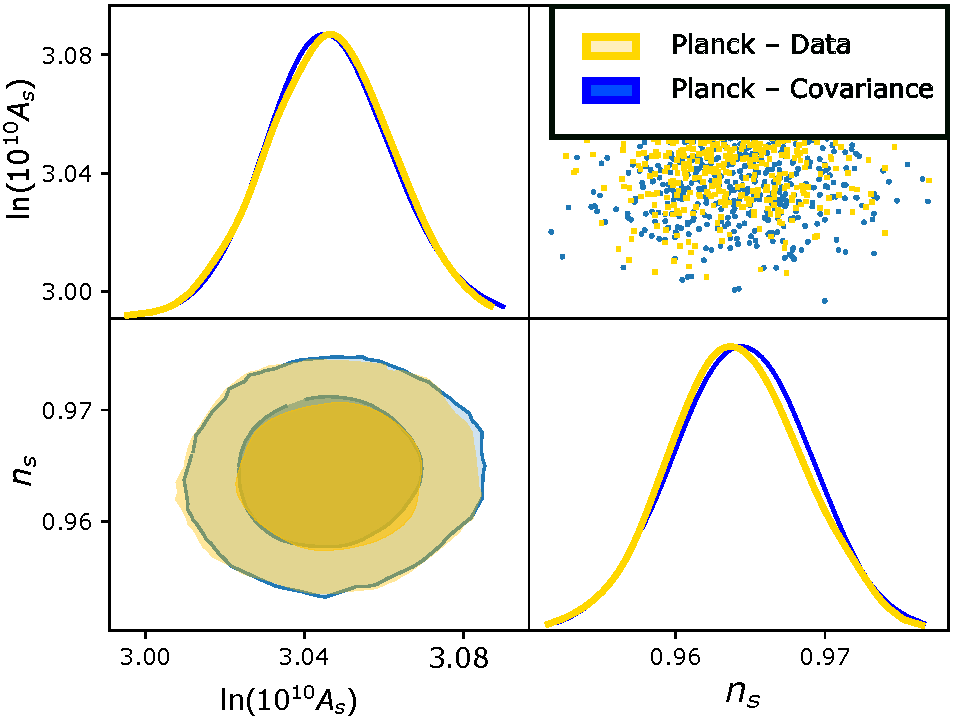
\includegraphics[width=0.5\textwidth]{./illustrations/triangle-fit.pdf}
\caption{An example of a posterior distribution generated with power posterior repartitioning, based on data from Planck. The posteriors are near identical, and a slight misfit can be explained with arithmetic rounding errors, and run-to-run variance of the position of the live points (see top right figure).\label{fig:overlay-posteriors}}
\end{figure}


\subsection{Simulations}
\subsubsection{Numerical models}

We shall begin our analysis with help of a simplified model that is
general-enough to share features with the Cosmological scale problem,
but also practical to investigate in depth, with multiple variations.

Our original model is a Gaussian peak. By choosing the uniform prior
as a baseline, and setting the log-likelihood as:
\begin{equation*}
  \ln {\cal L}(\bm{\theta}) = - \dfrac{1}{2} \left\{{(\bm{\theta} - \bm{\mu})}^{T}G^{-1}(\bm{\theta}-\bm{\mu})  + \ln \det \left| 2\mathrm{\pi} \bm{\Sigma}\right| \right\},
\end{equation*}
where the covariance matrix \(\bm{\Sigma}\), specifies the extent of
the peak, and the vector \(\bm{\mu}\), its location. We thus expect
the posterior to be a truncated and re-scaled Gaussian. However its
typical set is still approximately at a distance of the square root of
the diagonal elements of the covariance matrix form the peak,
i.e.~\emph{one standard deviation}.

The covariance matrix is positive semi-definite and symmetric, hence
it can be diagonalised \citep{taboga2017lectures}. If the covariance
matrix is diagonal, the Gaussian distribution is called
uncorrelated. If all diagonal elements are equal, then the Gaussian is
spherical with characteristic diameter given by
\(2\bm{\sigma} = 2\sqrt{\bm{\Sigma}}\), where \(\bm{\Sigma} = \Sigma \mathds{1}\).


Under such circumstances it's a matter of integrating \cref{eq:def-z}
to obtain the evidence. Most generally
\begin{equation}\label{eq:evidence}
   {\cal Z} = \cfrac{{\left( \sqrt{ \det \left| 2\mathrm{\pi} \bm{\Sigma} \right|} \right)}^{n}}{\bm{b}-\bm{a}}, 
\end{equation}
where \(n\) is the number of parameters in the model.

To simulate imperfections we shall consider translational offsets
between the intuition prior and the likelihood\footnote{for PR the
  breadth of the distributions is irrelevant.}.


\section{Results and Discussion.}\label{sec:org50493c6}
The first test case is an uncorrelated spherical Gaussian posterior
in three dimensions \[\mathcal{P}(\bm{\theta}) = G(\bm{\theta}; \bm{\mu} =
  (1,2,3),\bm{\sigma} = \mathds{1}).\] The corresponding evidence
(\cref{eq:evidence}) is \(\mathcal{Z}\approx-62.3\). First we shall
assume that the mean and standard deviation of all the
repartitioning schemes is exactly the same as that of the
posterior.

All but one repartitioning scheme yielded the correct evidence. The
resize-able uniform prior model was constructed to systematically
overestimating the evidence (\cref{fig:hist}) which is due to
underestimating the normalisation factor for
\(\mathcal{L}\).


We shall now show that repartitioning is able to drastically reduce
the run-time compared to using a uniform prior. More specifically,
guessing a posterior distribution and using repartitioning, one may
reduce the initial compression stage to virtually none.

Having proven the correctness of the runs, let's turn to performance
and benchmarks. The central metric is the number of \({\cal L}\)
evaluations. \cref{fig:benchmark} shows that mixture
repartitioning, produces a significant speed-up compared to even
power-posterior repartitioning. Moreover, the slope of the curve of
the number of \({\cal L}\) evaluations is much steeper for the
slower repartitioning schemes, indicating that for large numbers of
live points, mixture repartitioning yields an even greater
speed-up.



\begin{figure}
  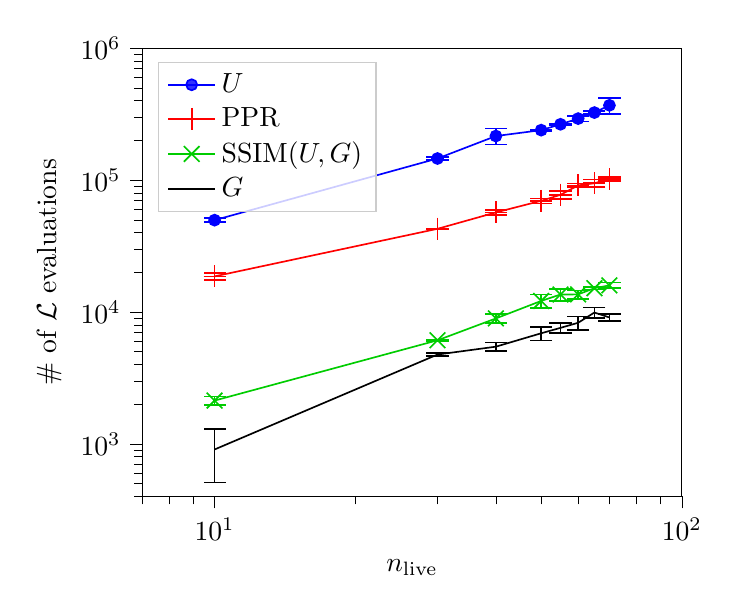
\begin{tikzpicture}

\definecolor{color0}{rgb}{0.0,0.0,1.0} %U
\definecolor{color1}{rgb}{1,0.0,0.0} %PPR
\definecolor{color2}{rgb}{0,0.8,0.0}                              %SSIM
\definecolor{color3}{rgb}{0.,0.0,0.0} %G

\begin{axis}[
legend cell align={left},
legend style={fill opacity=0.8, draw opacity=1, text opacity=1, at={(0.03,0.97)}, anchor=north west, draw=white!80!black},
tick align=outside,
tick pos=left,
x grid style={white!69.0196078431373!black},
xlabel={\(n_\text{live}\)},
xmin=7, xmax=100,
xtick style={color=black},
y grid style={white!69.0196078431373!black},
ylabel={\# of \({\cal L}\) evaluations},
ymin=400, ymax=1000000.0,
ytick style={color=black},
xmode=log,
ymode=log
]
\path [draw=color0, semithick]
(axis cs:10,48051.1762746562)
--(axis cs:10,51361.4903920105);

\path [draw=color0, semithick]
(axis cs:30,141787.579248368)
--(axis cs:30,149701.087418299);

\path [draw=color0, semithick]
(axis cs:40,185671.527674282)
--(axis cs:40,245784.472325718);

\path [draw=color0, semithick]
(axis cs:50,236296.832694899)
--(axis cs:50,241822.500638435);

\path [draw=color0, semithick]
(axis cs:55,262655.71356965)
--(axis cs:55,266952.953097016);

\path [draw=color0, semithick]
(axis cs:60,278243.015081106)
--(axis cs:60,306644.984918894);

\path [draw=color0, semithick]
(axis cs:65,317116.521541605)
--(axis cs:65,332736.145125062);

\path [draw=color0, semithick]
(axis cs:70,318358.948415036)
--(axis cs:70,419081.71825163);

\path [draw=color1, semithick]
(axis cs:10,17520.6487596482)
--(axis cs:10,19742.0179070185);

\path [draw=color1, semithick]
(axis cs:30,42472.9620658463)
--(axis cs:30,42994.371267487);

\path [draw=color1, semithick]
(axis cs:40,54281.6999405287)
--(axis cs:40,59494.3000594713);

\path [draw=color1, semithick]
(axis cs:50,66559.0160569084)
--(axis cs:50,72717.6506097582);

\path [draw=color1, semithick]
(axis cs:55,71552.6011973656)
--(axis cs:55,83118.7321359677);

\path [draw=color1, semithick]
(axis cs:60,88312.8386239607)
--(axis cs:60,94072.4947093726);

\path [draw=color1, semithick]
(axis cs:65,88215.9096228476)
--(axis cs:65,100992.090377152);

\path [draw=color1, semithick]
(axis cs:70,97882.04633)
--(axis cs:70,105637.95367);

\path [draw=color2, semithick]
(axis cs:10,1980.99743591911)
--(axis cs:10,2284.33589741422);

\path [draw=color2, semithick]
(axis cs:30,6035.87692136486)
--(axis cs:30,6174.12307863514);

\path [draw=color2, semithick]
(axis cs:40,8260.41435100755)
--(axis cs:40,9624.91898232578);

\path [draw=color2, semithick]
(axis cs:50,10733.0849396109)
--(axis cs:50,13538.9150603891);

\path [draw=color2, semithick]
(axis cs:55,12122.9645002052)
--(axis cs:55,15015.0354997948);

\path [draw=color2, semithick]
(axis cs:60,12622.7721075812)
--(axis cs:60,14593.2278924188);

\path [draw=color2, semithick]
(axis cs:65,14804.9685728395)
--(axis cs:65,15505.0314271605);

\path [draw=color2, semithick]
(axis cs:70,15158.1193669152)
--(axis cs:70,16693.8806330848);

\path [draw=color3, semithick]
(axis cs:10,511.628293172651)
--(axis cs:10,1305.03837349402);

\path [draw=color3, semithick]
(axis cs:30,4625.34584399058)
--(axis cs:30,4900.65415600942);

\path [draw=color3, semithick]
(axis cs:40,5045.39013421616)
--(axis cs:40,5880.60986578384);

\path [draw=color3, semithick]
(axis cs:50,6085.69651897324)
--(axis cs:50,7719.6368143601);

\path [draw=color3, semithick]
(axis cs:55,6959.0338647499)
--(axis cs:55,8215.63280191676);

\path [draw=color3, semithick]
(axis cs:60,7317.2571539732)
--(axis cs:60,9267.40951269347);

\path [draw=color3, semithick]
(axis cs:65,8986.02980736454)
--(axis cs:65,10838.6368593021);

\path [draw=color3, semithick]
(axis cs:70,8588.48027282128)
--(axis cs:70,9612.18639384539);


\addplot [semithick, color1, mark=-, mark size=4, mark options={solid}, only marks, forget plot]
table {%
10 17520.6487596482
30 42472.9620658463
40 54281.6999405287
50 66559.0160569084
55 71552.6011973656
60 88312.8386239607
65 88215.9096228476
70 97882.04633
};
\addplot [semithick, color1, mark=-, mark size=4, mark options={solid}, only marks, forget plot]
table {%
10 19742.0179070185
30 42994.371267487
40 59494.3000594713
50 72717.6506097582
55 83118.7321359677
60 94072.4947093726
65 100992.090377152
70 105637.95367
};
\addplot [semithick, color2, mark=-, mark size=4, mark options={solid}, only marks, forget plot]
table {%
10 1980.99743591911
30 6035.87692136486
40 8260.41435100755
50 10733.0849396109
55 12122.9645002052
60 12622.7721075812
65 14804.9685728395
70 15158.1193669152
};
\addplot [semithick, color2, mark=-, mark size=4, mark options={solid}, only marks, forget plot]
table {%
10 2284.33589741422
30 6174.12307863514
40 9624.91898232578
50 13538.9150603891
55 15015.0354997948
60 14593.2278924188
65 15505.0314271605
70 16693.8806330848
};
\addplot [semithick, color3, mark=-, mark size=4, mark options={solid}, only marks, forget plot]
table {%
10 511.628293172651
30 4625.34584399058
40 5045.39013421616
50 6085.69651897324
55 6959.0338647499
60 7317.2571539732
65 8986.02980736454
70 8588.48027282128
};
\addplot [semithick, color3, mark=-, mark size=4, mark options={solid}, only marks, forget plot]
table {%
10 1305.03837349402
30 4900.65415600942
40 5880.60986578384
50 7719.6368143601
55 8215.63280191676
60 9267.40951269347
65 10838.6368593021
70 9612.18639384539
};
\addplot [semithick, color0, mark=-, mark size=4, mark options={solid}, only marks, forget plot]
table {%
10 48051.1762746562
30 141787.579248368
40 185671.527674282
50 236296.832694899
55 262655.71356965
60 278243.015081106
65 317116.521541605
70 318358.948415036
};
\addplot [semithick, color0, mark=-, mark size=4, mark options={solid}, only marks, forget plot]
table {%
10 51361.4903920105
30 149701.087418299
40 245784.472325718
50 241822.500638435
55 266952.953097016
60 306644.984918894
65 332736.145125062
70 419081.71825163
};
\addplot [semithick, color0, mark=*, mark size=2, mark options={solid}]
table {%
10 49706.3333333333
30 145744.333333333
40 215728
50 239059.666666667
55 264804.333333333
60 292444
65 324926.333333333
70 368720.333333333
};
\addlegendentry{$U$}
\addplot [semithick, color1, mark=+, mark size=4, mark options={solid}]
table {%
10 18631.3333333333
30 42733.6666666667
40 56888
50 69638.3333333333
55 77335.6666666667
60 91192.6666666667
65 94604
70 101760
};
\addlegendentry{PPR}
\addplot [semithick, color2, mark=x, mark size=4, mark options={solid}]
table {%
10 2132.66666666667
30 6105
40 8942.66666666667
50 12136
55 13569
60 13608
65 15155
70 15926
};
\addlegendentry{$\text{SSIM}(U,G)$}
\addplot [semithick, color3, mark=., mark size=2, mark options={solid}]
table {%
10 908.333333333333
30 4763
40 5463
50 6902.66666666667
55 7587.33333333333
60 8292.33333333333
65 9912.33333333333
70 9100.33333333333
};
\addlegendentry{$G$}
\end{axis}

\end{tikzpicture}

\caption{comparison of likelihood calls necessary for obtaining the correct evidence for the case of a spherical uncorrelated Gaussian posterior. Note that almost all series scale linearly with the number of live points. \label{fig:benchmark}}
\end{figure}




The next trial involved a variable offset, where convergence to the
correct posterior and evidence is not guaranteed even with the correct
normalisation. For this case, we have taken the same Gaussian
truncated to a cube \(1000\times1000\times1000\). Two types of
sampling runs were considered: one where the posterior and prior
distributions coincided, and one with the mean of the posterior
shifted relative to the prior by an amount proportional to the mean
$\mu = (1,2,3)$.

The exemplary results are given in \cref{fig:convergence}.

The main notable feature is the inaccuracy of the posterior for
PPR. If the offset is small --- \(O(2\sigma)\), the posterior is
shifted. With a larger offset, e.g. \(O(4\sigma)\), two peaks can be
resolved, sadly, with less density near the correct Gaussian
peak. Both errors are compounded by incorrect evidence (see
\cref{fig:drift}) PPR: \(\ln {\cal Z}\approx -25.4 \pm 0.2\), vs
uniform reference \(\ln {\cal Z} = -22.7 \pm 0.4\).

In practice one has the following options:
\begin{enumerate}
\item accept the posterior as is~\label[Option]{opt:accept}
\item accept the posterior, but as a less credible result\label[Option]{opt:accept-with-err}
\item reject the PPR result entirely, and perform a run with only a
uniform prior\label[Option]{opt:uniform}
\item readjust the PPR mean and variance using the posterior, and
re-run~\label[Option]{opt:shift}
\item combine PPR with SSPR in mixture with a uniform prior
\end{enumerate}
\vref{opt:accept} is adequate for low accuracy standards provided the
error is properly estimated using a tool such as \texttt{nestcheck}.
From \cref{fig:benchmark}, we see that the performance uplift allows
for \cref{opt:shift} to be more efficient than~\ref{opt:uniform},
albeit marginally so. \Cref{opt:accept-with-err} is a last resort.

This is where our technique is most useful: one obtains, as we've
shown in~\cref{fig:convergence}, a more accurate
\({\cal P}(\bm{\theta})\), by using PPR from within SSPR. The
performance impact has considerable run-to-run variance, however never
exceeds \(20\%\) extra \({\cal L}\) evaluations, which is an order of
magnitude less than~\vref{opt:uniform,opt:shift} would afford.

\begin{figure}
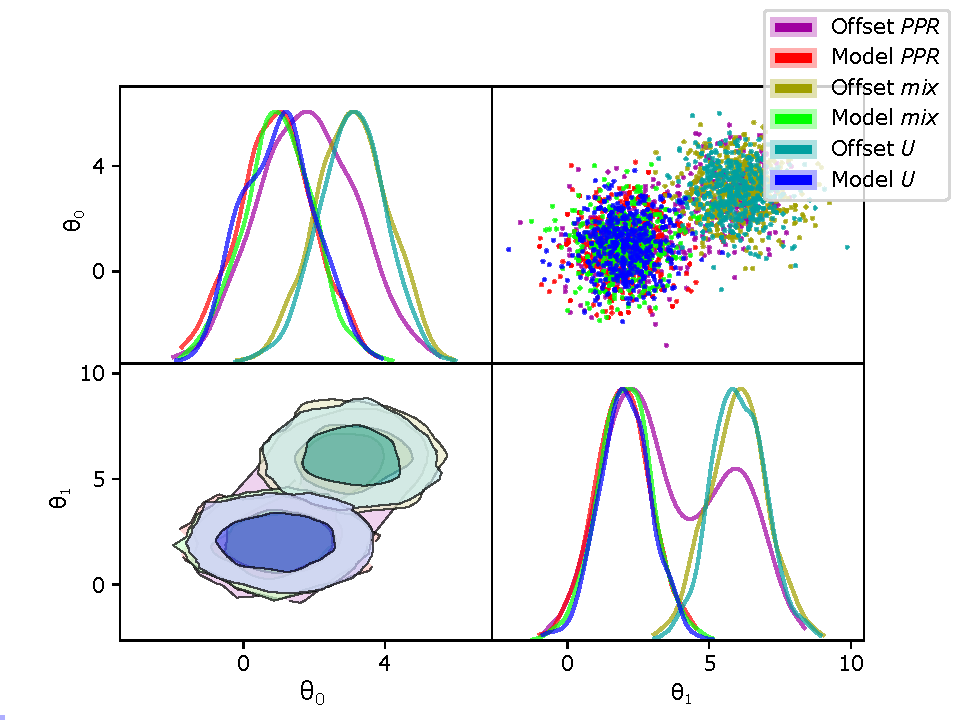
\includegraphics[width=0.5\textwidth]{./illustrations/convergence.pdf}
\caption{An illustration of how offsets affect the convergence of nested sampling under different kinds of repartitioning. The offset models should produce an offset posterior, whilst sharing the prior with the model runs. The mixture is of the present uniform model and PPR.\label{fig:convergence}}
\end{figure}

\begin{figure}
  % This file was created by tikzplotlib v0.9.1.
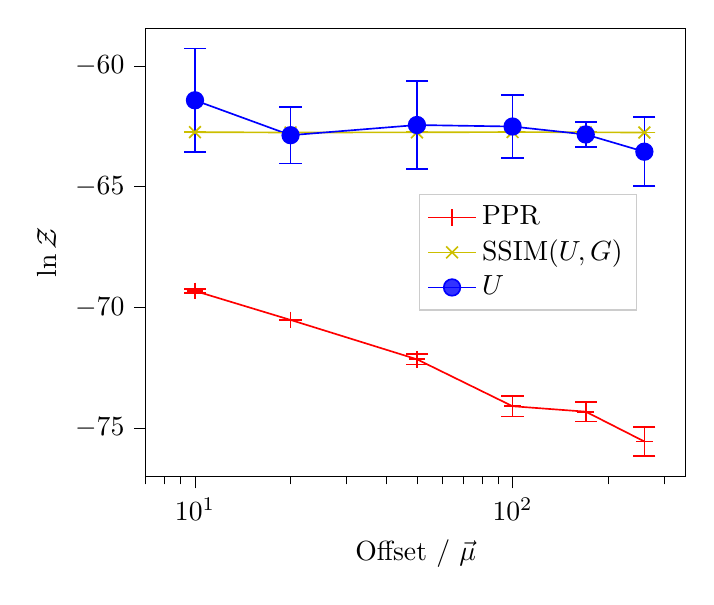
\begin{tikzpicture}

\definecolor{color0}{rgb}{1,0.0,0.0}
\definecolor{color1}{rgb}{0.8,0.75,0.0}
\definecolor{color2}{rgb}{0.0,0.0,1}

\begin{axis}[
legend cell align={left},
legend style={fill opacity=0.8, draw opacity=1, text opacity=1, at={(0.91,0.5)}, anchor=east, draw=white!80!black},
tick align=outside,
tick pos=left,
x grid style={white!69.0196078431373!black},
xlabel={Offset / \(\displaystyle \vec{\mu}\)},
xmin=-2.5, xmax=350.5,
xtick style={color=black},
y grid style={white!69.0196078431373!black},
ylabel={\(\displaystyle \ln {\cal Z}\)},
ymin=-77.013439988999, ymax=-58.4325947574349,
ytick style={color=black},
xmode=log
]
\path [draw=color0, semithick]
(axis cs:10,-69.4059960469118)
--(axis cs:10,-69.2379297037398);

\path [draw=color0, semithick]
(axis cs:20,-70.5299156173721)
--(axis cs:20,-70.5157474991409);

\path [draw=color0, semithick]
(axis cs:50,-72.3755951664078)
--(axis cs:50,-71.9328145858461);

\path [draw=color0, semithick]
(axis cs:100,-74.5305277482911)
--(axis cs:100,-73.6673769114354);

\path [draw=color0, semithick]
(axis cs:170,-74.7380053024013)
--(axis cs:170,-73.9121550603194);

\path [draw=color0, semithick]
(axis cs:260,-76.168856114837)
--(axis cs:260,-74.9518470928008);

\path [draw=color1, semithick]
(axis cs:10,-62.7439928102151)
--(axis cs:10,-62.7359696372663);

\path [draw=color1, semithick]
(axis cs:20,-62.755485458383)
--(axis cs:20,-62.7535773275597);

\path [draw=color1, semithick]
(axis cs:50,-62.7484141957878)
--(axis cs:50,-62.7468638775576);

\path [draw=color1, semithick]
(axis cs:100,-62.7369486572665)
--(axis cs:100,-62.7333125352419);

\path [draw=color1, semithick]
(axis cs:170,-62.746863877575)
--(axis cs:170,-62.745391448683);

\path [draw=color1, semithick]
(axis cs:260,-62.7574960930232)
--(axis cs:260,-62.7517661617973);

\path [draw=color2, semithick]
(axis cs:10,-63.5623386499016)
--(axis cs:10,-59.2771786315969);

\path [draw=color2, semithick]
(axis cs:20,-64.0348662974579)
--(axis cs:20,-61.6973543628668);

\path [draw=color2, semithick]
(axis cs:50,-64.2749108611421)
--(axis cs:50,-60.6135450768888);

\path [draw=color2, semithick]
(axis cs:100,-63.8144479355573)
--(axis cs:100,-61.1997313352197);

\path [draw=color2, semithick]
(axis cs:170,-63.3536082125541)
--(axis cs:170,-62.3180044247467);

\path [draw=color2, semithick]
(axis cs:260,-64.9781441262723)
--(axis cs:260,-62.1236339929356);

\addplot [semithick, color0, mark=-, mark size=4, mark options={solid}, only marks, forget plot]
table {%
10 -69.4059960469118
20 -70.5299156173721
50 -72.3755951664078
100 -74.5305277482911
170 -74.7380053024013
260 -76.168856114837
};
\addplot [semithick, color0, mark=-, mark size=4, mark options={solid}, only marks, forget plot]
table {%
10 -69.2379297037398
20 -70.5157474991409
50 -71.9328145858461
100 -73.6673769114354
170 -73.9121550603194
260 -74.9518470928008
};
\addplot [semithick, color1, mark=-, mark size=4, mark options={solid}, only marks, forget plot]
table {%
10 -62.7439928102151
20 -62.755485458383
50 -62.7484141957878
100 -62.7369486572665
170 -62.746863877575
260 -62.7574960930232
};
\addplot [semithick, color1, mark=-, mark size=4, mark options={solid}, only marks, forget plot]
table {%
10 -62.7359696372663
20 -62.7535773275597
50 -62.7468638775576
100 -62.7333125352419
170 -62.745391448683
260 -62.7517661617973
};
\addplot [semithick, color2, mark=-, mark size=4, mark options={solid}, only marks, forget plot]
table {%
10 -63.5623386499016
20 -64.0348662974579
50 -64.2749108611421
100 -63.8144479355573
170 -63.3536082125541
260 -64.9781441262723
};
\addplot [semithick, color2, mark=-, mark size=4, mark options={solid}, only marks, forget plot]
table {%
10 -59.2771786315969
20 -61.6973543628668
50 -60.6135450768888
100 -61.1997313352197
170 -62.3180044247467
260 -62.1236339929356
};
\addplot [semithick, color0, mark=+, mark size=3, mark options={solid}]
table {%
10 -69.3219628753258
20 -70.5228315582565
50 -72.154204876127
100 -74.0989523298633
170 -74.3250801813604
260 -75.5603516038189
};
\addlegendentry{PPR}
\addplot [semithick, color1, mark=x, mark size=3, mark options={solid}]
table {%
10 -62.7399812237407
20 -62.7545313929713
50 -62.7476390366727
100 -62.7351305962542
170 -62.746127663129
260 -62.7546311274102
};
\addlegendentry{SSIM$(U, G)$}
\addplot [semithick, color2, mark=*, mark size=3, mark options={solid}]
table {%
10 -61.4197586407493
20 -62.8661103301623
50 -62.4442279690155
100 -62.5070896353885
170 -62.8358063186504
260 -63.5508890596039
};
\addlegendentry{$U$}
\end{axis}

\end{tikzpicture}

\caption{Comparison of evidence estimates produced by different repartitioning schemes. The true value is constant, and should not depend on the offset. Mixture repartitioning is able to correctly cope with the offset, producing the correct evidence and posterior, while PPR is gradually drifting.\label{fig:drift}}
\end{figure}


Lastly, \emph{posterior mass} is a measure of converge
speed~\cite{higson2018nestcheck}, which is used in diagnosing
pathological issues specific to nested sampling. Typical examples for
uniform and re-partitioned priors are given in
plot~\Cref{fig:higson}. Firstly, note faster compression with
repartitioning, consistent with run-time reduction. Secondly, notice
that the re-partitioned series has a longer extinction phase, as a
result of introducing extra nuisance parameters. Finally, notice that
the confidence intervals for the parameters' distributions are near
identical, signifying that the obtained posteriors are more precise,
agreement with the constructed posterior:
\(G(\bm{\theta} = (0, 4, 8), \bm{\sigma} = 1)\), --- accurate.

\begin{figure}
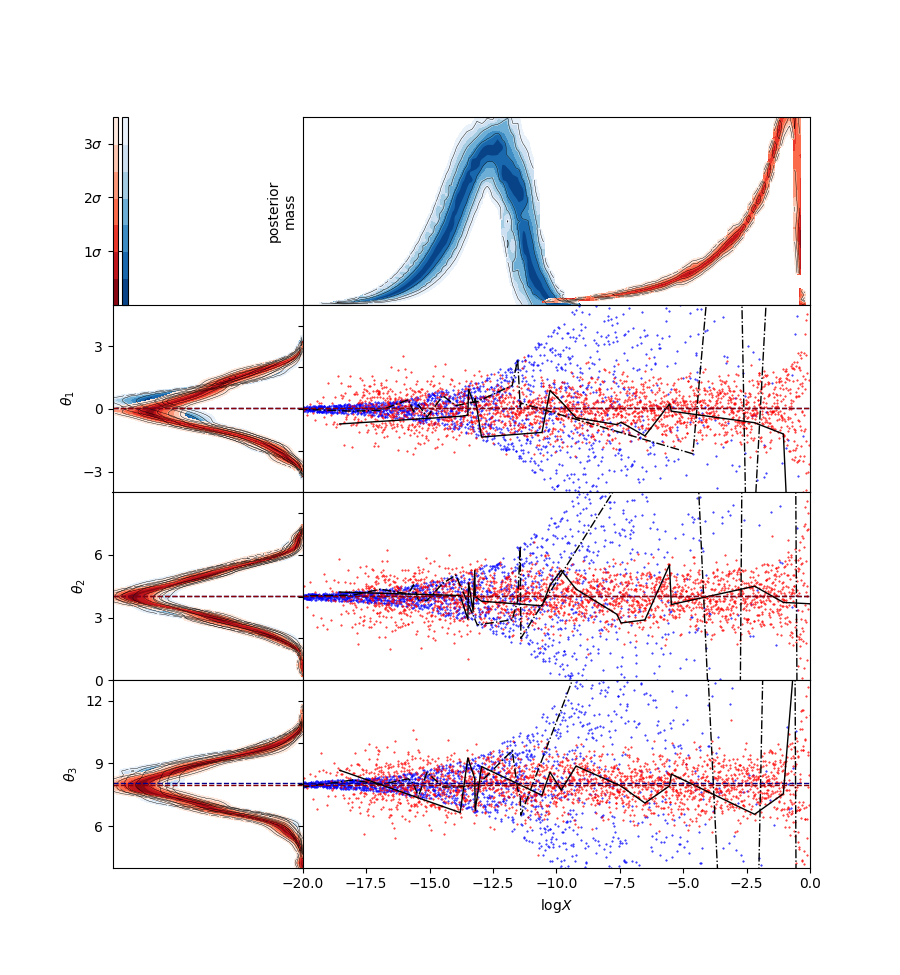
\includegraphics[width=.5\textwidth]{./illustrations/higson.png}
\caption{An evolutionary insight into the behaviour of nested sampling. The \color{red} red \color{black} series corresponds to mixture repartitioning, while the \color{blue} blue \color{black} series --- to a reference uniform. All plots are given in \(\ln X\), where \(X(\mathcal{L}) \in [0,1]\) is the fraction of the prior with likelihood greater than \(\mathcal{L}\). The top plot is the relative posterior mass, which is the total weight assigned to samples from the region. In each row, we're presented with the posterior in the given parameter. The gradients represent degree of confidence.\label{fig:higson}}
\end{figure}




\subsection{Cosmological Simulations.}\label{sec:orgb81c159}
After an initial run of \texttt{Cobaya}, we have obtained the marginalised
posteriors of all the key parameters of the \(\Lambda\)CDM model,
as well as the nuisance parameters.

Ignoring any off-diagonal elements of their co-variance, we have
constructed a mixture re-partitioned prior, containing a Gaussian
with our best estimates, a uniform containing the original
boundaries. A second run was thus performed.

Benchmarking on a cluster using time is impractical. Instead we
measured the number of likelihood calls for each invocation of
\texttt{PolyChord.run\_polychord()}.

The result is a \textbf{substantial} reduction in run-time.




\section{Conclusions}\label{sec:orgdf2cbd9}

\subsection{Results}\label{sec:orgc48c55d}
Our project's purpose had been to investigate the performance
increase attainable by algorithmic optimisations of the inputs to
nested samplers.

We have identified a general prescription, named superpositional
mixture repartitioning that netted the same if not greater
performance improvement as power posterior repartitioning (PPR).

We have also established that the aforementioned prescription had a
number of advantages:
\begin{enumerate}
\item it allows multiple priors to be mixed, while PPR only allows
one.
\item it permits a broader class of functions, than are practical for
PPR, e.g.~ones where \(Z_{\pi}(\beta)\) cannot be represented in
closed form.
\item it copes with functions having different domains. PPR cannot.
\item it is abstract, i.e.~the prior iCDF is a superposition iCDFs of
the constituents priors. For PPR the iCDF needs to be computed.
\item it supports an unbiased reference (uniform) prior exactly. PPR
tends to an unbiased reference as \(\beta\rightarrow\beta_{0}\).
\item it is able to mitigate improper re-scaling of the likelihood. If
one of the priors is improperly normalised, the offset from the
true evidence is reduced as \(n_{live}\rightarrow\infty\). PPR
does not.
\item it is resilient to human error.
\item it is easier to implement and requires little to no mathematical
input from the user, beyond ensuring the three properties.
\end{enumerate}


\subsection{Further research}\label{sec:org8314ddf}
The proposed algorithm of superpositional mixtures, maps neatly
onto concepts of quantum computation. Indeed one can model two
different priors as states of qubits. The benefits are potentially
immeasurable, as the greatest weakness of the classical algorithm
is that we're effectively sacrificing resolution in the posterior
by sampling only from one prior exclusively. Quantum superposition
allows us to do both at the same time, while quantum entanglement
ensures that the deterministic requirements set by
\citeauthor{Skilling2006} are met.

The necessary consequence of repartitioning is that the posterior
samples have a greater prior space to explore, and thus, while the
option to skip areas of negligible evidence allows us to compress
the priors significantly more quickly, the tail-end of the nested
sampling is also affected. A potential solution to this is to treat
the introduced parameters separately at this stage.

One such treatment may be to use the posterior distribution at the
point of discovery to freeze the choice parameters. Their
covariance may represent a volume in a \(\bm{\theta}\) space that
corresponds to the remaining evidence, and as such, crudely
approximate the remainder while sampling from a lower dimensional
space compounding to the physical (i.e.~not repartitioning-related
parameters of the theory).

Additionally, we have assumed that nested sampling converges the
fastest if the prior is also the posterior. However, a simple
example of a spherical Gaussian in three dimensions shows the same
characteristic tail at the end of the execution. It may be
necessary to look into priors that are tailor made to accelerate
that convergence. Naturally, they would also depend on the sampling
technique used: the prior that accelerates rejection sampling would
be different to one that accelerates slice sampling.

An additional avenue to explore would be to ask whether the same
sampling technique is appropriate for all stages. Slice sampling is
ideal for applications with prior space with large
dimensions. However, Metropolis-Hastings may be more suitable for
the extinction phase, and may thus eliminate the tail altogether.

Among the less-important investigations that could be carried out,
one might investigate an extension of the re-sizeable uniform
prior. Indeed one of the main reasons for its impracticality is the
sharp reduction to zero, that cannot be compensated for in the
likelihood. However, one should expect that this is possible to
compensate for by using a distribution that's constructed to be
non-zero in the entire domain of the original uniform prior:
e.g.~by having edges that tend to zero at the boundaries. A
suggestion might be a smooth top-hat, or a combination of error
functions.

\subsection{Applications}\label{sec:orgc67317e}
Nested sampling is a universal algorithm that can be applied to any
problem involving either direct parameter estimation (e.g.~analysis
of Planck data), or indirectly such as neural-network based machine
learning.

To clarify the latter point, the process of training a neural
network involves a process of estimating the connection strengths
between layers of states. Normally training is done via a negative
feedback process, where the connections that correspond to the
right answer are reinforced, whilst connections leading to
incorrect ones are reduced in strength. In the formalism of
Bayesian inference, the connection strengths are the parameters,
the prior is uniform and the sampling is done via
Metropolis-Hastings anticipating a logistical distribution. As we
are able to accelerate this process in Bayesian formalism, we
should also be able to modify the standard algorithms to make use
of repartitioning.

Moreover, the subject matter of this paper --- superpositional
mixture repartitioning with stochastic sampling may be used to
create classes of neural networks: as of now information obtained
from training one network cannot be re-used when training another,
unless the two networks have identical architecture and solve
identical problems. One cannot use the weights of a network
analysing faces as the initial values for analysing objects,
without that resulting in a strong bias.

It may be possible to use the values of node connection strengths
from networks that are used for similar problems, by virtue of the
stability offered by repartitioning. We can regard that as one of
the priors in the mixture, and hence improving performance where
the guess is indeed accurate, without compromising the result if it
is not. Of course such neural networks will need to have a similar
number of physical connections, and hence have similar if not
identical architecture.

\bibliography{bibliography}
\bibliographystyle{mnras}
\end{document}